%%
%% This code was generated from the thesis template of Adam Cooman--Evi Van Nechel.
%% It has been adapted slightly by Gustavo Quintana.
%% Compile with: 
%% cd C:\GusDocs\org\thesis\Gus-thesis
%% pdflatex --shell-escape -synctex=1 -interaction=nonstopmode Gus-thesis.tex 
%%
\documentclass[english, british, BCOR=5mm, DIV=12, fontsize=10pt]{scrbook}
\usepackage[T1]{fontenc}
\usepackage[latin9]{inputenc}
\usepackage[paperwidth=17cm, paperheight=24cm]{geometry} % \usepackage[hmargin=1.5cm, textheight=25cm]{geometry}
\geometry{verbose, tmargin=2.5cm, bmargin=3cm, lmargin=2.5cm, rmargin=2cm}
\setcounter{secnumdepth}{2}
\setcounter{tocdepth}{2}
\setlength{\parskip}{\medskipamount}
\setlength{\parindent}{0pt}
\synctex=-1
\usepackage{color}
\definecolor{note_fontcolor}{rgb}{0.800781, 0.800781, 0.800781}
\usepackage{amsfonts, amsmath, amssymb, amsthm, amsbsy, array, babel, booktabs, bm, float, graphicx, lineno, mathdots, mathptmx, mathtools, newproof, pgf, subcaption, textcomp, times, units, verbatim, xcolor}
\usepackage[unicode=true, pdfusetitle, bookmarks=true, bookmarksnumbered=false, bookmarksopen=false, breaklinks=true, pdfborder={0 0 0}, pdfborderstyle={}, backref=false, colorlinks=false]{hyperref}
\usepackage[outdir=./]{epstopdf}
\usepackage{tikz, circuitikz}
\usetikzlibrary{shapes, arrows, calc, patterns, decorations.pathmorphing, decorations.markings, positioning}

\newtheorem{thm}{Theorem}
\newtheorem{lem}[thm]{Lemma}
\newproof{pf}{Proof}

\DeclareMathAlphabet\mathbfcal{OMS}{cmsy}{b}{n}

\usepackage{algorithm, algorithmic}

\makeatletter

%%%%%%%%%%%%%%%%%%%%%%%%%%%%%% LyX specific LaTeX commands.
%% Because html converters don't know tabularnewline
\providecommand{\tabularnewline}{\\}
%% The greyedout annotation environment
\newenvironment{lyxgreyedout}
  {\textcolor{note_fontcolor}\bgroup\ignorespaces}
  {\ignorespacesafterend\egroup}

%%%%%%%%%%%%%%%%%%%%%%%%%%%%%% User specified LaTeX commands.
% font used for the math
\usepackage{mathptmx}
% font used for the text
\usepackage[nomath]{kpfonts}

% The microtype package improves the spacing between words and letters. 
\usepackage{microtype}

\usepackage[all]{nowidow}

% http://tex.stackexchange.com/questions/29973/more-than-one-optional-argument-for-newcommand
\usepackage{xparse}

% I remove some margin of the itemize list here I think.
\usepackage{enumitem}
% \setlist[itemize]{leftmargin=*}

% this will only add equation numbers to equations that have been referenced
% \usepackage{mathtools}
\usepackage{color,soul}

% this will make the bold omega available
\usepackage{bm}

% tables
\usepackage{tabularx}

% 
\usepackage{calc}
% tables 
\usepackage{multirow}

% figures and captions rotate 90 degrees
\usepackage{adjustbox}

% \thisfloatpagestyle{empty} for large figures/tables
\usepackage{floatpag}

% symbols for checkmarks
\usepackage{bbding}

% to include frontpage
\usepackage[final]{pdfpages}

% floats stay in section
\usepackage[section]{placeins}
%%%%%%%%%%%%%%%%%%%%%%%%%%%%%%%%%%%%%%%%%%%%%%%%%%%%%%%%%%%%%%%%%%%%
% For the Matlab2tikz plots, I include tikz
\usepackage{tikz}
\usepackage{pgfplots} 
\usepgfplotslibrary{groupplots}
\pgfplotsset{compat=newest} 
\pgfplotsset{plot coordinates/math parser=false} 
\usetikzlibrary{plotmarks}
\usepackage{grffile}
% stuff for the font size tiks pictures, you need to patch a bug in matlab2tikz for this to work though.
\pgfplotsset{every axis/.append style={font=\footnotesize}}
\pgfplotsset{tick label style={font=\footnotesize}}

% epsilon
\DeclareSymbolFont{newfont}{OML}{cmm}{m}{it}% Computer Modern math font
\DeclareMathSymbol{\Epsilon}{3}{newfont}{15}% Symbol 15


% figurelength and figureheight for tikz figures
\newlength\figureheight 
\newlength\figurewidth 
\setlength{\figurewidth}{0.8\columnwidth}
\setlength{\figureheight}{0.3\columnwidth}
\newlength\columnwidthex
\setlength{\columnwidthex}{0.9\columnwidth}

% \tikzify is used to create small tikz pictures in the lines of the text.
% I use this to put markers in my figure captions
% This code was provided to me by Jan Goos
\newcommand{\tikzify}[1]{\protect\tikz[baseline=-0.55ex]{\protect\draw[line width = 1pt] #1;}}
% \marker is used to add a specifiec marker in the text
\newcommand{\marker}[2]{\tikzify{plot[mark=#2,mark size=2.5,mark options={color=#1}](0,0)}}
\newcommand{\markerdot}[1]{\tikzify{plot[mark=*,mark size=1,mark options={color=#1}](0,0)}}

%%%%%%%%%%%%%%%%%%%%%%%%%%%%%%%%%%%%%%%%%%%%%%%%%%%%%%%%%%%%%%%%%%%%

% tables
\let\mytoprule\toprule
\renewcommand{\toprule}{\mytoprule[0.1 em]}
\let\mybottomrule\bottomrule
\renewcommand{\bottomrule}{\mybottomrule[0.1 em]}

%%%%%%%%%%%%%%%%%%%%%%%%%%%%%%%%%%%%%%%%%%%%%%%%%%%%%%%%%%%%%%%%%%%%
% page contains the specific changes made to the koma template

% set the page headers and footers in gray
\usepackage{scrlayer-scrpage}
\setkomafont{pageheadfoot}{\color{gray}\scslshape} %\textsl for italic

% chapter formatting
\addtokomafont{chapterprefix}{\raggedleft}
\renewcommand*{\chapterformat}{%
\mbox{\chapappifchapterprefix{\nobreakspace}%
Chapter \thechapter\autodot}\enskip}

% increase the line spacing
\linespread{1.1}

% set the footnotes in gray
\definecolor{footnotecolor}{cmyk}{0,0,0,0.75}
\setkomafont{footnote}{\color{footnotecolor}}

% set the footnote line in gray
\setkomafont{footnoterule}{\color{footnotecolor}}

% set the page number in gray
\addtokomafont{pagenumber}{\color{gray}\rmfamily}
\definecolor{pagenrcolor}{cmyk}{0,0,0,0}
\setkomafont{pagenumber}{\normalfont\bfseries\footnotesize\color{gray}}

% make all the titles bold
\setkomafont{disposition}{\normalfont\bfseries\fontfamily{pag}\selectfont}

\renewcommand*\chapterheadstartvskip{\vspace*{.15\textheight}}
\renewcommand*\chapterheadendvskip{\vspace*{.1\textheight}}
\renewcommand*{\chapterformat}{\chapappifchapterprefix{\ }\thechapter\autodot\enskip}

% define the VUB colors 
% I overwrite orange with the VUB orange and purple with the VUB blue
\definecolor{purple}{rgb}{0.007,0.25,0.51}
\definecolor{orange}{rgb}{1,0.35,0}

%%%%%%%%%%%%%%%%%%%%%%%%%%%%%%%%%%%%%%%%%%%%%%%%%%%%%%%%%%%%%%%%%%%%
% all abbreviations and symbols

\usepackage[toc,acronym,section=section,nonumberlist,xindy]{glossaries}
\renewcommand*{\acronymname}{List of Abbreviations}

\renewcommand{\newacronym}[4][]{\newglossaryentry{#2}{type=\acronymtype,
name={#3},
short={#3},
long={#4},
shortplural={#3\glspluralsuffix},
longplural={#4\glspluralsuffix},
description={#4},
text={#3},
first={#4~(#3)},
plural={#3\glspluralsuffix},
firstplural={#4\glspluralsuffix~(#3\glspluralsuffix)},
#1}}

\newacronym{BLA}{BLA}{Best Linear Approximation}
\newacronym{MIMO}{MIMO}{Multiple-Input Multiple-Output}
\newacronym{SISO}{SISO}{Single-Input Single-Output}
\newacronym{PISPO}{PISPO}{Periodic-In Same Period-Out}
\newacronym{FRF}{FRF}{Frequency Response Function}
\newacronym{ADS}{ADS}{Advanced Design System}
\newacronym{pdf}{pdf}{probability density function}
\newacronym{PSD}{PSD}{Power Spectral Density}
\newacronym{RMS}{RMS}{Root Mean Square}
\newacronym{LTI}{LTI}{Linear Time-Invariant}
\newacronym{RF}{RF}{Radio Frequency}
\newacronym{WLAN}{WLAN}{Wireless Local Area Network}
\newacronym{EM}{EM}{electromagnetic}
\newacronym{DGS}{DGS}{Defected Ground Structure}
\newacronym{RMSE}{RMSE}{Root Mean Square Error}
\newacronym{TL}{TL}{transmission line}
\newacronym{MC}{MC}{Monte Carlo}
\newacronym{SC}{SC}{Stochastic Collocation}
\newacronym{VF}{VF}{Vector Fitting}
\newacronym{LHS}{LHS}{Latin Hypercube Sampling}
\newacronym{QMC}{QMC}{Quasi Monte Carlo}
\newacronym{RBF}{RBF}{Radial Basis Functions}
\newacronym{PCBs}{PCBs}{Printed Circuit Boards}
\newacronym{PDNs}{PDNs}{Power Distribution Networks}
\newacronym{LDS}{LDS}{Low Discrepancy Sampling}
\newacronym{LBTLS}{LBTLS}{Local Bootstrapped Total Least Squares}
\newacronym{VNA}{VNA}{Vector Network Analyzer}
\newacronym{FOMs}{FOMs}{Figures of Merit}
\newacronym{FOM}{FOM}{Figure of Merit}
\newacronym{SNR}{SNR}{Signal-to-Noise Ratio}
\newacronym{SINAD}{SINAD}{Signal-to-Noise and Distortion ratio}
\newacronym{ACPR}{ACPR}{Adjacent Channel Power Ratio}
\newacronym{EVM}{EVM}{Error Vector Magnitude}
\newacronym{NPR}{NPR}{Noise Power Ratio}
\newacronym{DUT}{DUT}{Device Under Test}
\newacronym{TOI}{TOI}{Third Order Intercept point}
\newacronym{OFDM}{OFDM}{Orthogonal Frequency Division Multiplexing}
\newacronym{LTE}{LTE}{Long Term Evolution}



% \makeglossaries
\makenoidxglossaries







% to stop the compiler from complaining about the \it command in the references, I override it with the thing KOMA proposes.
\renewcommand{\it}{\normalfont\itshape}

% lyxgreyedout defined in latex
\renewenvironment{lyxgreyedout}
{\textcolor{red}\bgroup}{\egroup}

%\hyphenation{Lon-g-las-t-na-me}
\usepackage[square]{natbib}
\bibliographystyle{plainnat} % wmaainf  apalike

%%%%%%%%%%%%%%%%%%%%%%%%%%%%%% Start Document
\makeatother

\begin{document}
{\footnotesize{}}

%%%%%%%%%%%%%%%%%%%%%%%%%%%%%%  Front cover
%\includepdf[pages={1}]{Cover}
\newpage{}

%%%%%%%%%%%%%%%%%%%%%%%%%%%%%% VUB title page 

\titlepage{\fontfamily{pag}\selectfont % I use the ugly VUB font only for this title page
	\hspace{-0.1cm}
\includegraphics[width=0.4\columnwidth]{Extras/VUB_logo.pdf}
	% \vspace{-1.7cm}
	\hfill{}%
	\begin{minipage}[t]{0.4\columnwidth}% 
	\vspace{-1.4cm}
		\begin{flushright}
			{\footnotesize{}Department of }\\
			{\footnotesize{}Fundamental Electricity}\\
			{\footnotesize{}and Instrumentation (ELEC)}
		\par\end{flushright}%
	\end{minipage}


	\vspace{1.5cm}
	% I use purple and orange here for the color. In the preamble I have overwritten these colors to be VUB orange and VUB blue respectively
	\textcolor{purple}{\footnotesize{}Thesis submitted in fulfillment of the requirements for the degree of}\\
	\textcolor{purple}{\footnotesize{}Doctor of Engineering Sciences (Doctor in de Ingenieurswetenschappen) by}{\footnotesize\par}
	\textcolor{orange}{\Large{}ir. Gustavo Quintana Carapia}{\Large\par}

	\vspace{1cm}

	\begin{flushleft}
		\textcolor{purple}{\LARGE\noindent%\textcolor{purple}
		\textbf{Statistical analysis and experimental validation of data-driven dynamic measurement methods}}\\
	\par\end{flushleft}

	\vfill{}

	\begin{tabular}{@{}lll@{}}
	\textbf{\small PROMOTERS}		& &	{\small prof. dr. ir. Ivan Markovsky}				\\
				& &		{\footnotesize{}ELEC Department, Vrije Universiteit Brussel, Belgium}\\[0.3em]
				& &	\small prof. dr. ir. Rik Pintelon				\\
				& &		{\footnotesize{}ELEC Department, Vrije Universiteit Brussel, Belgium}	\\[0.3em]
				\\
	\textbf{\small MEMBERS OF THE JURY}	&	&\small prof. dr. ir. Patrick Guillaume (President)		\\
				&	&{\footnotesize{}MECH Department, Vrije Universiteit Brussel, Belgium}	\\[0.3em]
				% &								\\
				&	&\small prof. dr. ir. Roger Vounckx (Vice-President)				\\
				&	&{\footnotesize{}ETRO Department, Vrije Universiteit Brussel, Belgium}	\\[0.3em]
				% &								\\
				&	&\small dr. ir. Philippe Dreesen (Secretary)					\\
				&	&{\footnotesize{}ELEC Department, Vrije Universiteit Brussel, Belgium}				\\[0.3em]
				% &								\\
				&	&\small dr. ir. Nikolaos Deligiannis \\
				&	&{\footnotesize{}ETRO Department, Vrije Universiteit Brussel, Belgium} 			\\[0.3em]
				% &								\\
				&	&\small prof. dr. ir. Lyudmila Mihaylova 		\\
				&	&{\footnotesize{}ACSE Department, University of Sheffield, United Kingdom} \\
								% &								\\
				&	&\small prof. dr. ir. Stephane Chretien  		\\
				&	&{\footnotesize{}ERIC Laboratory, University Lyon 2, France} \\
								% &								\\
				&	&\small prof. dr. ir. Guillaume  Merc\`ere 		\\
				&	&{\footnotesize{}LIAS Laboratory, Universit\'e de Poitiers, France} \\
\end{tabular}

}

\newpage{}
%%%%%%%%%%%%%%%%%%%%%%%%%%%%%%  Book details

\pagenumbering{gobble}
~\vfill{}

% {\footnotesize{}ISBN: } \\% You need to apply online for an ISBN, this takes a couple of days
{\footnotesize{}DOI: 10.13140/RG.2.2.27482.29129}\\ % I uploaded my thesis to researchgate to generate a DOI: if you remove it from ResearchGate, the DOI will no longer exist!
{\footnotesize{}~}{\footnotesize\par}

{\footnotesize{}University Press BVBA}\\
{\footnotesize{}Rechtstro 2/001, 9185 Wachtebeke, Belgium }\\
{\footnotesize{}https://www.universitypress.be/}\\
{\footnotesize{}~}{\footnotesize\par}

{\footnotesize{}Vrije Universiteit Brussel, dept. ELEC}\\
{\footnotesize{}Pleinlaan 2, 1050 Brussel, Belgium}\\
{\footnotesize{}http://vubirelec.be/}\\
{\footnotesize{}~}{\footnotesize\par}

%{\footnotesize{}Cover design by ...}\\
%{\footnotesize{}Background image by ...}{\footnotesize\par}
%{\footnotesize{}~}{\footnotesize\par}

{\footnotesize{}$\copyright$ February 2020, Gustavo Quintana Carapia.}\\
{\footnotesize{}~}{\footnotesize\par}


{\footnotesize{}All rights reserved. No parts of this document may be reproduced or transmitted in any form or by any means without the prior written permission of the authors.}{\footnotesize\par}

{\footnotesize\par}

%%%%%%%%%%%%%%%%%%%%%%%%%%%%%%  Acknowledgements
\newpage{}
% \shipout\null
\pagenumbering{roman}

%% \documentclass{letter}
% \usepackage[T1]{fontenc}
% \usepackage[utf8]{inputenc}

% \begin{document}
\chapter*{Acknowledgements}
 I could not have done this without your support.

 \begin{quote}
\emph{Text.}\vfill{}
\end{quote}


Here comes your acknowledgement.
% \end{document}



%%%%%%%%%%%%%%%%%%%%%%%%%%%%%%  TOC and abbreviations list
\tableofcontents{}

% table of glossaries didn't work so I made a list of abbreviations manually
% I made my list of abbreviations manually because the glosseries didn't work
\chapter*{List of Abbreviations}
\begin{longtable}[c]{>{\raggedleft}p{0.2\columnwidth}>{\raggedright}p{0.7\columnwidth}}
\textbf{CRLB} &   Cram\'er-Rao Lower Bound\tabularnewline
\tabularnewline
\textbf{EIV} &  Errors in Variables\tabularnewline
\textbf{EWRLS} &  Exponentially Weighted Recursive Least Squares\tabularnewline
\tabularnewline
\textbf{FRF} &   Frequency Response Function\tabularnewline
\tabularnewline
\textbf{LS} &  Least Squares\tabularnewline
\textbf{LTI} &  Linear Time Invariant\tabularnewline
\textbf{LTV} &  Linear Time Varying\tabularnewline
\tabularnewline
\textbf{MC} &  Monte Carlo\tabularnewline
\textbf{ML} &  Maximum Likelihhod\tabularnewline
\textbf{MSE} &  Mean Squared Error\tabularnewline
\tabularnewline
\textbf{pdf} &  probability density function\tabularnewline
\textbf{PSD} &  Power Spectral Density\tabularnewline
\tabularnewline
\textbf{RLS} &  Recursive Least Squares\tabularnewline
\textbf{RMS} &  Root Mean Square \tabularnewline
\textbf{RMSE} &  Root Mean Square Error\tabularnewline
\tabularnewline
\textbf{SISO} &  Single-Input Single-Output\tabularnewline
\textbf{SNR} &   Signal-to-Noise Ratio\tabularnewline
\tabularnewline
\textbf{TV} &   Time Varying\tabularnewline

\end{longtable}
 

%%%%%%%%%%%%%%%%%%%%%%%%%%%%%%  Thesis
% CustomCommands.lyx contains my custom lyx math macros.
\selectlanguage{english}%
\global\long\def\norm#1{\left|#1\right|}%

\global\long\def\t{\!\left(t\right)}%

\global\long\def\jwk{\!\left(j\omega_{k}\right)}%

\global\long\def\k{\!\left(k\right)}%

\global\long\def\jw{\!\left(j\omega\right)}%

\global\long\def\BLA{^{\mathrm{BLA}}}%

\global\long\def\NL{\aleph}%

\global\long\def\GHz{\mathrm{\,GHz}}%

\global\long\def\MHz{\mathrm{\,MHz}}%

\global\long\def\um{\mathrm{\,\mu m}}%

\global\long\def\mm{\mathrm{\,mm}}%

\global\long\def\ohm{\mathrm{\,\varOmega}}%

\global\long\def\db{\mathrm{\,\mathrm{dB}}}%

\global\long\def\soo{S_{11}}%

\global\long\def\sot{S_{12}}%

\global\long\def\sto{S_{21}}%

\global\long\def\stt{S_{22}}%

\global\long\def\s{S_{11}\,\mathrm{and}\,S_{21}}%

\global\long\def\nF{\mathrm{\,nF}}%

\global\long\def\pF{\mathrm{\,pF}}%

\global\long\def\nH{\mathrm{\,nH}}%

\global\long\def\desiredE{-25\mathrm{\,dB}}%

\newcommand{\dgs}{\gls{DGS} }

%%% colors %%%
\definecolor{myBlue}{rgb}{0,0.4, 0.6}
\definecolor{MatlabBlue}{rgb}{0,0, 1}
\definecolor{myOrange}{rgb}{1,0.4,0}
\definecolor{myLightBlue}{rgb}{0.2980,0.7451,0.9333}
\definecolor{myYellow}{rgb}{1,0.7451,0.0549}
\definecolor{myGreen}{rgb}{0.4627,0.6706,0.1843}
\definecolor{green}{rgb}{0,0.5,0}
\definecolor{myGrey}{rgb}{0.55,0.55,0.55}
\definecolor{myBrown}{rgb}{0.6353,0.0784,0.1843}
\definecolor{myYellow}{rgb}{1,0.7451,0.0549}
\definecolor{myLightGrey}{rgb}{0.7,0.7,0.7}

%%% markers %%%

\newcommand{\blue}{\marker{myBlue}{-}\marker{myBlue}{-}}
\newcommand{\bluedash}{\marker{myBlue}{-} \marker{myBlue}{-}}
\newcommand{\orange}{\marker{myOrange}{-}\marker{myOrange}{-}}
\newcommand{\lbluedash}{\marker{myLightBlue}{-} \marker{myLightBlue}{-}}
\newcommand{\lblue}{\marker{myLightBlue}{-}\marker{myLightBlue}{-}}
\newcommand{\green}{\marker{myGreen}{-}\marker{myGreen}{-}}
\newcommand{\greendash}{\marker{myGreen}{-} \marker{myGreen}{-}}
\newcommand{\brown}{\marker{myBrown}{-}\marker{myBrown}{-}}
\newcommand{\browndash}{\marker{myBrown}{-} \marker{myBrown}{-}}
\newcommand{\yellow}{\marker{myYellow}{-}\marker{myYellow}{-}}
\newcommand{\yellowdash}{\marker{myYellow}{-} \marker{myYellow}{-}}
\newcommand{\lgreydash}{\marker{myLightGrey}{-} \marker{myLightGrey}{-}}
\newcommand{\matbluecirc}{\marker{MatlabBlue}{o}}
\newcommand{\orangecirc}{\marker{myOrange}{o}}
\newcommand{\orangex}{\marker{myOrange}{x}}
\newcommand{\bluecirc}{\marker{myBlue}{o}}
\newcommand{\bluetri}{\marker{myBlue}{triangle}}
\newcommand{\bluex}{\marker{myBlue}{x}}
\newcommand{\greencirc}{\marker{myGreen}{o}}
\newcommand{\greentri}{\marker{myGreen}{triangle}}
\newcommand{\greenx}{\marker{myGreen}{x}}
\newcommand{\yellowcirc}{\marker{myYellow}{o}}
\newcommand{\yellowdot}{\markerdot{myYellow}}
\newcommand{\bluedot}{\markerdot{myBlue}}
\newcommand{\lbluedot}{\markerdot{myLightBlue}}
\newcommand{\orangedot}{\markerdot{myOrange}}
\newcommand{\greendot}{\markerdot{myGreen}}

% \newcommand{\dash}{\marker{black}{$\dots$}}
\newcommand*\dash{\mathbin{\vcenter{\hbox{\rule{.4ex}{.4ex}}}\;\vcenter{\hbox{\rule{.4ex}{.4ex}}}\;\vcenter{\hbox{\rule{.4ex}{.4ex}}}}}

\selectlanguage{british}%



%!TEX root = ..\Thesis.tex
\chapter{Summary} \label{chap:Summary}
\vspace{-1.5cm}
Measurements are dynamical processes where the input is estimated using the sensor response. 
The users cannot wait for the sensor to reach a steady regime when the sensor response closely approximates the sensor static gain times the input. 
To obtain a fast input estimation, one approach is filtering the sensor transient response with another dynamical system, aiming to compensate the estimation time.
The compensator is commonly built after a sensor model to perform deconvolution.  
Another approach is estimating the input with data-driven methods that are independent from the sensor model.
Current digital signal processors (DSP) allow the implementation of both model-based and data-driven estimation methods.

There exists a data-driven method that directly estimates the step input level from the sensor step response. 
The formulation of this method is a Hankel-structure errors-in-variables (EIV) problem, where the regression matrix and the regressor are correlated.
The structured EIV problem is solved with recursive least-squares for real-time implementation.
The independence from the sensor model of the estimation method broadens its range of application.

The uncertainty of the step input estimation method is unknown and is not straightforwardly evident.
To validate the method for metrology applications, we studied the stochastic properties of the step input estimation.
A statistical analysis yields the estimation bias and variance, and thus, the estimation uncertainty.

Both with simulations and experiments, the sample mean squared error (MSE) of the step input estimation method is compared to its analytical Cram\'er-Rao bound.
The Cram\'er-Rao bound determines the minimum theoretical variance of the estimation.
It was found that the data-driven step input estimation is biased but has small variance, and the estimation MSE is less than one order of magnitude larger than the Cram\'er-Rao bound.
Moreover, in practical experiments, the step input estimation method is robust when the measurement noise is not Gaussian and white.

\begin{comment}
\section{Summary - Ramp input}

A measurement is a dynamical process that aims to estimate the true value of a measurand.
The measurand is the input that excites a sensor, and, as a consequence, the sensor output is a transient response. 
The main approach to estimate the input is applying the sensor transient response to another dynamical system. 
This dynamical system is designed by deconvolution to invert the sensor dynamics and compensate the sensor response. 
Digital signal processors enable an alternative approach to estimate the unknown input.
There exists a data-driven subspace-based signal processing method that estimates a measurand, assuming it is constant during the measurement.
To estimate the parameters of a measurand that varies at a constant rate, 
we extended the data-driven input estimation method to make it adaptive to the affine input.
In this paper, we describe the proposed subspace signal processing method for the measurement of an affine measurand and compare its performance to a maximum-likelihood input estimation method and to an existing time-varying compensation filter.
The subspace method is recursive and allows real-time implementations since it directly estimates the input without identifying a sensor model.
The maximum-likelihood method is model-based and requires very high computational effort.
In this form, the maximum-likelihood method cannot be implemented in real-time, however, we used it as a reference to evaluate the subspace method and the time-varying compensation filter results.
The effectiveness of the subspace method is validated in a simulation study with a time-varying sensor.
The results show that the subspace method estimation has relative errors that are one order of magnitude smaller and converges two times faster than the compensation filter.


\section{Summary - Statistical analysis}

A structured errors-in-variables (EIV) problem arising in metrology is studied.
The observations of a sensor response are subject to perturbation. 
The input estimation from the transient response leads to a structured EIV problem.
Total least squares (TLS) is a typical estimation method to solve EIV problems.
The TLS estimator of an EIV problem is consistent, and can be computed efficiently when the perturbations have zero mean, and are independently and identically distributed (i.i.d).
If the perturbation is additionally Gaussian, the TLS solution coincides with maximum-likelihood (ML).
However, the computational complexity of structured TLS and total ML prevents their real-time implementation.
The least-squares (LS) estimator offers a suboptimal but simple recursive solution to structured EIV problems with correlation, but the statistical properties of the LS estimator are unknown.
To know the LS estimate uncertainty in EIV problems, either structured or not, to provide confidence bounds for the estimation uncertainty, and to find the difference from the optimal solutions, the bias and variance of the LS estimates should be quantified.
Expressions to predict the bias and variance of LS estimators applied to unstructured and structured EIV problems are derived.
The predicted bias and variance quantify the statistical properties of the LS estimate and give an approximation of the uncertainty and the mean squared error for comparison to the Cram\'er-Rao lower bound of the structured EIV problem.

\section{Summary - Experimental validation}

Simultaneous fast and accurate measurement is still a challenging and active problem in metrology.
A sensor is a dynamic system that produces a transient response.
For fast measurements, the unknown input needs to be estimated using the sensor transient response.
When a model of the sensor exists, standard compensation filter methods can be used to estimate the input.
If a model is not available, either an adaptive filter is used or a sensor model is identified before the input estimation. 
Recently, a signal processing method was proposed to avoid the identification stage and estimate directly the value of a step input from the sensor response.
This data-driven step input estimation method requires only the order of the sensor dynamics and the sensor static gain.
To validate the data-driven step input estimation method, in this paper, the uncertainty of the input estimate is studied and illustrated on simulation and real-life weighing measurements.
It was found that the predicted mean-squared error of the input estimate is close to an approximate Cram\'er-Rao lower bound for biased estimators.
\end{comment}


%\newpage


\pagenumbering{arabic}

%!TEX root = ..\Thesis.tex
\chapter{Introduction} \label{chap:Introduction}

% Context:Metrology One of the objectives in metrology is the estimation of the true value of physical quantities.
Measurements are dynamical processes.
Sensors are dynamical systems that interact with physical quantities and deliver electrical signals.
This interaction is the input to the sensor and causes energy transferences that modify the sensor state.
The sensor response is the output that depends on both the input applied and the sensor initial conditions.

% Context:Tradeoff speed vs accuracy
There is a trade-off between speed and accuracy in a measurement.
The input excitation drives a linear time invariant sensor into a transient state, that is followed by a steady state.
During the sensor transient state, the response does not represent directly the input, but 
in steady state, the sensor response is proportional to the input.
The input can be estimated accurately from the sensor steady state response using the sensor static gain.
However, waiting for the steady state is not advisable for practical applications that need fast measurements.
In these applications the input must be estimated during the sensor transient state.

% Context:Compensation systems, # Context:Digital signal processing
One approach to estimate the input is filtering the sensor transient response with another dynamical system that inverts the dynamics of the sensor.
The filter output is an input estimate that compensates the measurement time.
The transient duration of the compensation filter is smaller than that of the sensor.
The compensator is designed to deconvolve the sensor response and is based on a sensor model.
Another approach is using digital signal processors (DSP).
DSPs are versatile since they allow the implementation of methods that do not necessarily recreate dynamic systems, such as digital filters.
A suitable model-independent, data-driven, method in a DSP can provide faster input estimations than with the model-based compensators.

% Context:Data-driven step input estimation method
An example of a data-driven method is the direct estimation of the step input level from the sensor step response \cite{Markovsky15cep}.
This method formulates a Hankel structured errors-in-variables (EIV) problem with correlation.
The regression matrix has a block-Hankel structure.
The regression matrix and the regressor are constructed from the transient response perturbed by measurement noise of zero mean and given variance.
The method is implemented in real-time using a recursive least-squares (RLS) solution of the structured EIV problem.
% Avoiding the model identification from input-output data and directly estimating the input from the transient response reduces the input estimation time and makes data-driven input estimation methods suitable for real-time 

% Context:Data-driven methodology
% The philosophy behind the estimation method is avoiding the explicit identification of a system model from input-output data and estimating directly the input from the transient response.
The main advantage of the data-driven input estimation method is that it does not identify the sensor model but instead it directly estimates the input. 
This differs from the classic two-stage methodology where the sensor model is first identified before the input is estimated.
In this method, the output-error (OE) problem is converted into an EIV problem that is harder to solve, but the RLS solution is easy to compute.
The range of application of the data-driven input estimation method is wide because it is independent of the sensor model.
The main disadvantage of the data-driven input estimation method is that its stochastic properties are not straightforwardly evident. 
It is more complex to find the stochastic properties of EIV problems when they have structure and correlation.
% Moreover, the online uncertainty assessment may not be feasible and we have to rely on confidence bounds.


% Problem under study: Dynamic measurements
% DM:Uncertainty assessment of data-driven input estimation methods
% DM:Experimental validation of the data-driven step input estimation method
The estimate uncertainty must be assessed to validate the estimation methods for metrology applications.
The uncertainty of the data-driven step input estimation method \cite{Markovsky15cep} is unknown.
The uncertainty can be defined in terms of the estimate bias and variance \cite{Pintelon12Book}, and these can be obtained by conducting an elementwise statistical analysis.
The validation of the step input estimation method requires also to demonstrate its effectiveness on real-life measurements.
In real-life experiments, the experimens were conducted with sensors of temperature and mass.
One challenge of using real-life data is that the noise may not fulfill the whiteness assumptions considered in the estimation problem formulation and in the statistical analysis.
The simulation and experimental results permit to compare the performance of the step input estimation method.

% DM:Estimation of affine input parameters
The ideas behind the step input estimation method raise the curiosity towards the design of estimation methods for other input models.
One of this input models is the ramp.
The ramp input estimation method is, in addition, motivated by the dynamic weighing that is performed in conveyor systems.
The dynamic weighing estimates the mass of materials or products during their transportation.
Ideally, when the conveyor belt transports the materials at a constant speed, i.e., the weighing sensor is excited with a ramp profile. 
The ramp is an affine input model that consists of two parameters, the slope and the interception.
The slope depends on the applied mass and can be used to estimate it from the transient response.
An adaptation of the step input estimation method can estimate the parameters of affine inputs.

\subsection{State of the art}
% StArt: Load cell sensors 
% experimental application is weighing
Weighing has been basic for the development of scientific and trade activites. 
The load cell is now a standard transducer for weight determination and also for the improvement of measurement techniques, such as the geometric approach to processing of load cell responses \cite{Kesilmis16}, the design of new conveyor machinery \cite{Yamani18}, and electronic truck scales \cite{Guo18}.

In safety studies, a six axis load cell is devised to quantify accelerations and impact forces exerted on a dummy \cite{Ballo16}.
In alternative energy developments the load cells are useful to measure the forces on the arms of a vertical axis wind turbine \cite{Rossander15}.
An academic study of the load that a structure withstands is conducted with strain gage load cells that confirms the numerical results and facilitates the design of complex shaped structures \cite{Olmi16}.
In sports, the performance of new instrumented crank mechanisms is fostered by the utilization of load cells in the characterization, analysis and validation design stages \cite{Casas16}.

The versatility of the load cells permits the physiological signal monitoring of the the heart and breathing rates \cite{Lee16}, clinical analysis of sleep quality \cite{Zahradka18} and the classification of the movement intensity of people while they are sleeping \cite{Alaziz17}. 
All of these experimental studies have load cells installed on bed setups.

% StArt:Compensation filters
The use of compensation filters for load cell sensor responses has been reported 
in \cite{Shu93}, where an adaptive digital filter was first explored,
in \cite{Jafaripanah05}, where an analog filter alternative was suggested,
in \cite{Hernandez06} where a recursive LS lattice adaptive filter improves tension forces measurement, 
in \cite{Boschetti13} where models of the weighing machine, load cells and accelerometers are exploited to remove the environmental vibrations effects, 
in \cite{Dienstfrey14} where the negative effects of the finite bandwidth of the measurement system response are diminished by regularized deconvolution, and
in \cite{Huang16}, where the noises that affect an electromagnetic-force-compensated load cell are removed with a set of filters.
Some guidelines to implement a compensation filter by deconvolution are described in \cite{Eichstadt10}, and
the synthesis of filters by mapping the sensor model parameters into the filter parameters and time reversed filtering is proposed in \cite{Hessling08a}.

% StArt:Digital signal processing estimation methods
% The use of a DSP in metrology motivated the data-driven step input estimation method \cite{Markovsky15cep}.
A short list of the DSP measurement methods for different physical quantities include 
the impact that the signal processing data-driven dynamic error correction has on the temperature uncertainty \cite{Saggin01},
the development of an electronic nose using bio-inspired signal processing techniques \cite{Jing16},
the impedance measurements for material damage estimation using cross-correlation signal processing techniques \cite{deCastro19},
the modulation quality measurement of microwave access systems is measured using digital signal processing \cite{Angrisani10}, and
the real-time rotational speed estimation using correlation signal processing techniques \cite{Wang14}.

% StArt:Uncertainty assessment 
% Monte Carlo sampling
% Deterministic sampling
In metrology, the result of a measurement is a random variable.
The measurement is inherently perturbed by noise and, therefore, the input estimation is represented with the two first statistical moments \cite{Ferrero06}.
There is a guide to assess the uncertainty of the quantity estimation \cite{GUM08}, but there is still a need to study of the uncertainty of estimation methods and many approaches have been proposed \cite{Esward09, Hessling10}.
Some of the measurement uncertainty analysis are reviewed in \cite{daSilva12}.
The Monte Carlo method has been shown to be an effective uncertainty evaluation tool in \cite{Cox06},
and supports the usefulness of simulation for quantifying measurement uncertainties by software \cite{Esward16}.
Another example of the Monte Carlo method is the dynamic measurement uncertainty evaluation of clinical thermometers described in \cite{Ogorevc16}.

% 
It is recommended to consider the uncertainties of all the measurement chain components \cite{Diniz17}, and to avoid the direct uncertainty propagation from the calibration towards the to-be-measured quantity.  
Methods for evaluating the uncertainty associated with the output of compensation filters have been investigated, such as for
a discrete-time infinite-response filter in \cite{Link09},
a discrete-time finite-response filter in \cite{Elster07, Elster08}, and
the Kalman filter in \cite{Eichstadt16b}.
All these works propagate the uncertanity through the filter but it is also necessary to upward the propagation up to the sensor model to include all systematic error contributions \cite{Hessling11}.

%
An extension of the methodology proposed for the data-driven step input estimation was formulated to estimate the parameters of an affine input that changes at a constant rate,  by signal processing of the sensor transient response.
This type of ramp inputs is observed in the measurement of mass during the transportation of products on conveyor systems, ranging from few grams \cite{Burmen09} to almost hundreds of kilograms \cite{Tasaki07}.
The data-driven affine input estimation method is proposed as an alternative to existing compensation filters, such as 
the time-variant low-pass filters introduced in \cite{Piskorowski08, Pietrzak14}, and
the combination of filters in cascade proposed in \cite{Niedzwiecki16a}.

\subsection{Original contributions}
% OrigContrib:Affine input estimation
% OrigContrib:Statistical analysis of structured EIV problems
% OrigContrib:Experimental validation of the step input estimation method 
In this thesis are proposed two methods for estimating affine input parameters.
The first method is an adaptation of the data-driven input estimation method and the second is a maximum likelihood method based on local optimization.
The adaptation consists of the use of exponential weighing for the recursive least squares solution of the structured errors-in-variables problem.
The exponential weight gives preference to recent samples over the older samples.
This forgetting factor considers that the newer samples are more relevant for the parameters estimation.
The maximum-likelihood method method simulates the response of a sensor model to an affine input. 
The to-be-minimized cost function is the sum of the squared differences between the actual and the simulated sensor responses. 
The maximum-likelihood method needs more computational resources, and can simultaneously estimate parameters of the sensor model, but in it current formulation cannot run in real time.

In this document is presented a statistical analysis of the least squares solution of the structured errors-in-variables problem that the data-driven step input estimation method formulates.
The statistical analysis provides expressions that predict the bias and variance of the step input estimate for given sample size and measurement noise variance.
The second order Taylor series expansion of the LS solution obtain was derived to find expressions for the bias and variance of the estimate.
The Crámer-Rao lower bound of the structured EIV problem was obtained and it was compared to the empirical mean-squared error of the estimate.
It was observed that the input estimation is biased but with small variance, and the difference between the empirical MSE and the theoretical minimum and was determined quantitatively.


In this work a series of experiments was conducted to validate the step input estimation method in real-life applications.
The experiments were realizations of the step input excitation using temperature and mass sensors.
The weighing setup was constructed to ensure repeatability and reproducibility of the experimental realizations.
The step responses were stored in sets of 100 elements, and the empirical statistical moment of the input estimates were computed from the sample mean and variance of the estimations.
The step input estimation method showed robustness when the measurement noise is not Gaussian and white as it was assumed in the theoretical analyses.
The results of the estimation method with respect to different sensor model order were compared and we found that increasing the order does not necessarily benefits the input estimation uncertainty.


\subsection{Intro of Chapter ramp input}

Measurements estimate the unknown value of a physical quantity, namely the measurand.
The to-be-measured physical quantity is applied as an input signal to a sensor. 
The sensor is a dynamical system and its output changes as a consequence of the input excitation and the sensor initial conditions.
The goal of a measurement is to estimate accurately the measurand value using the sensor transient response.
The transient response of a stable sensor decays to a steady state response.
In steady state, the most accurate estimation of the input true value is simply found using the sensor static gain.
However, the steady state is reached in theory after an infinite period of time and in practice we require fast estimations.
The trade-off between accuracy and speed exists in all measurements.

The measurand can be assumed to be constant or variable during the measurement.
A dynamic measurement is present when the fluctuations of the measurand impact on the input estimation.
A typical example of a dynamic measurement problem is a low-bandwidth sensor excited with a fast changing input.
Some characteristics of the input, like the minimum or maximum or the effects of the environment on the measured quantity, occur in small periods of time.  
The detection of the input characteristics is needed in several scientific and industrial applications such as measurements of temperature \cite{Saggin01}, pressure \cite{Matthews14}, acceleration \cite{Link07}, force \cite{Vlajic16, Hessling08a} and mass \cite{Shu93, Boschetti13}.

The solution to dynamic measurement problems is non-trivial.
An approach is to add a dynamical system to compensate the sensor transient response, inverting the effects of the sensor dynamics.
The purpose of such a compensator is to reduce the transient time.
The sensor dynamics are considered in the design of finite and infinite impulse response compensation digital filters based on deconvolution \cite{Eichstadt10} or synthesized to correct dynamic errors \cite{Hessling08a}. 
The model-based deconvolution design of compensators implies that the measurand true value should be known a-priori for certain applications, such as mass determinations \cite{Boschetti13, Niedzwiecki16b}.
In the literature most of the measurements systems are assumed linear time-invariant, but the compensation digital filters can be linear \cite{Tasaki07},  nonlinear \cite{Shu93} or time-varying \cite{Pietrzak14}.

The digital signal processors enable a different approach where the input estimation can be obtained with algorithms that do not necessarily recreate the dynamics of a system.
One of the authors of this paper proposed a data-driven signal processing method that estimates the measurand true value using subspace techniques \cite{Markovsky15cep, Markovsky15ieee}.
The subspace estimation method bypasses the model identification step to estimate the unknown input directly from the response data.
This method was developed to estimate inputs modeled as step functions of unknown scaling level.
We extended the subspace input estimation method to estimate the parameters of inputs that vary at a constant rate.

The inputs that vary at a constant rate are found in applications where the measurand activates the sensor gradually. 
An example of this activation is the measurement of mass while the to-be-weighted object is transported by a conveyor belt, and the profile of the input is a saturated ramp.
Current solutions to the weighing in motion are low pass filters that estimate the mass using the saturated ramp \cite{Tasaki07, Pietrzak14}.
The signal processing affine input estimation methods are motivated by the need to obtain the mass of the object from the ramp before it reaches saturation.
The ramp is parameterized as a straight line model where the slope and the interception are the parameters of interest.

This paper describes a subspace method for the estimation of the affine input parameters.
This method is a recursive algorithm that can be implemented in real-time since it has low computational cost.
The subspace method is independent of the sensor model and, therefore, it is suitable for a variety of applications.
The dynamic weighing is one of the applications and was chosen as an implementation example.
The effectiveness of the method is evaluated in a simulation study.
The performance of the proposed method is compared to that of a maximum-likelihood (ML) estimation method based on local-optimization and a time-varying compensation filter.
%We found that the subspace method obtains the slope estimate from the sensor transient response using the same assumptions of the data-driven step input estimation method.

The ML method resembles the model predictive control approach in the sense that a cost function is minimized iteratively to optimize the parameters of a sensor model using the observed sensor response in a receding time horizon \cite{Mayne14}.
The difference is that the ML method aims to estimate the unknown value of the affine input parameters instead of identifying a model and controlling the dynamic system.
The ML method is more appropriate for off-line processing of the sensor transient response.
Nevertheless, the ML method can estimate the parameters of the affine input, the parameters of a sensor model, and the initial conditions of the sensor.

The uncertainty of the subspace method is assessed using a Taylor expansion of the estimate and Monte Carlo random sampling approach \cite{Quintana19}.
The Monte Carlo approach requires a large set of generated random samples, and for simple systems it is the recommended method.
There exists a deterministic sampling approach to study the uncertainty propagation of complex systems \cite{Hessling13a, Hessling13b}. 
Deterministic sampling aims to represent the minimal statistical information that is relevant to the uncertainty estimation in a finite set.
The uncertainty of the ML method is assessed using the derivatives of the residual error that constructs the to-be-minimized cost function.
The covariance of the optimization method estimate is found using the inverse of the Hessian matrix \cite{Pintelon12Book}.


\subsection{Intro of Chapter statistical analysis}

Errors-in-variables (EIV) are linear estimation problems in which the regression matrix and the regressor are perturbed \cite{VanHuffel91Book}, \cite{Markovsky07overview}.
In structured EIV problems, the regression matrix has a given structure that depends on the problem formulation.
Hankel, Toeplitz, or other application-specific matrices appear in problems of metrology \cite{Markovsky15cep}, system identification \cite{Soderstrom07}, image restoration \cite{Feiz17}, nuclear magnetic resonance spectroscopy \cite{Cai16}, direction-of-arrival estimation \cite{Pan18}, and time-of-arrival estimation \cite{Jia18}.

In metrology, the direct estimation of the input from the sensor transient response is formulated as a structured EIV problem.
The only observed signal is the sensor output.
To estimate a step input, the regression matrix, and the regressor are built from the step response observations \cite{Markovsky15cep}, and
the structure in the regression matrix is block-Hankel.
This data-driven estimation methodology reduces the estimation time of the classical two-stage approach where a sensor model is first identified, and later the input is estimated using the sensor model \cite{Azam15, Niedzwiecki16a}.
%The problem is EIV because the perturbation of the sensor response gets into the regression matrix.

Total least-squares (TLS) is the typical estimator for unstructured EIV problems and is consistent when the perturbations have zero mean, and the covariance is a given positive definite matrix.
When the perturbations are i.i.d. normally distributed, the solution of the TLS is equivalent to that of the maximum likelihood estimator (ML) \cite{Markovsky07overview}. 
For structured EIV problems, the TLS estimator does not give general results since each specific structure requires a particular treatment \cite{VanHuffel07TLSeditorial}, and the ML estimator leads to non-convex optimization problems where finding the global optimum is not guaranteed \cite{Rhode14recursive}.
Moreover, the computational complexity of TLS and ML inhibits real-time implementation to solve structured EIV problems. 

The least-squares (LS) estimator is a suboptimal but simple solution to structured EIV problems that admits a recursive form for easy real-time implementations.
Some of the reported works that propose LS estimators for structured EIV problems include 
the design of a fast algorithm for matrices with small displacement rank \cite{Mastronardi07fast},
the study of the estimator consistency \cite{Palanthandalam10parameter},
the determination of the bias, and the mean squared error of the parameter estimates in the identification of AR models \cite{Kiviet12high} \cite{Kiviet14improved}, and
a discussion of the causes of bias and inconsistency in homogeneous estimators \cite{Yeredor04homogeneous}.

 In measurement applications, it is highly relevant to assess the uncertainty of the input estimate.
The uncertainty of the reported LS estimators for structured EIV problems has not been addressed, and then, remains unknown.
The estimator uncertainty is expressed using the estimation bias and covariance \cite{Pintelon12Book}.
To know the LS estimator uncertainty, we quantified the bias and the covariance of the LS solution of EIV problems in the unstructured and structured cases. 
This extends the perturbation analysis of the LS estimator of unstructured and uncorrelated problems that was investigated in \cite{Stewart90SPT} and in \cite{Vaccaro94}.
This paper presents a study of the statistics of the LS estimate of unstructured and structured EIV problems. 
 We provide a discussion of the unstructured case as a reference, to get an insight of the impact that the structure of the regression matrix and the correlation between the regression matrix and the regressor perturbations have on the uncertainty of the LS estimate.
The structured case is motivated by the metrology estimation problem \cite{Markovsky15cep}, where the EIV problem has a Hankel structure, and the perturbations are correlated.
The study of the metrology input estimate illustrates a methodology to conduct statistical analysis for any structured EIV problem.
The mathematical expectation of the second-order Taylor series expansion of the LS estimate boils down to expressions that quantify the first and second-order moments of the LS estimate.
Via Monte Carlo simulations, we validated the accuracy of the bias, and the covariance approximations.
The derived approximations predict the LS estimate bias, and the covariance, for given sample size and perturbation level.
The predicted variance gives the uncertainty of the LS estimate.
We observed that, for the step input estimation problem, the mean squared error of the LS estimate is near to the minimum variance limit given by the Cram\'er-Rao lower bound of the structured EIV problem.
 By following this methodology, the bias and variance of the solutions of EIV problems with other structures is determined, and therefore, the uncertainty of the estimate.


\subsection{Intro of Chapter experimental validation}

 In this paper we consider that a measurement is a dynamic process, where an input excites a dynamic system, the sensor, and causes a dynamic transient response that also depends on the initial conditions of the sensor.
The to-be-measured quantity is an unknown input that excites the sensor.
The consequent transient response is further processed to estimate quickly the measurand value.
The steady-state response of the sensor, that exists after the stabilization of dynamic effects, gives easy access to the measurand value but this approach is mainly exploited for calibration purposes.

A compensator is an additional dynamic system that acts on the transient response aiming to reduce the sensor transient time.
The compensation is motivated by the need of inverting the sensor dynamic effects to recreate the input.
The convolution of the compensator impulse response with the sensor transient response yields the input estimate.
Therefore, the design of a compensator is based on the sensor model and requires a deconvolution \cite{Eichstadt10}.
Examples of input estimation using compensation of the sensor transient response include a recursive estimation of the compensator parameters \cite{Shu93}, 
finite impulse response (FIR) \cite{Elster07, Niedzwiecki16b} filters and 
infinite impulse response (IIR) filters \cite{Pintelon90, Elster08}.
The filters in these works estimate in real-time the unknown input value.

An alternative to the compensation approach is to use digital signal processing methods that are independent of the sensor model.
A data-driven method that estimates the unknown level of step inputs by processing the sensor step response was introduced in \cite{Markovsky15ieee}. 
This data-driven input estimation method avoids the sensor modeling stage and estimates directly the input.
This method reduces the estimation time compared to a conventional compensator.
The step input estimation method performance was demonstrated by simulations and experiments on a digital signal processor (DSP) of low cost \cite{Markovsky15cep}.
The uncertainty of the step input estimation method has not been assessed before.

To validate the input estimation methods it is necessary to assess the uncertainty associated with their estimates \cite{daSilva12, Ferrero06}.
There are uncertainty propagation studies for model-based compensators such as the FIR and IIR filters for acceleration measurements where the uncertainty is computed in real time \cite{Elster07, Elster08, Link09}.
In these works, the uncertainty expression is based on the transfer function or state space representations of the LTI sensor and filter systems.
Another way to assess the measurement uncertainty is by observing the results of multiple practical measurements as it is described in \cite{Pietrzak14} for mass and in \cite{Ogorevc16} for temperature sensors.
A deconvolution method is implemented to estimate the input waveform in \cite{Hale09} and the uncertainty is obtained from the input estimate covariance. 
The impact that the signal processing data-driven dynamic error correction has on the uncertainty is investigated in \cite{Saggin01}. 
A statistical analysis of the data-driven step input estimation method \cite{Markovsky15cep} was investigated in \cite{Quintana19} and the method uncertainty was obtained with a Monte Carlo simulation study. 

This paper provides an uncertainty assessment of the data-driven step input estimation method in a real-life application.
The measurements were conducted in a weighing system based on a load cell sensor.
We observed that even when the whiteness assumptions of the measurement noise are not fulfilled, the step input estimation method still is able to provide a good estimation. 
We found that the mean squared error of the input estimate is near the Cram\'er-Rao lower bound of the EIV problem.
A confidence interval is provided for the input estimate in terms of the number of samples required to satisfy the accuracy specifications of the user. 

The novelty of the paper is threefold.
First, using the results of \cite{Quintana19}, that describes a statistical analysis of structured errors in variables (EIV) problems, in this paper we describe the statistical properties of a the data-driven step input estimation method in both simulation and a real-life experiments.
Second, this manuscript also presents the Cram\'er-Rao lower bound for unbiased estimators of the structured and correlated EIV problem that the step input estimation method formulates.
Using this bound we have the minimum mean-squared error (MSE) for this estimation problem that we use compare with the MSE computed from the predictions obtained after the statistical analysis.
The third novelty in this manuscript is the model order selection for the step input estimation method where we use the MSE to select the order that provides the smaller MSE with the lowest computational complexity.


 
 
 
 
 
 
\newpage


%\part{Model driven filter design}\label{part:Filter}

%!TEX root = ..\Thesis.tex
\glsresetall

\chapter{Preliminaries} \label{chap:Preliminaries}

\vfill{}

\section{Preliminaries} 

In metrology, we use the concepts of linear systems theory to estimate the value of an unknown quantity.
A sensor is considered to be a causal linear time-invariant (LTI) system.
The unknown quantity is the input $\mathbf{u}$ of the sensor, and the consequences of this excitation are a change in the sensor state $\mathbf{x}$, from the initial conditions $\mathbf{x}_{\text{ini}}$, and a transient response in the sensor output $\mathbf{y}$, see Figure \ref{fig:sysLTI}.  
A measurement estimates the input value using the sensor response.

\begin{figure}[htb!]
\centering
\begin{tikzpicture}[every node/.style={draw,outer sep=0pt,thick}] 

 \node (NB1) [minimum width=1.5cm,minimum height=0.75cm,xshift=0.0cm, yshift=0.0cm] {Sensor};
 \draw [-latex,thick] (NB1.east) ++(0,0) -- +(1.0cm,0);
 \draw [-latex,thick] (NB1.north) ++(-0.5cm,0.5) -- +(0.0cm,-0.5);
 \node[draw=none,fill=none] [above=of NB1,xshift=0.0cm,yshift=-1.0cm] {$\mathbf{x}_{\text{ini}}$};
 \node[draw=none,fill=none] [right=of NB1,xshift=-0.5cm,yshift=0.25cm] {$\mathbf{y}$};
 \draw [-latex,thick] (NB1.west) +(-1.0,0) -- +(0.0cm,0);
 
 \node[draw=none,fill=none] [left=of NB1, xshift=0.750cm,yshift=0.25cm] {$\mathbf{u}$};
 
 \end{tikzpicture}
 \caption{Block diagram of an LTI sensor. The input $\mathbf{u}$ excites the sensor and generates the sensor response $\mathbf{y}$. To estimate the input value it is necessary to process the response.} \label{fig:sysLTI}
 \end{figure}

The discrete-time state-space representation of an LTI system is
\begin{equation} \begin{aligned} \mathbf{x}(k+1) &= \mathbf{A} \mathbf{x}(k) + \mathbf{B} \mathbf{u}(k), \quad \text{with} \quad \mathbf{x}_{\text{ini}} = \mathbf{x}(0) \\ 
\mathbf{y}(k) &= \mathbf{C} \mathbf{x}(k) + \mathbf{D} \mathbf{u}(k) + \mathbf{\nu}(k),  \label{eqn:dtsslti} \end{aligned} \end{equation}
where $\mathbf{A} \in \mathbb{R}^{n \times n}$, $\mathbf{B} \in \mathbb{R}^{n \times m}$, $\mathbf{C} \in \mathbb{R}^{p \times n}$, and $\mathbf{D} \in \mathbb{R}^{p \times m}$, are the model matrices, $\nu$ is the measurement noise, $n$ is the system order, $m$ is the number of inputs, and $p$ is the number of outputs.
Although we may think that most sensors are single-input single output (SISO) like temperature sensors, there are sensors with single input and multiple outputs such as gas sensors \citep{Munther19}, and sensors with multiple inputs and multiple outputs like the three-axis accelerometers \citep{DEmilia16}, the radio-frequency intruder-detection sensors \citep{Ushiki13}, and the radar sensor \citep{Kueppers17}.

The discrete-time state-space representation suggests that when the model, and the initial conditions are known, and in absence of measurement noise, it is sufficient to solve the system of equations 
\begin{equation} 
\underbrace{ \begin{bmatrix} y(0) \\ y(1) \\ y(2) \\ \vdots \\ y(T) \end{bmatrix} }_{\mathbf{y}}}
 = \underbrace{ \begin{bmatrix} \mathbf{C} \\ \mathbf{C} \mathbf{A} \\ \mathbf{C} \mathbf{A}^2 \\ \vdots \\ \mathbf{C} \mathbf{A}^T \end{bmatrix} }_{\mathbfcal{O}}} \mathbf{x}(0) +
 \underbrace{ \begin{bmatrix} \mathbf{D} \\ \mathbf{C} \mathbf{B} & \mathbf{D} \\ \mathbf{C} \mathbf{A} \mathbf{B} & \mathbf{C} \mathbf{B} & \mathbf{D} \\ \vdots & \ddots \\ \mathbf{C} \mathbf{A}^{T-1} \mathbf{B} & \cdots  &  \mathbf{C} \mathbf{A} \mathbf{B} & \mathbf{C} \mathbf{B} & \mathbf{D} \end{bmatrix} }_{\mathbfcal{T}}}
\underbrace{ \begin{bmatrix} u(0) \\ u(1) \\ u(2) \\ \vdots \\ u(T) \end{bmatrix} }_{\mathbf{u}}} ,
 \label{eqn:knownmodel} \end{equation}
to find the input. 
This system of equations is constructed from the recursions of (\ref{eqn:dtsslti}), where $\mathbfcal{O}$ is the observability matrix of the system, and $\mathbfcal{T}$ is a Toeplitz matrix of the Markov parameters of the system.
# formulated as the input estimation problem from the response of a system.

The input estimation problem is more complex when one or more of these assumptions are not fulfilled.
If the initial conditions and the measurement noise are unknown, the typical approach is to feed the output $\mathbf{y}$ to an additional system.
This additional system is modeled to invert the dynamics of the sensor by doing an operation that is equivalent to deconvolution, aiming to estimate the input $\mathbf{u}$ with the output $\widehat{\mathbf{u}}$ of the additional system.
This system is called compensator because the transient time of the estimated input $\widehat{\mathbf{u}}$ is smaller than the transient time of $\mathbf{y}$, see Figure \ref{fig:compensator}.  

\begin{figure}[htb!]
\centering
\begin{tikzpicture}[every node/.style={draw,outer sep=0pt,thick}] 

 \node (NB1) [minimum width=1.5cm,minimum height=0.75cm,xshift=0.0cm, yshift=0.0cm] {Sensor};
 \draw [-latex,thick] (NB1.east) ++(0,0) -- +(1.0cm,0);
 \draw [-latex,thick] (NB1.north) ++(-0.5cm,0.5) -- +(0.0cm,-0.5);
 \node[draw=none,fill=none] [above=of NB1,xshift=0.0cm,yshift=-1.0cm] {$\mathbf{x}_{\text{ini}}$};
 \node[draw=none,fill=none] [right=of NB1,xshift=-0.5cm,yshift=0.25cm] {$\mathbf{y}$};
 \draw [-latex,thick] (NB1.west) +(-1.0,0) -- +(0.0cm,0);
 
 \node[draw=none,fill=none] [left=of NB1, xshift=0.750cm,yshift=0.25cm] {$\mathbf{u}$};

\node (NB2) [minimum width=1.5cm, minimum height=0.75cm, xshift=2.9cm, yshift=0.0cm] {Compensator}; 
 \draw [-latex,thick] (NB2.north) ++(-0.5cm,0.5) -- +(0.0cm,-0.5);
 \node[draw=none,fill=none] [above=of NB2,xshift=0.0cm,yshift=-1.0cm] {$\mathbf{x}_{\text{ini,c}}$};
 \draw [-latex,thick] (NB2.east) ++(0,0) -- +(1.0cm,0);
 \node[draw=none,fill=none] [right=of NB2,xshift=-0.5cm,yshift=0.25cm] {$\widehat{\mathbf{u}}$};

 \end{tikzpicture}
 \caption{Input estimation using a compensator that processes the sensor response $\mathbf{y}$. The compensator is an additional system that reverts the dynamics of the sensor.} \label{fig:compensator}
 \end{figure}

If a model of the sensor is not available, the first idea may be to identify a model using the inputs and outputs, and later to estimate the input using the identified model.
However, the input is unknown and the model must be identified using only the sensor output.
Modeling the input as a multiple of the unit step function allows an analytical treatment of the input estimation problem.
This chapter describes step input estimation methods derived from linear systems theory. 
The description starts with the case in which the model is known, continues with the unknown sensor model case that performs model identification, and ends with a direct estimation of the input without model identification.
# The suitability of data-driven methods on-line implementation is higher because there is no need for high computational power to identify the system.


Step input estimation with system model

With a step input $\mathbf{u} = \bar{\mathbf{u}} s$, where $s(t) = 1$, for $t \geq 0$, and $s(t) = 0$, for $t < 0$, the discrete-time state space representation of the LTI sensor is equivalent to an augmented autonomous system  
\begin{equation} \begin{aligned} \mathbf{x}_\text{a}(k+1) &= \underbrace{ \begin{bmatrix} \mathbf{A} & \mathbf{B} \\ 0 & 1 \end{bmatrix} }_{\mathbf{A}_\text{a}} \mathbf{x}_\text{a}(k) , \quad \text{where} \ \ \mathbf{x}_\text{a}(k) = \begin{bmatrix} \mathbf{x}(k) \\ \mathbf{u}(k) \end{bmatrix}, \ \ \mathbf{x}_{\text{ini}} = \mathbf{x}(0) \\
\mathbf{y}(k) &= \underbrace{ \begin{bmatrix} \mathbf{C} & \mathbf{D} \end{bmatrix} }_{\mathbf{C}_\text{a}} \mathbf{x}_\text{a}(k) . \label{eqn:augmented} \end{aligned} \end{equation}
The eigenvalues $\lambda$ of the augmented autonomous system are found using
\[ \left| \lambda \mathbf{I} - \mathbf{A}_\text{a} \right| = \left| \lambda \mathbf{I} - \begin{bmatrix} \mathbf{A} & \mathbf{B} \\ 0 & 1 \end{bmatrix} \right| = \left| \lambda \mathbf{I} - \mathbf{A} \right| \left( \lambda - 1 \right) = 0.\]
Therefore, the eigenvalues, poles, of the augmented autonomous system (\ref{eqn:augmented}) are the eigenvalues, poles, of the LTI system, with the additional eigenvalue $\lambda = 1$, pole at $(1,0)$.  

Since the input $\mathbf{u}(t+1) = \mathbf{u}(t)$, for $t \geq 0$, is an augmented state of the autonomous system, and the system is known, a state estimator is sufficient to estimate the input.
In these conditions, the Kalman filter estimates recursively the input value.  

Step input estimation without system model

Reduction to autonomous equivalent model 

A first method, when the model of the LTI sensor is unknown and we have exact data, identifies a model of the sensor from the step response, and the estimates the input using the identified sensor model.
The model identification consists in the estimation of the matrices $\widehat{\mathbf{A}}_\text{a}$ and $\widehat{\mathbf{C}}_\text{a}$, and the initial conditions $\widehat{\mathbf{x}}(0)$.
To do this, consider that a Hankel matrix $\mathbfcal{H}(\mathbf{y}) \in \mathbb{R}^{n \times n}$, constructed from any linearly independent $n$ autonomous responses from the sensor initial conditions, is full column rank.
Thus, we can express 
\[ \underbrace{ \begin{bmatrix} y(1) & y(2) & \cdots & y(n) \\ y(2) & y(3) & \cdots & y(n+1) \\ \iddots & \iddots & \iddots \\ y(n) & y(n+1) & \cdots & y(2n-1) \end{bmatrix} }_{ \mathbfcal{H}(\mathbf{y}) }= \underbrace{ \begin{bmatrix} \widehat{\mathbf{C}}_\text{a} \\ \widehat{\mathbf{C}}_\text{a} \widehat{\mathbf{A}}_\text{a} \\ \vdots \\ \widehat{\mathbf{C}}_\text{a} \widehat{\mathbf{A}}_\text{a}^{n} \end{bmatrix} }_{ \mathbfcal{O}_\text{a} }  \underbrace{ \begin{bmatrix} \mathbf{x}_\text{a}(0) & \mathbf{x}_\text{a}(1) & \cdots & \mathbf{x}_\text{a}(n) \end{bmatrix} }_{ \mathbf{X}_\text{ini} } , \]
where $\mathbf{X}_\text{ini}$ is a matrix with the initial conditions of the $n$ free responses. 
A singular value decomposition of $\mathbfcal{H}(\mathbf{y})$ 
\[ \mathbf{U} \bm{\Sigma} \mathbf{V} = \mathbfcal{H}(\mathbf{y}), \]
permits the estimation of the observability matrix $\mathbfcal{O}_\text{a}$ and the initial conditions $\mathbf{X}_\text{ini}$, for example, by choosing
\[ \widehat{\mathbfcal{O}}_\text{a} = \mathbf{U} \sqrt{\bm{\Sigma}}, \quad \text{and} \quad \widehat{\mathbf{X}}_\text{ini} = \sqrt{\bm{\Sigma}} \mathbf{V} . \]
The matrices $\widehat{\mathbf{A}}_\text{a}$ and $\widehat{\mathbf{C}}_\text{a}$ can be estimated, from $\widehat{\mathbfcal{O}}_\text{a}$, by solving a system of equations.
In order to estimate the input, it is necessary to find a minimal representation of the autonomous system, by doing a linear transformation that removes the pole at $(1,0)$, and recovers the matrices $\widehat{\mathbf{A}}, \widehat{\mathbf{B}}, \widehat{\mathbf{C}}$, and $\widehat{\mathbf{D}}$.  

Identification of the model followed by input estimation

A second method is proposed to estimate the step input when the model of the LTI system is unknown but its steady-state gain $\mathbf{G}$ is known.   
Using the steady-state gain $\mathbf{G}$, we can express $\bar{\mathbf{y}} = \mathbf{G} \bar{\mathbf{u}}$, where $\bar{\mathbf{u}}$ is the input exact value and $\bar{\mathbf{y}}$ is the sensor steady state response.
The total response of the system is the sum of the transient and the steady-state responses.
Thus, considering the augmented autonomous model, we can write
\[ \mathbf{y} = \mathbf{G} \ \bar{\mathbf{u}} \ + \ \mathbfcal{O}_\text{a} \ \mathbf{x}(0) , \]
that in matrix form is
\[ \underbrace{ \begin{bmatrix}y(0) \\ y(1) \\ \vdots \\ y(T) \end{bmatrix}}_{\mathbf{y}} = \underbrace{ \begin{bmatrix} \mathbf{G} & \mathbf{C}_\text{a} \\ \mathbf{G} & \mathbf{C}_\text{a} \mathbf{A}_\text{a} \\ \vdots & \vdots \\ \mathbf{G} & \mathbf{C}_\text{a} \mathbf{A}_\text{a}^T \end{bmatrix}}_{\mathbf{K}} \begin{bmatrix} \bar{\mathbf{u}} \\ \mathbf{x}(0) \end{bmatrix} .\]
It is necessary to estimate the observability matrix of the augmented system, followed by the estimation of the input  $\mathbf{u}$, and the initial conditions $\mathbf{x}_{\text{ini}}$, using least squares
\[ \begin{bmatrix} \widehat{\mathbf{u}} \\ \widehat{\mathbf{x}}_{\text{ini}} \end{bmatrix} = \left( \mathbf{K}^\top \mathbf{K} \right)^{-1} \mathbf{K}^\top \mathbf{y}. \]

Data-driven estimation of an unknown step input given system response

A third method directly estimates the input value from the step response, without an identification of the sensor model.
Applying the first difference operator, $\Delta = \sigma - 1$, to the system state space representation (\ref{eqn:dtsslti}), we have
\begin{equation} \begin{aligned} \Delta \mathbf{x}(k+1) = \mathbf{A} \Delta \mathbf{x}(k), \quad \Delta \mathbf{y}(k) = \mathbf{C} \Delta \mathbf{x}(k), \quad \text{with} \quad \Delta \mathbf{x}_{\text{ini}} = \Delta \mathbf{x}(0) , \label{eqn:ssalti} \end{aligned} \end{equation}
where $\sigma$ is the shift operator, defined as $(\sigma^\tau y) (t) = y(t + \tau)$, and
$\Delta \mathbf{u}(k) = \mathbf{0}$, for $k \geq 0$, because we have a step input, and
$\Delta \mathbf{x}(0) = (\mathbf{A} - \mathbf{I}) \mathbf{x}(0) + \mathbf{B} \bar{\mathbf{u}}$.
The resulting system (\ref{eqn:ssalti}) is autonomous.
When the response $\Delta \mathbf{y}$ is persistingly exciting of order $L$, i.e., when the rank of the Hankel matrix $\mathbfcal{H}_{L+1}(\Delta \mathbf{y})$ of $L+1$ block rows constructed from $\Delta \mathbf{y}$ satisfies
\[\mathrm{rank} \left( \mathbfcal{H}_{L+1} \left( \Delta \mathbf{y} \right) \right) \leq L,  \]
the Hankel matrix $\mathbfcal{H}_{L+1}(\Delta \mathbf{y})$ provides a linear map to the free responses of the augmented autonomous system (\ref{eqn:augmented}).  
In this case, the total response of the system is given by 
\[ \mathbf{y} = \mathbf{G} \ \bar{\mathbf{u}} + \mathbfcal{H}(\Delta \mathbf{y}) \ \bm\ell} \]
that is equivalent to
\[ \underbrace{ \begin{bmatrix} y(n+1) \\ \vdots \\ y(T) \end{bmatrix}}_{\mathbf{y}} = \underbrace{ \begin{bmatrix} \mathbf{G} & \Delta y(1) & \Delta y(2) & \cdots & \Delta y(n) \\ \mathbf{G} & \Delta y(2) & \Delta y(3) & \cdots & \Delta y(n+1) \\ \vdots & \iddots & \iddots & \iddots \\ \mathbf{G} & \Delta y(T-n) & \Delta y(T-n+1) & \cdots & \Delta y(T-1) \end{bmatrix}}_{\mathbf{K}} \begin{bmatrix} \bar{\mathbf{u}} \\ \bm{\ell} \end{bmatrix} .\]


The step response observations ${y}(t) \in \mathbb{R}^{}$ for $t = 1,\ldots,T$, where $T$ is the number of samples, is perturbed by normally distributed measurement noise $\epsilon$ with zero mean and given variance $\sigma_{\epsilon}^2$.
 We have \begin{equation} y = \bar{y} + \epsilon, \quad \mathrm{and} \quad K = \bar{K} + E, \label{eqn:y0plusnoise} \end{equation} 
 where $\bar{y}$ is the exact system response and $E$ is the matrix that whose elements are the corresponding noise perturbations to the exact data elements in $\bar{K}$, and the vector ${\ell}$ is a linear transformation of the system initial conditions.  
 The observed response of the system is a step-invariant discretization of the continuous-time response.

 The system of equations ${y} = {K} x$ is an errors-in-variables (EIV) minimization problem with block Hankel structure.
 The perturbation noise present in ${K}$ is correlated to the perturbation of the elements in ${y}$.
 This EIV problem admits a least-squares (LS) solution and the recursive LS enables the online implementation for real-time step input estimation applications.
 The step input estimation method was described in \citep{Markovsky15cep}.


 

 The uncertainty assessment is compulsory in metrology



 Pending Rik comments :noexport:

** 20190701
*** Introduction - Data-driven methodology:
Moreover, the online uncertainty assessment may not be feasible and we have to rely on confidence bounds.

Consequently, avoiding the explicit model identification from input-output data and estimating directly the input from the transient response reduces the input estimation time and makes data-driven input estimation methods suitable for real-time metrology applications, where confidence bounds describe the estimation uncertainty.
**** Rik: Obained in a calibration step? Please clarify 
*** Original contributions - Statistical analysis of structured EIV problems
It was observed that the input estimation is biased but with small variance, and that the difference between theoretical minimium and the empirical variance is not large.

**** Rik: order of magnitude of RMSE for SNRs larger than XXX  --- (smaller than XXX for SNRs larger than YYY)

*** Original contributions - Experimental validation of the step input estimation method
The results of the estimation method with respect to different sensor model order assumptions were compared and we concluded that increasing the order does not necessarily benefits the input estimation uncertainty.

**** Rik: On the contrary: the important conclusion here is that using an order that is larger than the true model order results in a smaller mean squared error.

***  Estimation of a step input
y in R^p  u in R^m
**** Rik: Relationship between "m" and "p"? For sensors p=m is the generic situation. Do you know sensors where p<>m? If so, discuss these cases.

***  Estimation of a step input -  Step input estimation without system model  -  Data-driven estimation of an unknown step input given system response

The data-driven method is motivated by the persistency of excitation lemma of linear systems theory. Persistency of excitation of the input is a necessary identifiability condition in exact system identification.

**** Rik: persistence of excitations stems from identification theory, not system theory

\begin{comment}
\section{Step input estimation method - Ramp input}

This section describes the step input estimation method and presents a formulation of the affine input estimation problem.
The step input estimation method does not require a sensor model to estimate the unknown level of the step input by processing the sensor step response.
The affine input estimation problem is formulated as a signal processing estimation problem where the parameters of the affine input can be obtained from the sensor response.

\subsection{Step input estimation method}
The step input estimation method estimates the unknown value $\widebar{u} \in {\rm I\!R}^{}$, that is the level of a step input $u = \widebar{u} s$, where $s$ is the unit step function.
The step input $u$ is applied to a stable linear time-invariant sensor of order $n$ and static gain $\gamma \in {\rm I\!R}^{}$.
The input estimate $\widehat{u}$ is obtained by processing the measured sequence of output observations $\big( {y}(0), \ldots, {y}(T) \big)$, where ${y}(t) \in {\rm I\!R}^{}$ for $t = 1,\ldots,T$, where $T$ is the sample size, and
\begin{equation} \mathbf{y} = \widebar{\mathbf{y}} + \bm{\epsilon} . \label{eqn:y0plusnoise} \end{equation} 
The exact sensor response $\widebar{\mathbf{y}}$ is perturbed by additive measurement noise $\bm{\epsilon}$.
The measurement noise $\epsilon$ is assumed to be independent and normally distributed of zero mean and given variance $\sigma_{\epsilon}^2$.

The measured sensor response is a zero-order hold discretization of the continuous-time response.
The discrete-time sensor response is considered to be piecewise constant.

The step input can be estimated by solving the minimization problem
\begin{equation} \widehat{\mathbf{x}} = \underset{\mathbf{x}}{\mathrm{argmin}} \ \left\Vert  \mathbf{y} - \mathbf{K} \mathbf{x} \right\Vert^2_2 . \label{eqn:min_ls} \end{equation}
where $\mathbf{y} = \begin{bmatrix} {y}(n+1) & \ldots & {y}(T) \end{bmatrix}^\top$, 
$\widehat{\mathbf{x}} = \begin{bmatrix} \widehat{u} & \widehat{\bm{\ell}}^\top \end{bmatrix}^\top$, is a vector whose first element is the input estimation $\widehat{u}$ and the $n\text{-vector} \ \widehat{\bm{\ell}}$ is a linear transformation of the sensor initial conditions. The matrix
\begin{equation} \mathbf{K} = \begin{bmatrix} \gamma & \Delta {y}(1) & \Delta {y}(2) & \cdots & \Delta {y}(n) \\ \gamma & \Delta {y}(2) & \Delta {y}(3) & \cdots & \Delta {y}(n+1) \\ \vdots & \iddots & \iddots & \iddots & \\ \gamma & \Delta {y}(T-n) & \Delta {y}(T-n+1) & \cdots & \Delta {y}(T-1) \label{eqn:matrix} \end{bmatrix} \end{equation}
is a Hankel matrix of $(T - n)-\text{block rows}$, constructed from the consecutive differences $\Delta {y}(t) = {y}(t) - {y}(t-1)$ of the measured transient response, augmented in the left with a $(T - n)\text{-vector}$ of elements equal to the sensor static gain $\gamma$.

The minimization problem (\ref{eqn:min_ls}) is a structured errors-in-variables (EIV) problem.
The structure of the EIV problem is due to the presence of the Hankel matrix in $\mathbf{K}$.
The measurement noise $\bm{\epsilon}$ enters in the regression matrix $\mathbf{K}$ and we can express 
\begin{equation} \mathbf{K} = \widebar{\mathbf{K}} + \mathbf{E}, \label{eqn:K0plusnoise} \end{equation} 
where $\widebar{\mathbf{K}}$ is exact data information and $\mathbf{E}$ is the corresponding perturbation noise.
Details of the method formulation are described in \citep{Markovsky15cep}.

The recursive least squares (RLS) algorithm provides a solution to the structured EIV problem and enables real-time implementations of the estimation method.
The RLS has an exponential forgetting factor that selects the observations of the transient response to perform the estimation.
With the exponential  forgetting, the subspace estimation method tracks the evolution of any time-varying applied input.
The affine input is one case in which the input evolves proportionally to time.


\section{Step input estimation method - Statistical analysis}

The step input estimation method estimates the unknown value $u \in {\rm I\!R}^{}$ of the input $\mathbf{u} = u \mathbf{s}$, where $\mathbf{s}$ is the unit step function ($s(t)=0$ if $t<0$ and 1 elsewhere), applied to a bounded-input bounded-output stable linear time-invariant system of order $n$ and given dc-gain $g \in {\rm I\!R}^{}$.
The method processes the sequence of step response observations $\big( \widetilde{y}(0), \ldots, \widetilde{y}(T) \big)^\top$, where $\widetilde{y}(t) \in {\rm I\!R}^{}$ for $t = 0,\ldots,T$, where $T$ is the number of samples, and
\begin{equation} \widetilde{y}(t) = y(t) + \epsilon(t) . \label{eqn:y0plusnoise} \end{equation} 
The exact system response $\mathbf{y}$ is affected by additive i.i.d. normally distributed perturbation $\bm{\epsilon}$ with zero mean and given variance $\sigma_{\epsilon}^2$. 
The observed response of the system is a step-invariant discretization of the continuous-time response.

The step input level estimation is formulated as the minimization problem 
\begin{equation} \widehat{\mathbf{x}} = \underset{\mathbf{x}}{\mathrm{argmin}} \ \left\Vert  \widetilde{\mathbf{y}} - \widetilde{\mathbf{K}} \mathbf{x} \right\Vert^2_2 , \label{eqn:min_ls} \end{equation}
where $\widetilde{\mathbf{y}} = \Big( \widetilde{y}(n+1), \ \ldots, \ \widetilde{y}(T) \Big)^\top$, 
the first element of the to-be-estimated vector
$\mathbf{x} = \Big( u, \ \bm{\ell}^\top \Big)^\top$ is the step input level, 
the vector $\bm{\ell}$ is linked to the system initial conditions,
and the matrix
\begin{equation} \widetilde{\mathbf{K}} = \begin{bmatrix} g & \Delta \widetilde{y}(1) & \Delta \widetilde{y}(2) & \cdots & \Delta \widetilde{y}(n) \\ g & \Delta \widetilde{y}(2) & \Delta \widetilde{y}(3) & \cdots & \Delta \widetilde{y}(n+1) \\ \vdots & \vdots & \vdots & & \vdots \\ g & \Delta \widetilde{y}(T-n) & \Delta \widetilde{y}(T-n+1) & \cdots & \Delta \widetilde{y}(T-1) \end{bmatrix} , \label{eqn:matrix} \end{equation}
is a Hankel matrix of $(T - n)-\text{block rows}$, constructed from consecutive differences $\Delta \widetilde{y}(t) = \widetilde{y}(t) - \widetilde{y}(t-1)$ of the observed transient response, augmented in the left side with a $(T - n)\text{-vector}$ of elements equal to the known dc-gain $g$, (see \citep{Markovsky15cep}).
The perturbations $\bm{\epsilon}$ enter in matrix $\widetilde{\mathbf{K}}$ and we can express 
\begin{equation} \widetilde{\mathbf{K}} = \mathbf{K} + \mathbf{E}, \label{eqn:K0plusnoise} \end{equation} 
where $K$ is exact data information and $E$ is the additive perturbation noise given as
\begin{equation} \mathbf{E} = \begin{bmatrix} 0 & \Delta \epsilon(1) & \Delta \epsilon(2) & \cdots & \Delta \epsilon(n) \\ 0 & \Delta \epsilon(2) & \Delta \epsilon(3) & \cdots & \Delta \epsilon(n+1) \\ \vdots & \vdots & \vdots & & \vdots \\ 0 & \Delta \epsilon(T-n) & \Delta \epsilon(T-n+1) & \cdots & \Delta \epsilon(T-1) \end{bmatrix} . \label{eqn:matrixE} \end{equation}


The underlying system of equations $\widetilde{\mathbf{y}} = \widetilde{\mathbf{K}} \mathbf{x}$  in the minimization problem (\ref{eqn:min_ls}) is an errors-in-variables (EIV) problem with Hankel structure.
For metrology applications, the least-squares (LS) approximate solution of this system of equations offers a simple alternative, in its recursive form, to implement the estimation method in real-time.
The LS solution is examined even when it may have some bias because the perturbation errors in $\widetilde{\mathbf{K}}$ are correlated to the perturbations in $\widetilde{\mathbf{y}}$.
The classical LS results for the bias and the covariance cannot be invoked because LS assumes that the additive perturbation only affects the regressor, and that there is no correlation between the regressor and the regression matrix.
The recursive LS method allows for a real-time implementation of the step input estimation method.
Details of the step input estimation method are described in \citep{Markovsky15cep}.


\section{Step input estimation method - Experimental validation}

The step input estimation method is formulated as a signal processing method where the true value of the input is estimated from the sensor response.
The objective of the statistical analysis is to obtain the bias and the covariance of the input estimate.

\subsection{STEP INPUT ESTIMATION METHOD}

The step input estimation method estimates the unknown value $u \in {\rm I\!R}^{}$ of the input $\mathbf{u} = u \mathbf{s}$, where $\mathbf{s}$ is the unit step function ($s(t)=0$ if $t<0$, and $s(t)=1$ elsewhere), applied to a bounded-input bounded-output stable linear time-invariant sensor of order $n$ and given exact dc-gain $g \in {\rm I\!R}^{}$.
The method processes the sequence of step response observations $\widetilde{\mathbf{y}} = \big( \widetilde{y}(0), \ldots, \widetilde{y}(T) \big)^\top$, where 
\begin{equation} \widetilde{y}(t) = y(t) + \epsilon(t) \in {\rm I\!R}^{} \quad \mathrm{for} \quad t = 0,\ldots,T, \label{eqn:y0plusnoise} \end{equation} 
and $T$ is the number of samples.  
The exact sensor response $\mathbf{y}$ is affected by additive Gaussian white measurement noise $\bm{\epsilon}$ with zero mean and given variance $\sigma_{\bm{\epsilon}}^2$.  
The response of the sensor is a step-invariant discretization of the continuous-time response.

The estimation of the step input level is obtained as the solution of the minimization problem \citep{Markovsky15ieee, Markovsky15cep} 
\begin{equation} \widehat{\mathbf{x}} = \underset{\mathbf{x}}{\mathrm{argmin}} \ \left\Vert  \widetilde{\mathbf{y}} - \widetilde{\mathbf{K}} \mathbf{x} \right\Vert^2_2 \label{eqn:min_ls} \end{equation}
where $\widetilde{\mathbf{y}} = \begin{bmatrix} \widetilde{y}(n+1) & \ldots & \widetilde{y}(T) \end{bmatrix}^\top$, 
the first element of the vector
 $\widehat{\mathbf{x}} = \begin{bmatrix} \widehat{u} & \widehat{\mathbf{\ell}}^\top \end{bmatrix}^\top$ is the estimated step input level, the vector $\widehat{\mathbf{\ell}}$ is linked to the sensor initial conditions,
and the matrix
\begin{equation} \widetilde{\mathbf{K}} = \begin{bmatrix} g & \Delta \widetilde{y}(1) & \Delta \widetilde{y}(2) & \cdots & \Delta \widetilde{y}(n) \\ g & \Delta \widetilde{y}(2) & \Delta \widetilde{y}(3) & \cdots & \Delta \widetilde{y}(n+1) \\ \vdots & \vdots & \vdots & & \vdots \\ g & \Delta \widetilde{y}(T-n) & \Delta \widetilde{y}(T-n+1) & \cdots & \Delta \widetilde{y}(T-1)  \end{bmatrix} \label{eqn:matrixK} \end{equation}
is a Hankel matrix of $(T - n)-\text{block rows}$, constructed from consecutive differences 
\begin{equation*} \Delta \widetilde{y}(t) = \widetilde{y}(t) - \widetilde{y}(t-1)\end{equation*} 
of the measured transient response, augmented in the left side with a $(T - n)\text{-vector}$ of repeated elements equal to the dc-gain $g$.
The measurement noise enters in the matrix $\widetilde{\mathbf{K}}$ 
\begin{equation} \widetilde{\mathbf{K}} = \mathbf{K} + \mathbf{E}, \label{eqn:K0plusnoise} \end{equation} 
where $\mathbf{K}$ contains exact data information and $\mathbf{E}$ is given as
\begin{equation} \mathbf{E} = \begin{bmatrix} 0 & \Delta \epsilon(1) & \Delta \epsilon(2) & \cdots & \Delta \epsilon(n) \\ 0 & \Delta \epsilon(2) & \Delta \epsilon(3) & \cdots & \Delta \epsilon(n+1) \\ \vdots & \vdots & \vdots & & \vdots \\ 0 & \Delta \epsilon(T-n) & \Delta \epsilon(T-n+1) & \cdots & \Delta \epsilon(T-1) \end{bmatrix} . \label{eqn:matrixE} \end{equation}

The data-driven step input estimation method builds a system of equations $\widetilde{\mathbf{y}} \approx \widetilde{\mathbf{K}} \mathbf{x}$, that is solved using least squares.
The least squares admit a recursive implementation that avoids the inversion of matrix $\widetilde{\mathbf{K}}$ that increases its size with respect to the sample size $T$.
Instead, the recursive least-squares (RLS) updates the solution of the system of equations considering the previous value of the estimation.
However, to conduct the statistical analysis of the step input estimation method, it is more convenient to use the standard least-squares terminology.
The statistical analysis results obtained from LS treatment are fully compatible with the RLS estimation results.
For the interested reader, the details of the RLS implementation of the step input estimation method are described in [8].

The structured measurement noise in $\widetilde{\mathbf{K}}$ is correlated with the measurement noise in $\widetilde{\mathbf{y}}$.
It is necessary to study the bias and covariance of the LS solution to express the uncertainty of the step input estimate.
The uncertainty assessment of the input estimate is crucial for metrology applications.

The data-driven step input estimation method converts the output-error simultaneous model identification and input estimation problem into an errors-in-variables (EIV) input estimation problem.
The cost of avoiding the parametric sensor modeling is to deal with a more difficult stochastic framework.

\end{comment}

\newpage


%!TEX root = ..\Thesis.tex

\glsresetall

\chapter{Statistical Analysis} \label{chap:StatisticalAnalysis}

\begin{quote}
\emph{The results of this chapter were published in Quintana Carapia, G., Markovsky, I. Pintelon, R., Csurcsia, P.Z., and Verbeke, D., "Bias and covariance of the least squares estimate in a structured errors-in-variables problem", Computational Statistics & Data Analysis journal, Vol. 144, 2020, ISSN 0167-9473, doi:10.1016/j.csda.2019.106893. \nocite{QuintanaCSDA} }\vfill{}
\end{quote}


\vfill{}

%\section{Introduction}

The linear estimation problems with perturbation in both the regression matrix and the regressor are errors-in-variables (EIV) problems.
To evaluate the properties of the solution to an EIV problem it is often required to calculate the statistical moments of the estimate.
The calculation of the estimate statistical moments demands a larger effort when the regression matrix of a EIV problem is structured, and when is correlated to the regressor.

Structured total least squares and structured total maximum likelihood are two examples of methods that solve structured EIV problems, but that require large computational resources.
For online applications where a real-time solution of the structured EIV problem is desired, the recursive least-squares (RLS) method is a suboptimal but computationally cheaper estimator.

To obtain the statistical moments of the RLS estimation for a structured and correlated EIV problem, and to assess the estimate uncertainty, that have not been obtained before, a statistical analysis was conducted.

This chapter describes the methodology and the results of the statistical analysis.
The mathematical expectation of the RLS estimate, approximated by a second-order Taylor series expansion, allows a quantification of the first and second-order moments of the LS estimate.
The results of the statistical analysis provide an insight of the impact that the structure of the regression matrix and the correlation between the regression matrix and the regressor perturbations have on the uncertainty of the RLS estimate.

\begin{comment}
Errors-in-variables (EIV) are linear estimation problems in which the regression matrix and the regressor are perturbed \citep{VanHuffel91Book}, \citep{Markovsky07overview}.
In structured EIV problems, the regression matrix has a given structure that depends on the problem formulation.
Hankel, Toeplitz, or other application-specific matrices appear in problems of metrology \citep{Markovsky15cep}, system identification \citep{Soderstrom07}, image restoration \citep{Feiz17}, nuclear magnetic resonance spectroscopy \citep{Cai16}, direction-of-arrival estimation \citep{Pan18}, and time-of-arrival estimation \citep{Jia18}.

In metrology, the direct estimation of the input from the sensor transient response is formulated as a structured EIV problem.
The only observed signal is the sensor output.
To estimate a step input, the regression matrix, and the regressor are built from the step response observations \citep{Markovsky15cep}, and
the structure in the regression matrix is block-Hankel.
This data-driven estimation methodology reduces the estimation time of the classical two-stage approach where a sensor model is first identified, and later the input is estimated using the sensor model \citep{Azam15, Niedzwiecki16a}.
%The problem is EIV because the perturbation of the sensor response gets into the regression matrix.

Total least-squares (TLS) is the typical estimator for unstructured EIV problems and is consistent when the perturbations have zero mean, and the covariance is a given positive definite matrix.
When the perturbations are i.i.d. normally distributed, the solution of the TLS is equivalent to that of the maximum likelihood estimator (ML) \citep{Markovsky07overview}. 
For structured EIV problems, the TLS estimator does not give general results since each specific structure requires a particular treatment \citep{VanHuffel07TLSeditorial}, and the ML estimator leads to non-convex optimization problems where finding the global optimum is not guaranteed \citep{Rhode14recursive}.
Moreover, the computational complexity of TLS and ML inhibits real-time implementation to solve structured EIV problems. 

The least-squares (LS) estimator is a suboptimal but simple solution to structured EIV problems that admits a recursive form for easy real-time implementations.
Some of the reported works that propose LS estimators for structured EIV problems include 
the design of a fast algorithm for matrices with small displacement rank \citep{Mastronardi07fast},
the study of the estimator consistency \citep{Palanthandalam10parameter},
the determination of the bias, and the mean squared error of the parameter estimates in the identification of AR models \citep{Kiviet12high} \citep{Kiviet14improved}, and
a discussion of the causes of bias and inconsistency in homogeneous estimators \citep{Yeredor04homogeneous}.

 In measurement applications, it is highly relevant to assess the uncertainty of the input estimate.
The uncertainty of the reported LS estimators for structured EIV problems has not been addressed, and then, remains unknown.
The estimator uncertainty is expressed using the estimation bias and covariance \citep{Pintelon12Book}.
To know the LS estimator uncertainty, we quantified the bias and the covariance of the LS solution of EIV problems in the unstructured and structured cases. 
This extends the perturbation analysis of the LS estimator of unstructured and uncorrelated problems that was investigated in \citep{Stewart90SPT} and in \citep{Vaccaro94}.
This paper presents a study of the statistics of the LS estimate of unstructured and structured EIV problems. 
 We provide a discussion of the unstructured case as a reference, to get an insight of the impact that the structure of the regression matrix and the correlation between the regression matrix and the regressor perturbations have on the uncertainty of the LS estimate.
The structured case is motivated by the metrology estimation problem \citep{Markovsky15cep}, where the EIV problem has a Hankel structure, and the perturbations are correlated.
The study of the metrology input estimate illustrates a methodology to conduct statistical analysis for any structured EIV problem.
The mathematical expectation of the second-order Taylor series expansion of the LS estimate boils down to expressions that quantify the first and second-order moments of the LS estimate.
Via Monte Carlo simulations, we validated the accuracy of the bias, and the covariance approximations.
The derived approximations predict the LS estimate bias, and the covariance, for given sample size and perturbation level.
The predicted variance gives the uncertainty of the LS estimate.
We observed that, for the step input estimation problem, the mean squared error of the LS estimate is near to the minimum variance limit given by the Cram\'er-Rao lower bound of the structured EIV problem.
 By following this methodology, the bias and variance of the solutions of EIV problems with other structures is determined, and therefore, the uncertainty of the estimate.
\end{comment}



\section{Statistical analysis of the data-driven step input estimation method}

For an overdetermined system of linear equations, constructed by the data-driven step input estimation method (\ref{eqn:min_seiv}), the least-squares (LS) solution is given by
\begin{equation} \widehat{\mathbf{x}} = \widetilde{\mathbf{K}}^\dagger \widetilde{\mathbf{y}} = ( \widetilde{\mathbf{K}}^\top \widetilde{\mathbf{K}} )^{-1} \widetilde{\mathbf{K}}^\top \widetilde{\mathbf{y}} , \label{eqn:xhat} \end{equation}
where $\widetilde{\mathbf{K}}^\dagger$ is the pseudo-inverse of $\widetilde{\mathbf{K}}$.
The objective of the statistical analysis is to obtain the bias and the covariance of the solution $\widehat{\mathbf{x}}$ to the structured and correlated EIV problem (\ref{eqn:ddsiemnd}).
The bias and the covariance are computed using the mathematical expectation operator $\mathbb{E}\{\cdot\}$.
First we substitute the expressions (\ref{eqn:y0plusnoise}) and (\ref{eqn:K0plusnoise}) in Equation (\ref{eqn:xhat}) to obtain
\begin{equation*} \widehat{\mathbf{x}} = \left( (\mathbf{K}+\mathbf{E})^\top (\mathbf{K}+\mathbf{E})  \right)^{-1} (\mathbf{K}+\mathbf{E})^\top (\mathbf{y}+\bm{\epsilon}), \end{equation*} 
which is equivalent to
\begin{equation} \widehat{\mathbf{x}} = \left( \mathbf{I} + \mathbf{M} \right)^{-1} \mathbf{Q}^{-1} (\mathbf{K}+\mathbf{E})^\top (\mathbf{y}+\bm{\epsilon}), \label{eqn:1steq} \end{equation} 
where 
\begin{equation} \mathbf{Q} = \mathbf{K}^\top \mathbf{K}, \quad \text{and} \quad \mathbf{M} = \mathbf{Q}^{-1} ( \mathbf{K}^\top \mathbf{E} + \mathbf{E}^\top \mathbf{K} + \mathbf{E}^\top \mathbf{E} ). \end{equation} 
Applying a second-order Taylor expansion of the inverse matrix
\begin{equation} (\mathbf{I} + \mathbf{M})^{-1} \approx \mathbf{I} - \mathbf{M} + \mathbf{M}^2, \label{eqn:TseriesExp} \end{equation} 
that is valid when the SNR is sufficiently high, and therefore $\mathbf{E}$ and $\mathbf{M}$ are small, satisfying the constraint on the spectral radius $\| \mathbf{M} \| < 1$. 
The neglected term in the Taylor series expansion is of the order $O(\Vert M \Vert^3)$.
We can express the estimate as
\begin{equation} \widehat{\mathbf{x}} \approx \left( \mathbf{I} - \mathbf{M} + \mathbf{M}^2 \right) \mathbf{Q}^{-1} (\mathbf{K}+\mathbf{E})^\top (\mathbf{y}+\bm{\epsilon}). \label{eqn:xhatexp} \end{equation} 

Now that the perturbation variables $\bm{\epsilon}$ and $\mathbf{E}$ are no longer inside an inverse matrix, we can compute the mathematical expectation of expressions derived from the Taylor series approximation (\ref{eqn:xhatexp}) of $\widehat{\mathbf{x}}$. 
The bias of the estimate $\widehat{\mathbf{x}}$ is obtained from
\begin{equation} \mathbf{b} \left(\widehat{\mathbf{x}} \right) = \bm{\mu}\left(\widehat{\mathbf{x}} \right) - \mathbf{x}, \label{eqn:biasdef} \end{equation}
where $\bm{\mu} \left(\widehat{\mathbf{x}} \right) = \mathbb{E} \left\{ \widehat{\mathbf{x}} \right\}$, and $\mathbf{x} = \mathbf{K}^\dagger \mathbf{y} = \mathbf{Q}^{-1} \mathbf{K}^\top \mathbf{y}$ is the true value.
The covariance of the estimate $\widehat{\mathbf{x}}$ is obtained from
\begin{equation} \begin{aligned} \mathbf{C} \left( \widehat{\mathbf{x}} \right) & = \mathbb{E} \left\{ \left( \widehat{\mathbf{x}} - \bm{\mu} \right) \left( \widehat{\mathbf{x}} - \bm{\mu} \right)^\top \right\} . \end{aligned} \label{eqn:covdef} \end{equation} 

The terms derived from (\ref{eqn:xhatexp}) that do not contribute to the bias and to the covariance are filtered out by the mathematical expectation operator considering the following general rules that are valid regardless of the existence of structure in the regression problem: 
\begin{itemize}
	\item the expected values $\mathbb{E} \{ \mathbf{E} \} = \mathbf{0}$, and $\mathbb{E} \{ \bm{\epsilon} \} = \mathbf{0}$, since $\mathbf{E}$ and $\bm{\epsilon}$ are zero-mean random variables, and
	\item the expected values of odd order moments, such as $\mathbb{E} \{ \mathbf{E}^\top \mathbf{E} \mathbf{E}^\top \}$, are zero.
\end{itemize}
Moreover, the second-order approximation disregards moments of order four and higher.

After removing the terms with negligible expected value, we have expressions that are approximations of the LS estimation bias and covariance. 
These expressions are different depending on the type of EIV problem considered.
Subsections 3.1 and 3.2 describe the resulting expressions for the unstructured and structured EIV problems, respectively.
The perturbations in the considered unstructured EIV problem are independent.
Comparing the expressions that result from the statistical analysis, we get an insight of what is the impact that the structure and the correlation have on the LS solution of the structured EIV problem.

\subsection{Bias and covariance of the LS estimator for an unstructured EIV problem with uncorrelated noise}
% We consider the unstructured matrix $\mathbf{K} \in \mathbb{R}^{\left(T-n\right) \times \left(n+1\right)}$ with the same dimensions as the structured EIV case.

First, the statistics of the least squares estimator (\ref{eqn:xhat}) of an unstructured EIV problem is discussed, 
provided that the perturbations of the regression matrix and the regressor are i.i.d. normally distributed with zero mean, and variances $\sigma_{\mathbf{E}}^2$ and $\sigma_{\bm{\epsilon}}^2$, respectively.
Therefore, the terms in the Taylor series expansion (\ref{eqn:xhatexp}) that contain products of $\mathbf{E}$ and $\bm{\epsilon}$ have zero expected value.
 After removing the terms without contribution to the bias, and to the covariance, with the mathematical expectation operator,
the analytic approximation of the bias (\ref{eqn:biasdef}) is given by 
\begin{equation} \begin{aligned} \mathbf{b}_{\mathrm{p}} \left( \widehat{\mathbf{x}} \right) & \approx \sigma_{\mathbf{E}}^2 \left( 2 + 2n - T \right) \mathbf{Q}^{-1} \mathbf{x} , \end{aligned} \label{eqn:biasEu} \end{equation}
and the covariance (\ref{eqn:covdef}) is approximated by 
\begin{equation} \begin{aligned} \mathbf{C}_{\mathrm{p}} \left( \widehat{\mathbf{x}} \right) & \approx \sigma_{\bm{\epsilon}}^2 \ \mathbf{Q}^{-1} + \sigma_{\mathbf{E}}^2 \ \mathrm{trace} \left( \mathbf{x} \mathbf{x}^\top \right) \mathbf{Q}^{-1} - \sigma_{\mathbf{E}}^4 \left( 2 + 2n - T \right)^2 \ \mathbf{Q}^{-1} \mathbf{x} \mathbf{x}^\top \mathbf{Q}^{-1} , \end{aligned} \label{eqn:varEu} \end{equation}
where the subscript $\mathrm{p}$ stands for prediction of the bias and covariance.
The derivation of equations (\ref{eqn:biasEu}) and (\ref{eqn:varEu}) is described in Appendix 1.
We use the results described in \citep{Vaccaro94} \S 3 and \citep{Stewart90SPT} \S 2.1 for the expected values of products of unstructured matrices with perturbations.
Equations (\ref{eqn:biasEu}) and (\ref{eqn:varEu}) depend on the unobservable true values $\mathbf{x}$, $\mathbf{K}$, and on the variance of the perturbations.
The observed variables are $\widetilde{\mathbf{y}}$, $\widetilde{\mathbf{K}}$, and from them we compute $\widehat{\mathbf{x}}$.
It is proposed to directly substitute the observed variables in the analytic expressions.
The substitution gives an approximation of the estimate bias and covariance using the observed data.
We have then
\begin{equation} \begin{aligned} \widetilde{\mathbf{b}}_{\mathrm{p}} \left( \widehat{\mathbf{x}} \right) & \approx \sigma_{\mathbf{E}}^2 \left( 2 + 2n - T \right) \widetilde{\mathbf{Q}}^{-1} \widehat{\mathbf{x}} , \end{aligned} \label{eqn:biasEuST} \end{equation}
\begin{equation} \begin{aligned} \widetilde{\mathbf{C}}_{\mathrm{p}} \left( \widehat{\mathbf{x}} \right) & \approx \sigma_\epsilon^2 \ \widetilde{\mathbf{Q}}^{-1} + \sigma_{\mathbf{E}}^2 \ \mathrm{trace} \left( \widehat{\mathbf{x}} \widehat{\mathbf{x}}^\top \right) \widetilde{\mathbf{Q}}^{-1} - \sigma_{\mathbf{E}}^4 \left( 2 + 2n - T \right)^2 \widetilde{\mathbf{Q}}^{-1} \widehat{\mathbf{x}} \widehat{\mathbf{x}}^\top \widetilde{\mathbf{Q}}^{-1} . \end{aligned} \label{eqn:varEuST} \end{equation}
In order to have a prediction of the estimate bias and covariance, the variances $\sigma_{\mathbf{E}}^2$ and $\sigma_{\bm{\epsilon}}^2$ and the observed variables $\widetilde{\mathbf{y}}$, $\widetilde{\mathbf{K}}$, and $\widehat{\mathbf{x}}$ are needed.


\subsection{Bias and covariance of the LS estimator for a structured EIV problem with noise correlation}

This subsection describes the statistics of a structured EIV problem with correlation between the perturbations of the regression matrix and the regressor. 
The structured EIV problem is given by the step input estimation method (\ref{eqn:min_seiv}).
The correlation is a consequence of the construction of the block-Hankel matrix in the regression matrix $\widetilde{\mathbf{K}}$ with the first difference of the elements in the regressor $\widetilde{\mathbf{y}}$.

The mathematical expectation operator is applied to the Taylor series expansion of the LS estimate (\ref{eqn:xhatexp}).
After removing the terms with negligible expected value, and considering the structure of matrix $\mathbf{K}$, the estimation bias (\ref{eqn:biasdef}) is approximated by 
\begin{equation} \begin{aligned} \mathbf{b}_{\mathrm{p}} \left( \widehat{\mathbf{x}} \right) & \approx \mathbf{Q}^{-1} \left( \left( \mathbf{K}^\top \mathbf{B}_1 - \mathbf{B}_2 \right) x - \left( \mathbf{K}^\top \mathbf{B}_3 - \mathbf{B}_4 \right) \right) , \end{aligned} \label{eqn:biasE} \end{equation}
whereas, the estimation covariance (\ref{eqn:covdef}) is approximated by 
\begin{equation} \begin{aligned} \mathbf{C}_{\mathrm{p}} \left( \widehat{\mathbf{x}} \right) & \approx \mathbf{K}^\dagger \left( \sigma_{\bm{\epsilon}}^2 \mathbf{I}_{T-n} + \mathbf{C}_1 - \mathbf{C}_2 - \mathbf{C}_2^\top \right) \mathbf{K}^{\dagger \top} - \mathbf{b}_{\mathrm{p}} \left( \widehat{\mathbf{x}} \right) \mathbf{b}_{\mathrm{p}}^\top \left( \widehat{\mathbf{x}} \right) , \end{aligned} \label{eqn:varE} \end{equation}
where $\mathbf{B}_1 = \mathbb{E} \Big\{ \mathbf{E} \mathbf{K}^\dagger \mathbf{E} \Big\}$, $\mathbf{B}_2 = \mathbb{E} \Big\{ \mathbf{E}^\top \mathbf{P}_\perp \mathbf{E} \Big\}$, $\mathbf{B}_3 = \mathbb{E} \Big\{ \mathbf{E} \mathbf{K}^\dagger \bm{\epsilon} \Big\}$, $\mathbf{B}_4 = \mathbb{E} \Big\{ \mathbf{E}^\top \mathbf{P}_\perp \bm{\epsilon} \Big\}$, $\mathbf{C}_1 = \mathbb{E} \Big\{ \mathbf{E} \mathbf{x} \mathbf{x}^\top \mathbf{E}^\top \Big\}$, $\mathbf{C}_2 = \mathbb{E} \Big\{ \mathbf{E} \mathbf{x} \bm{\epsilon}^\top \Big\}$, $\mathbf{P} = \mathbf{K} \mathbf{K}^\dagger$, and $\mathbf{P}_\perp = \mathbf{I} - \mathbf{P}$. 
The derivation of equations (\ref{eqn:biasE}) and (\ref{eqn:varE}) is described in Appendix 1.
The expected values $\mathbf{B}_1$, $\mathbf{B}_2$, $\mathbf{B}_3$, $\mathbf{B}_4$, $\mathbf{C}_1$ and $\mathbf{C}_2$ are obtained using the results of Lemma \ref{lem:lemma1}.


% \small    {\small}
% <how to set font size here to 10 px ? />

\begin{lem} \label{lem:lemma1}
Let $\mathbf{E} \in {\rm I\!R}^{\left(T-n\right) \times \left(n+1\right)}$ be the partitioned matrix 
\[ \mathbf{E} = \begin{bmatrix} \mathbf{0}_{T-n \times 1} & \bm{\mathcal{H}}(\bm{\epsilon}) \mathbf{D}_{n+1 \times n}^{1,0} \end{bmatrix}, \]
 where $\bm{\mathcal{H}}(\bm{\epsilon}) \in {\rm I\!R}^{\left(T-n\right) \times \left(n+1\right)}$ is the block-Hankel matrix of $T-n$ rows and $n$ columns
\[ \bm{\mathcal{H}}(\bm{\epsilon}) = \begin{bmatrix} \epsilon(0) & \epsilon(1) & \cdots & \epsilon(n) \\ \epsilon(1) & \epsilon(2) & \cdots & \epsilon(n+1) \\ \vdots & \vdots & & \vdots \\ \epsilon(T-n-1) & \epsilon(T-n) & \cdots & \epsilon(T-1) \end{bmatrix} , \]
constructed from samples of the i.i.d. normally distributed random variable $\bm{\epsilon} \sim \mathcal{N}(0, \sigma_{\bm{\epsilon}}^2)$.
Let $\mathbf{D}_{r \times c}^{1,k}$ and $\mathbf{D}_{r \times c}^{2,k}$ be the first and second-order finite differences matricial operators of dimensions $r \times c$ starting from the subdiagonal $k$, for example, 
\[ \mathbf{D}_{4 \times 3}^{1,-1} = \begin{bmatrix} 0 & 0 & 0 \\ -1 & 0 & 0 \\ 1 & -1 & 0 \\ 0 & 1 & -1 \end{bmatrix}, \ \mathbf{D}_{4 \times 3}^{2,0} = \begin{bmatrix}-1 & 0 & 0 \\ 2 & -1 & 0 \\ - 1 & 2 & -1 \\ 0 & -1 & 2 \end{bmatrix} . \]
For a compatible deterministic matrix $\mathbf{A}$, or vector $\mathbf{a}$, the following expected values hold.
\begin{equation*} \begin{aligned} 
& \mathbb{E} \left\{ \mathbf{E} \mathbf{A} \mathbf{E} \right\} = \mathbf{Z}, \
\text{where} \ \mathbf{z}_{i1} = \mathbf{0}, \ \text{and} \ 
z_{ij} = \sigma_{\bm{\epsilon}}^2 \ \mathrm{Tr} \left( \mathbf{A} \begin{bmatrix} \mathbf{0}_{T-n} & \mathbf{D}_{T-n \times n}^{2, j-i} \end{bmatrix} \right), \\
& \quad \text{for} \ i = 1, \cdots, T-n, \ \text{and} \ j = 2, \cdots, n+1. \\
& \mathbb{E} \left\{ \mathbf{E}^\top \mathbf{A} \mathbf{E} \right\} = \mathbf{Z}, \ 
\text{where} \ \mathbf{z}_{1j} = \mathbf{0}, \ \mathbf{z}_{i1} = \mathbf{0}, \ \text{and} \ 
z_{ij} = \sigma_{\bm{\epsilon}}^2 \ \mathrm{Tr} \left( \mathbf{A} \ \mathbf{D}_{T-n \times T-n}^{2, j-i+1} \right) , \\
& \quad \text{for} \ i = 2, \cdots, n+1, \ \text{and} \ j=2, \cdots, n+1 . \\ 
& \mathbb{E} \left\{ \mathbf{E} \mathbf{A} \mathbf{E}^\top \right\} = \mathbf{Z}, \
\text{where} \ z_{ij} = \sigma_{\bm{\epsilon}}^2 \ \mathrm{Tr} \left( \mathbf{A} \begin{bmatrix} 0 & \mathbf{0}_{n}^\top \\ \mathbf{0}_{n} & \mathbf{D}_{n \times n}^{2, j-i+1} \end{bmatrix} \right), \\
& \quad \text{for} \ i = 1,\cdots,T-n, \ \text{and} \ j=1,\cdots,T-n. \\ 
& \mathbb{E} \left\{ \mathbf{E} \mathbf{A} \bm{\epsilon} \right\} = \mathbf{z}, \
\text{where} \ z_i = \sigma_{\bm{\epsilon}}^2 \ \mathrm{Tr} \left( \mathbf{A} \begin{bmatrix} \mathbf{0}_{T-n} & \mathbf{D}_{T-n \times n}^{1,n+1-i} \end{bmatrix} \right) , \\
& \quad \text{for} \ i = 1,\cdots,T-n . \\
& \mathbb{E} \left\{ \mathbf{E}^\top \mathbf{A} \bm{\epsilon} \right\} = \mathbf{z}, \
\text{where} \ z_1 = 0, \ \text{and} \ z_i = \sigma_{\bm{\epsilon}}^2 \ \mathrm{Tr} \left( \mathbf{A} \ \mathbf{D}_{T-n \times T-n}^{1, n+2-i} \right), \\
& \quad \text{for} \ i = 2,\cdots,n+1 . \\
& \mathbb{E} \left\{ \mathbf{E} \mathbf{a} \bm{\epsilon}^\top \right\} = \mathbf{Z}, \
\text{where each column} \ \mathbf{Z}_{j} = - \sigma_{\bm{\epsilon}}^2 \ \mathbf{D}_{T-n \times n+1}^{1,-j} \mathbf{R}_{n+1} \ \mathbf{a} , \\
& \quad \text{for} \ j = 1,\cdots,T-n , \ \text{with} \ \mathbf{R}_{n+1} = \begin{bmatrix} & \mathbf{R}_n \\ 0 \end{bmatrix} , \\ & \quad
\text{where} \ \mathbf{R}_n \ \text{is a reversal matrix.}
\end{aligned} \end{equation*} 
\end{lem}

\normalsize

The proof of the lemma is given in Appendix \ref{appendix:lemma1}.

The matrices $\mathbf{B}_1$, $\mathbf{B}_2$, $\mathbf{B}_3$, $\mathbf{B}_4$, $\mathbf{C}_1$ and $\mathbf{C}_2$ are considered in the different cases of Lemma \ref{lem:lemma1}.
Each expected value in the lemma is a matrix, or a vector, whose elements are found following the indicated operations.
These operations mainly compute the trace of a product of the corresponding deterministic matrix $\mathbf{A}$, and a matrix constructed from the finite differences matricial operator, which can be of first order $\mathbf{D}^{1}$ or of second order $\mathbf{D}^{2}$.
The total number of operations in the computation of the bias and the covariance is $O\left( T^3 + n^2 \right)$, but this order can be reduced since the $\mathbf{D}$ matrices are sparse.

The formulas for the bias and covariance (\ref{eqn:biasE}) and (\ref{eqn:varE}) depend on the perturbation variance and on the unobservable variables $\mathbf{x}$ and $\mathbf{K}$.
The substitution of the observed variables in the expression gives an approximation of the estimate bias and covariance based on the observed system response.
We have then
\begin{equation} \begin{aligned} \mathbf{b}_{\widetilde{\mathrm{p}}} \left( \widehat{\mathbf{x}} \right) & \approx \widetilde{\mathbf{Q}}^{-1} \left( \left( \widetilde{\mathbf{K}}^\top \widetilde{\mathbf{B}}_1 - \widetilde{\mathbf{B}}_2 \right) \widehat{\mathbf{x}} - \left( \widetilde{\mathbf{K}}^\top \widetilde{\mathbf{B}}_3 - \widetilde{\mathbf{B}}_4 \right) \right), \end{aligned} \label{eqn:biasST} \end{equation}
and
\begin{equation} \begin{aligned} \mathbf{C}_{\widetilde{\mathrm{p}}} \left( \widehat{\mathbf{x}} \right) & \approx \widetilde{\mathbf{K}}^\dagger \left( \sigma_{\bm{\epsilon}}^2 \mathbf{I}_{T-n} + \widetilde{\mathbf{C}}_1 - \widetilde{\mathbf{C}}_2 - \widetilde{\mathbf{C}}_2^\top \right) \widetilde{\mathbf{K}}^{\dagger \top} - \mathbf{b}_{\widetilde{\mathrm{p}}} \left( \widehat{\mathbf{x}} \right) \mathbf{b}_{\widetilde{\mathrm{p}}}^\top \left( \widehat{\mathbf{x}} \right) , \end{aligned} \label{eqn:varST} \end{equation}
where $\widetilde{\mathbf{B}}_1 = \mathbb{E} \Big\{ \mathbf{E} \widetilde{\mathbf{K}}^\dagger \mathbf{E} \Big\}$, $\widetilde{\mathbf{B}}_2 = \mathbb{E} \Big\{ \mathbf{E}^\top \widetilde{\mathbf{P}}_\perp \mathbf{E} \Big\}$, $\widetilde{\mathbf{B}}_3 = \mathbb{E} \Big\{ \mathbf{E} \widetilde{\mathbf{K}}^\dagger \bm{\epsilon} \Big\}$, $\widetilde{\mathbf{B}}_4 = \mathbb{E} \Big\{ \mathbf{E}^\top \widetilde{\mathbf{P}}_\perp \bm{\epsilon} \Big\}$, $\widetilde{\mathbf{C}}_1 = \mathbb{E} \Big\{ \mathbf{E} \widehat{\mathbf{x}} \widehat{\mathbf{x}}^\top \mathbf{E}^\top \Big\}$, $\widetilde{\mathbf{C}}_2 = \mathbb{E} \Big\{ \mathbf{E} \widehat{\mathbf{x}} \bm{\epsilon}^\top \Big\}$, $\widetilde{\mathbf{C}} = \widetilde{\mathbf{K}}^\top \widetilde{\mathbf{K}}$, $\widetilde{\mathbf{P}} = \widetilde{\mathbf{K}} \widetilde{\mathbf{K}}^\dagger$, and $\widetilde{\mathbf{P}}_\perp = \mathbf{I} - \widetilde{\mathbf{P}}$.

\subsection{Cram\'er-Rao lower bound of the structured errors-in-variables problem}

The Cram\'er-Rao lower bound (CRLB) provides the lower limit on the variance of the estimate
\begin{equation} \mathrm{CRLB}(\mathbf{x}) = \left( \mathbf{I} + \frac{\partial \mathbf{b} (\widehat{\mathbf{x}}) }{\partial (\widehat{\mathbf{x}})} \right)^\top \mathbf{Fi}^{-1}(\mathbf{x}) \left( \mathbf{I} + \frac{\partial \mathbf{b} (\widehat{\mathbf{x}}) }{\partial (\widehat{\mathbf{x}})} \right), \label{eqn:CRLB} \end{equation}
where $\mathbf{b} (\widehat{\mathbf{x}})$ is the bias of the estimate and $\mathbf{Fi}(\widehat{\mathbf{x}})$ is the Fisher information matrix \citep{Pintelon12Book}.
The Fisher information matrix is defined as the expected value of the Hessian of the negative likelihood function 
\begin{equation} \mathbf{Fi}(x) = - \mathbb{E} \left\{ \frac{\partial ^2 l (\widehat{\mathbf{x}}) }{\partial \widehat{\mathbf{x}}^2 } \right\}, \end{equation}
where the partial derivatives are evaluated in $\widehat{\mathbf{x}} = \mathbf{x}$.

The minimization problem (\ref{eqn:min_seiv}) is a structured EIV problem that can be expressed as a linear in the measurements problem \citep{Pintelon12Book}
\begin{equation} e (\widehat{\mathbf{x}}, \widetilde{\mathbf{z}}) = \mathbf{M}_1( \widehat{\mathbf{x}} ) \ \widetilde{\mathbf{z}} = \begin{bmatrix} \mathbf{I}_{T-n} & - \widehat{\mathbf{x}}^T \otimes \mathbf{I}_{T-n} \end{bmatrix} \begin{bmatrix} \widetilde{\mathbf{y}} \\ \mathrm{vec} ( \widetilde{\mathbf{K}} ) \end{bmatrix} = 0 . \label{eqn:M1vecyK} \end{equation}
where $\widetilde{\mathbf{z}} = \mathbf{z} + \epsilon_{\mathbf{z}}$.
The CRB requires that the true model $\mathbf{M}_1( \mathbf{x} ) \ \mathbf{z} = 0$ exists.
Under the assumption of the measurement perturbation $\epsilon_{\mathbf{z}}$ being normally distributed with covariance matrix $\mathbf{C}_{\mathbf{z}}$, the loglikelihood function of the structured EIV problem is
\begin{equation} \ln{ l(\widetilde{\mathbf{z}}, \widehat{\mathbf{z}}, \widehat{\mathbf{x}}) } = - \frac{1}{2} \left( \widetilde{\mathbf{z}} - \widehat{\mathbf{z}} \right)^\top \mathbf{C}_{\mathbf{z}}^{-1} \left( \widetilde{\mathbf{z}} - \widehat{\mathbf{z}} \right) + \mathrm{constant}, \end{equation}
where $\widehat{\mathbf{z}}$ are parameters of the measurements $\widetilde{\mathbf{z}}$ that have to be estimated and satisfy $\mathbf{M}_1( \widehat{\mathbf{x}} ) \ \widehat{\mathbf{z}} = 0$.
The size of the Fisher information matrix $\mathbf{Fi}(\mathbf{x}, \mathbf{z})$ depends on the number of unknowns in $\widehat{\mathbf{z}}$ and grows with the sample size.
Moreover, in Chapter 19 of \citep{Pintelon12Book} it is shown that the Fisher information matrix $\mathbf{Fi}(\mathbf{x})$ can be obtained from $\mathbf{Fi}(\mathbf{x}, \mathbf{z})$ after doing inversion by parts, giving
\begin{equation} \mathbf{Fi}(\mathbf{x}) = \left( \frac{\partial e (\widehat{\mathbf{x}}, \mathbf{z}) }{\partial \mathbf{x} } \right)^\top \left( \mathbf{M}_1( \mathbf{x} ) \ \mathbf{C}_{\mathbf{z}} \ \mathbf{M}_1^\top( \mathbf{x} ) \right)^{-1} \left( \frac{\partial e (\widehat{\mathbf{x}}, \mathbf{z}) }{\partial \mathbf{x} } \right) 
 , \label{eqn:FIM} \end{equation} 
where the partial derivatives are evaluated at the true values $\mathbf{x}$, and the covariance matrix of the measurements is
\begin{equation} \mathbf{C}_{\mathbf{z}} = \sigma_{\epsilon}^2 \begin{bmatrix} \mathbf{I}_{T-n} & \mathbf{0}_{T-n} & \mathbf{D}_{T-n \times T-n}^{1,n} & \mathbf{D}_{T-n \times T-n}^{1,n-1} & \cdots & \mathbf{D}_{T-n \times T-n}^{1,1} \\ \mathbf{0}_{T-n} & \mathbf{0}_{T-n} & \mathbf{0}_{T-n} & \mathbf{0}_{T-n} & \cdots & \mathbf{0}_{T-n} \\ \left( \mathbf{D}_{T-n \times T-n}^{1,n} \right)^\top & \mathbf{0}_{T-n} & \mathbf{D}_{T-n \times T-n}^{2,1} & \mathbf{D}_{T-n \times T-n}^{2,0} & \cdots & \mathbf{D}_{T-n \times T-n}^{2,2-n} \\ \left( \mathbf{D}_{T-n \times T-n}^{1,n-1} \right)^\top & \mathbf{0}_{T-n} & \mathbf{D}_{T-n \times T-n}^{2,2} & \mathbf{D}_{T-n \times T-n}^{2,1} & \cdots & \mathbf{D}_{T-n \times T-n}^{2,3-n} \\ \vdots & \vdots & \vdots & \vdots & & \vdots \\ \left( \mathbf{D}_{T-n \times T-n}^{1,1} \right)^\top & \mathbf{0}_{T-n} & \mathbf{D}_{T-n \times T-n}^{2,n} & \mathbf{D}_{T-n \times T-n}^{2,n-1} & \cdots & \mathbf{D}_{T-n \times T-n}^{2,1} \end{bmatrix} .
 \label{eqn:Cz} \end{equation} 

The Cram\'er-Rao lower bound for an biased estimator of the minimization problem (\ref{eqn:min_seiv}) is given by
\begin{equation} \mathrm{CRB}_{\mathrm{b}}(\mathbf{x}) = \left( \mathbf{I}_{n+1} + \frac{\partial \mathbf{b} \left( \widehat{\mathbf{x}} \right) }{\partial \mathbf{x} } \right)^\top \ \mathbf{Fi}^{-1}(\mathbf{x}) \ \left( \mathbf{I}_{n+1} + \frac{\partial \mathbf{b} \left( \widehat{\mathbf{x}} \right) }{\partial \mathbf{x} } \right), \label{eqn:CRB_EIV} \end{equation} 
and for an unbiased estimator it is $\mathrm{CRB}_{\mathrm{ub}}(\mathbf{x}) = \mathbf{Fi}^{-1}(\mathbf{x})$.


\section{Simulation results}

Two Monte Carlo (MC) simulation studies were conducted to test the obtained bias and variance formulas.
One MC simulation was devoted to the unstructured EIV problem and the other to the structured EIV problem that corresponds to the step input estimation method (\ref{eqn:min_seiv}).
The MC simulations performed $N_{MC} = 10^6$ runs of the LS estimator with different realizations of the perturbation $[\begin{matrix} \mathbf{E} & \bm{\epsilon}] \end{matrix}$.
In the structured EIV problem the perturbation $\mathbf{E}$ is correlated with $\bm{\epsilon}$.
The perturbations variance was selected to have a signal-to-noise ratio (SNR) in the interval [30 dB, 80 dB], according to 
\begin{equation} \mathrm{SNR} = 20 \log_{10}{ \dfrac{ \sqrt{ \dfrac{1}{T} \sum\limits_{t=1}^{T}{ y(t)^2 } } }{ \sigma_{ \bm{\epsilon}}} } . \end{equation} 
For high enough SNR, the constraint $\| \mathbf{M} \| < 1$ is valid and the Taylor series expansion  (\ref{eqn:TseriesExp}) holds. 
In this case, the derived expressions predict the LS estimate bias and variance.
Thus, it is relevant to monitor the evolution of the largest $\mathbf{M}$ eigenvalue to detect the lower limit of the SNR  that allows the validity of the predictions.

The MC simulations provide empirical values of the bias and variance, through the sample mean and sample variance of the LS estimate $\widehat{\mathbf{x}}$.
The results presented in this Section focus the interest in the first element of $\widehat{\mathbf{x}}$, because in the structured EIV problem, the step input estimate is $\widehat{u} = \widehat{\mathbf{x}}_{\left[1\right]}$.

\subsection{Monte Carlo simulation results for an unstructured EIV problem with uncorrelated perturbations}

The MC simulation of the unstructured EIV problem solution was conducted using the following settings.
The exact data elements in the matrix $\mathbf{K} \in {\rm I\!R}^{\left(T-n\right) \times \left(n+1\right)}$  are normally distributed with zero mean and variance one, for $T = 200$ and $n = 2$.
The to-be-estimated exact data is the vector $x = \begin{bmatrix} 1 & 2 & 3 \end{bmatrix}^\top$.
The perturbations $\mathbf{E}$ and $\bm{\epsilon}$ are normally distributed with zero mean and variances subject to $\sigma_{\mathbf{E}}^2 = 2 \sigma_{\bm{\epsilon}}^2$.
These settings are similar to those of the structured case, aiming to have comparable situations.
%In the following results we focus our interest in the first element of the estimate $\widehat{\mathbf{x}}$.


The difference between the sample mean of the estimate $\widehat{\mathbf{x}}_{\left[1\right]}$ and its true value $\mathbf{x}_{\left[1\right]}$ is the empirical bias $b_\mathrm{e}$.
\begin{equation} {b}_\mathrm{e} = \frac{1}{N_{\mathrm{MC}}} \sum_{i=1}^{N_{\mathrm{MC}}}{ \left( \widehat{\mathbf{x}}_{\left[1\right]} \right)_i -  \mathbf{x}_{\left[1\right]} } \approx \mu \left( \widehat{\mathbf{x}}_{\left[1\right]} \right) - \mathbf{x}_{\left[1\right]} . \end{equation}
The standard deviation of the estimate $\widehat{\mathbf{x}}_{\left[1\right]}$ is used to obtain the standard error $\sigma_\mathrm{e}$ of the MC simulation, which decreases with respect to the square root of the number of MC runs $N_{\mathrm{MC}}$ \citep{Hammersley75}: 
\begin{equation} \sigma_\mathrm{e} = \frac{ \sigma \left( \widehat{\mathbf{x}}_{\left[1\right]} \right) }{\sqrt{N_{\mathrm{MC}}}}, \quad \mathrm{where} \quad \sigma^2 \left( \widehat{\mathbf{x}}_{\left[1\right]} \right) = \frac{1}{N_{\mathrm{MC}}-1} \sum_{i=1}^{N_{\mathrm{MC}}}{ \left( \left( \widehat{\mathbf{x}}_{\left[1\right]} \right)_i - \mu \left( \widehat{\mathbf{x}}_{\left[1\right]} \right) \right)^2 } . \label{eqn:stderr} \end{equation}

In each of the $N_{\mathrm{MC}}$ runs we also obtain the aproximations of the estimation bias $\mathbf{b}_{\widetilde{\mathrm{p}} \left[1\right]}$ and variance $\mathbf{C}_{\widetilde{\mathrm{p}} \left[1,1\right]}$  from observed data, using Equations (\ref{eqn:biasEuST}), and (\ref{eqn:varEuST}).
Similarly as before, we get the sample mean of the aproximations to have bias and variance predictions from observed data 
 \begin{equation} b_{\widetilde{\mathrm{p}}} = \frac{1}{N_{\mathrm{MC}}} \sum_{i=1}^{N_{\mathrm{MC}}}{ \left( \mathbf{b}_{\widetilde{\mathrm{p}} \left[1\right]} \right)_i } , \quad \mathrm{and} 
 \quad v_{\widetilde{\mathrm{p}}}  = \frac{1}{N_{\mathrm{MC}}} \sum_{i=1}^{N_{\mathrm{MC}}}{ \left( \mathbf{C}_{\widetilde{\mathrm{p}} \left[1,1\right]} \right)_i } . \end{equation} 
The standard error of the bias prediction $b_{\widetilde{\mathrm{p}}}$ is given by
\begin{equation} \sigma_{\widetilde{\mathrm{p}}} = \sqrt{ \frac{1}{N_{\mathrm{MC}} \left( N_{\mathrm{MC}}-1 \right)} \sum_{i=1}^{N_{\mathrm{MC}}} { \left( \left( \mathbf{b}_{\widetilde{\mathrm{p}} \left[1\right]} \right)_i - b_{\widetilde{\mathrm{p}}} \left( \widehat{\mathbf{x}}_{\left[1\right]} \right) \right)^2 } } . \end{equation}

The predicted bias $b_{\mathrm{p}} = \mathbf{b}_{\mathrm{p} \left[1\right]}$ and variance $v_{\mathrm{p}} = \mathbf{C}_{\mathrm{p} \left[1,1\right]}$ from exact data are obtained with one evaluation of the expressions (\ref{eqn:biasEu}) and (\ref{eqn:varEu}). %for unstructured EIV problems, or expressions (\ref{eqn:biasST}) and (\ref{eqn:varST}) for the structured EIV problem.

Figure \ref{bias_sigma_NMC_unstr_str_n2} shows the empirical bias and the bias predictions, with their corresponding standard errors, for the unstructured (plots in the top) and structured (plots in the bottom) EIV problems.
The simulation settings for the structured and correlated EIV problem are described in the following subsection.
In the figure, it can be observed that the empirical bias $b_\mathrm{e}$ is proportional to the perturbation noise variance while the standard error $\sigma_\mathrm{e}$ is proportional to the perturbation noise standard deviation.
The bias predictions $b_\mathrm{p}$ and $b_{\widetilde{\mathrm{p}}}$ are accurate since they coincide with the empirical bias $b_\mathrm{e}$ in all the SNR interval for unstructured EIV problems, 
In both unstructured and structured EIV cases, the standard errors of the MC estimates $\sigma_{\mathrm{e}}$ and $\sigma_{\widetilde{\mathrm{p}}}$ are smaller than the bias estimates $b_{\mathrm{e}}$ and $b_{\widetilde{\mathrm{p}}}$.
The bias estimates are spread near their sample means. 
The uncertainty is smaller than the bias, therefore, the MC simulation is meaningful.

\begin{figure}[htb!]
 \centering
 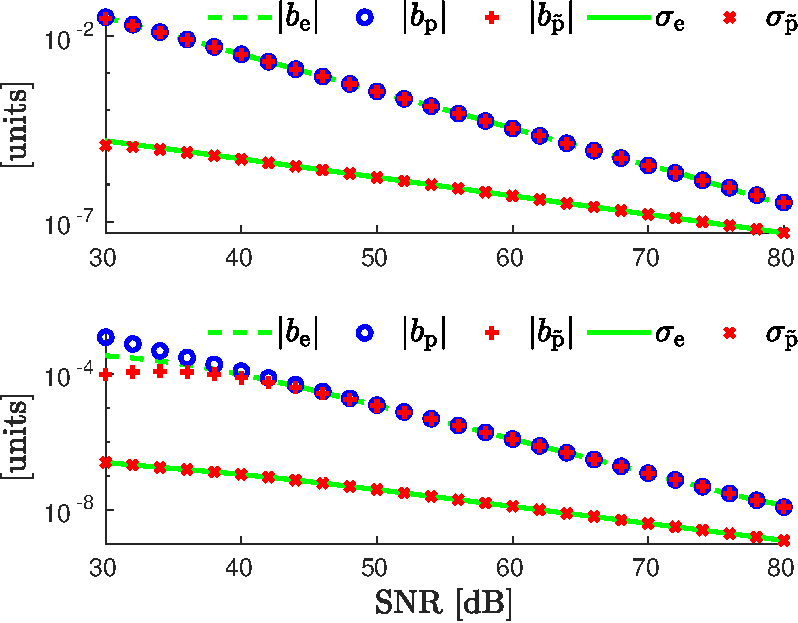
\includegraphics[width=1\columnwidth]{./ChapterStatisticalAnalysis/fig/Fig_1.pdf} 
  \caption{ \label{bias_sigma_NMC_unstr_str_n2} 
  We observe the results of the LS solutions for the unstructured (top) and the structured (bottom) EIV problems. These results are the empirical bias $b_{\mathrm{e}}$, the predicted bias from exact data $b_{\mathrm{p}}$, the predicted bias from observed data $b_{\widetilde{\mathrm{p}}}$, the empirical standard error $\sigma_{\mathrm{e}}$, and the standard error from the estimations using observed data $\sigma_{\widetilde{\mathrm{p}}}$. The estimation biases are proportional to the perturbation variance and the estimation standard errors are proportional to the perturbation standard deviation. Since the standard errors are smaller than the biases, the MC simulation is meaningful. }
\end{figure}

The absolute and relative errors between the predicted and the empirical bias are shown in Figure \ref{fig:b_bt_abse_rele_unstr_e7}. 
The absolute errors decrease with respect to the perturbation variance.
The relative errors are lower than 5\% for SNR between 30 dB and 70 dB. 
There is an increment in the relative errors for SNR above 55 dB. 
 As the SNR increases, the empirical and the predicted bias decrease, as well as the bias error between them.
In order to reveal the bias error, more Monte Carlo runs are needed to reduce the uncertainty of the Monte Carlo simulation that depends on the square root of $N_{\mathrm{MC}}$, see Equation (\ref{eqn:stderr}).
If $N_{\mathrm{MC}}$ is insufficient, the uncertainty of the Monte Carlo simulation hides the bias error and we see this increasing effect of the relative errors. 

\begin{figure}[htb!]
  \centering
  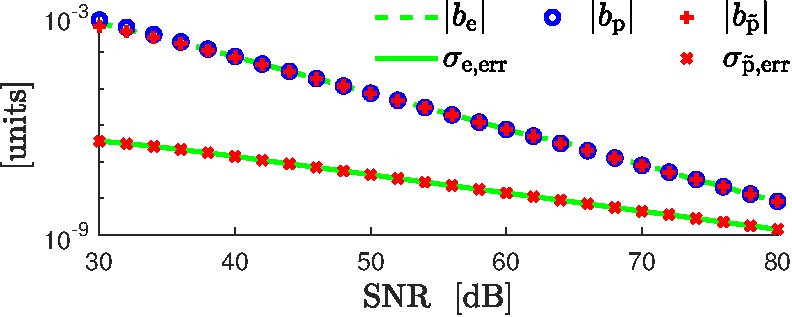
\includegraphics[width=1\columnwidth]{./ChapterStatisticalAnalysis/fig/Fig_2.pdf} 
  \caption{ \label{fig:b_bt_abse_rele_unstr_e7} The MC simulation shows that when we solve an unstructured EIV problem with LS, the absolute errors (top) between the predicted bias and the empirical bias are proportional to the perturbation noise variance as it is expected, and the relative errors (bottom) are smaller than 5\% for SNR below 70 dB. The bias prediction computed from exact data ${b}_\mathrm{p}$ is very similar to that computed using observed data $b_{\widetilde{\mathrm{p}}}$. } 
\end{figure}

The errors between the predicted and the empirical variance are shown in Figure \ref{fig:v_vt_abse_rele_unstr_e7}.
The absolute and relative errors decrease with respect to the perturbation variance.
The relative errors are lower than 5\% for SNR above 40 dB. 

\begin{figure}[htb!]
  \centering
  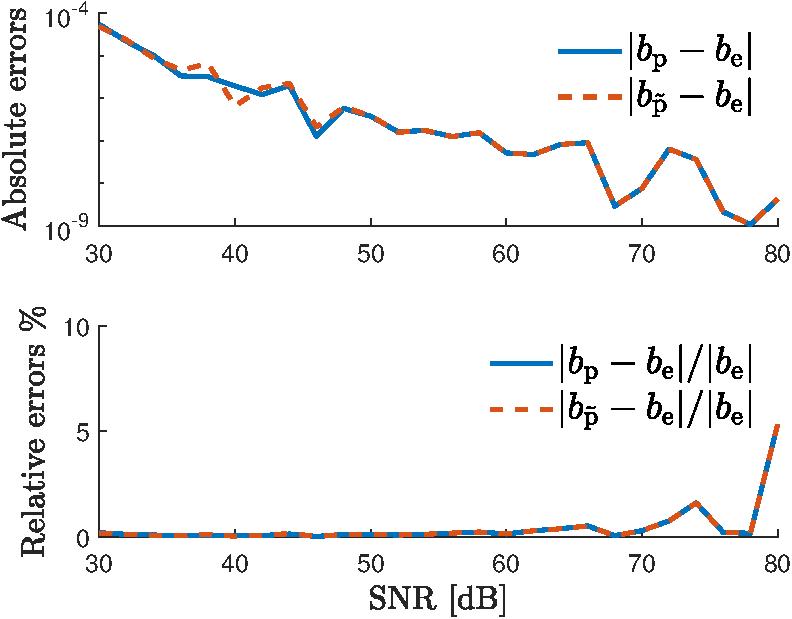
\includegraphics[width=1\columnwidth]{./ChapterStatisticalAnalysis/fig/Fig_3.pdf} 
  \caption{ \label{fig:v_vt_abse_rele_unstr_e7} The MC simulation shows that when we solve an unstructured EIV problem with LS, the absolute errors (top) between the predicted variances and the empirical variance are proportional to the perturbation noise variance, and the relative errors (bottom) are smaller than 5\% for SNR higher that 40 dB. The variance prediction computed using exact data ${v}_\mathrm{p}$ is very similar to that computed from observed data $v_{\widetilde{\mathrm{p}}}$. } 
\end{figure}

Figure \ref{fig:bv_btvt_abse_rele_unstr_e7} shows the absolute and the relative errors between the predictions computed from observed data and those computed from exact data.
The absolute errors between both predictions are proportional to the perturbation noise variance.
The bias and variance predictions, from either exact data or observed data, are equivalent for SNR above 35 dB since the relative errors are lower than 5\%.
The substitution of observed data on the prediction formulas is a valid procedure that allows the prediction of the estimate statistics.

\begin{figure}[htb!]
  \centering
  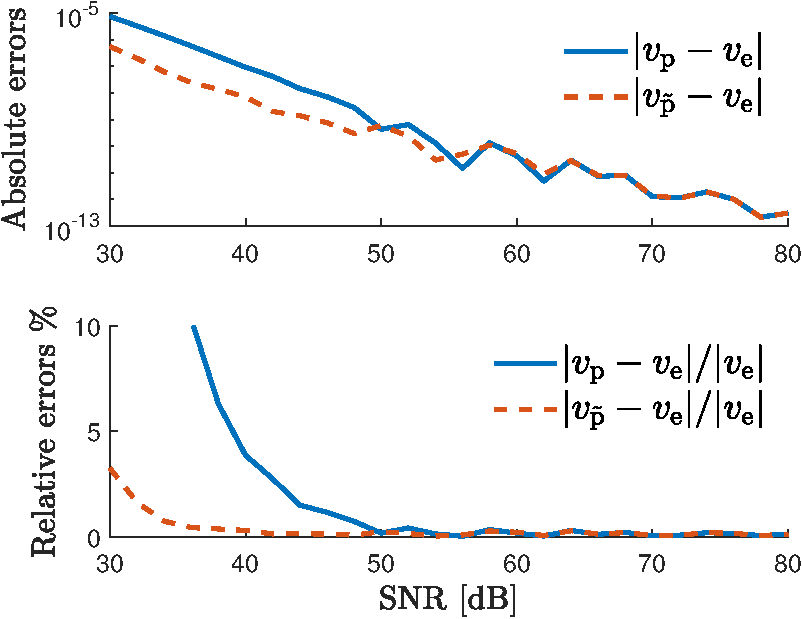
\includegraphics[width=1\columnwidth]{./ChapterStatisticalAnalysis/fig/Fig_4.pdf} 
  \caption{ \label{fig:bv_btvt_abse_rele_unstr_e7} The MC simulation shows that when we solve an unstructured EIV problem with LS, the absolute errors (top) between the prediction with observed data and the prediction with exact data are proportional to the perturbation noise variance. The use of observed data instead of exact data in the prediction formulas is valid when the SNR is above 35 dB since the relative errors (bottom) are smaller than 5\%. } 
\end{figure}


\subsection{Monte Carlo simulation results for a structured EIV problem with correlated perturbations}

The MC simulation of the structured EIV problem (\ref{eqn:ddsiemnd}) solution was conducted processing $T = 200$ samples of the transient response $\widetilde{\mathbf{y}}$ generated by a linear time invariant system of order $n = 2$, after a step input excitation with $u = 1 \ \mathrm{units}$, where the units represent any physical quantity. 
The processed step response is shown in Figure \ref{fig:y}.
The steady state response of the system is reached after 400 samples because from there on the relative error between the instantaneous values of the transient response and the steady-state response value is smaller than 2\%.
Processing 200 samples ensures that the step input estimation is computed from transient data only.
%In the following results we focus our interest in the first element of the estimate $\widehat{\mathbf{x}}_{\left[1\right]}$, where the step input level estimate $\widehat{u}$ is located.

\begin{figure}[htb!]
\centering
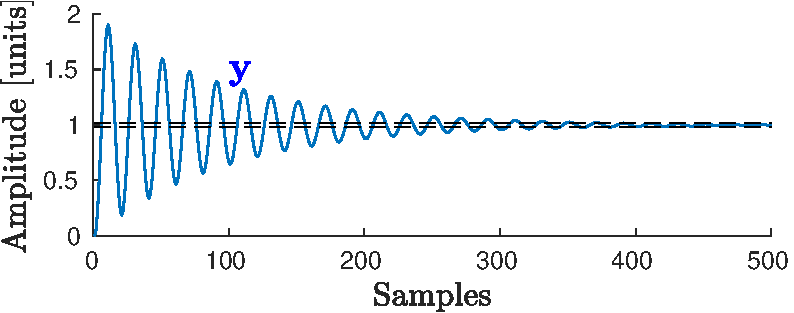
\includegraphics[width=1\columnwidth]{./ChapterStatisticalAnalysis/fig/Fig_5.pdf} 
\caption{ \label{fig:y} The structured EIV problem is constructed with 200 samples of the step response to ensure that only transient data is used. The relative errors between the values of $\mathbf{y}$ and the steady state value are smaller than 2\% after 400 samples, as it is indicated with dashed lines. } 
\end{figure}

The empirical bias is the sample mean of the $N_{\mathrm{MC}}$ estimates minus the true value
 \begin{equation} {b}_\mathrm{e} = \frac{1}{N_{\mathrm{MC}}} \sum_{i=1}^{N_{\mathrm{MC}}}{ \widehat{u}_i - u } \approx \mu \left( \widehat{u} \right) - u. \end{equation}
The standard error associated to this empirical bias estimation \citep{Hammersley75} is defined as 
\begin{equation} \sigma_\mathrm{e} = \frac{\sigma \left( \widehat{u} \right) }{\sqrt{N_{\mathrm{MC}}}}, \quad \mathrm{where} \quad \sigma^2 \left( \widehat{u} \right) = \frac{1}{N_{\mathrm{MC}}-1} \sum_{i=1}^{N_{\mathrm{MC}}}{ \left( { \widehat{u}}_i - \mu \left( \widehat{u} \right) \right)^2 } . \end{equation} 

The plots on the right side of Figure \ref{bias_sigma_NMC_unstr_str_n2} show the empirical bias, the bias predictions (\ref{eqn:biasE}) and (\ref{eqn:biasST}), and their corresponding standard errors, for the structured EIV problem.
The empirical bias $b_\mathrm{e}$ is proportional to the perturbation noise variance, and
the bias predictions $b_\mathrm{p}$ and $b_{\widetilde{\mathrm{p}}}$ coincide with the empirical bias $b_\mathrm{e}$ only for SNR above 40 dB.
This indicates that the SNR drops to a point where the constraint $\| \mathbf{M} \| < 1$ is no longer satisfied.
At an SNR of 30 dB the perturbation noise affects the bias prediction from observed data and it is three times smaller than the empirical bias.


The absolute and relative errors between the predicted and the empirical bias are shown in Figure \ref{fig:b_bt_abse_rele_str_e7}.
It can be seen that the absolute errors are proportional to the perturbation variance, and the relative errors are lower than 5\% for SNR higher than 40 dB. 
%Nevertheless, the perturbation SNR in practical applications is not high and is near 40 dB

\begin{figure}[htb!]
  \centering
  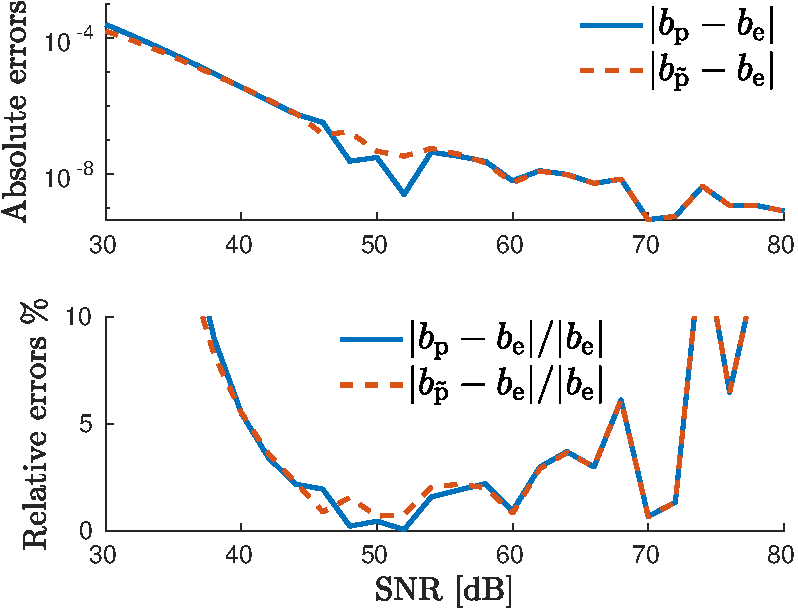
\includegraphics[width=1\columnwidth]{./ChapterStatisticalAnalysis/fig/Fig_6.pdf} 
  \caption{ \label{fig:b_bt_abse_rele_str_e7} The MC simulation shows that when we solve a structured EIV problem with LS, the absolute errors (top) between the predicted bias and the empirical bias $b_{\mathrm{e}}$ are proportional to the perturbation noise variance, and the relative errors (bottom) are smaller than 5\% only for SNR above 40 dB.}
\end{figure}


The absolute and relative errors between the empirical and the predicted variance, equations (\ref{eqn:varE}) and (\ref{eqn:varST}), are shown in Figure \ref{fig:v_vt_abse_rele_str_e7}.
These absolute errors are proportional to the perturbation noise variance, whereas
the relative errors are lower than 5\% for SNR higher than 45 dB. 

The absolute and relative errors between the two predictions from observed data and from exact data, are shown in Figure \ref{fig:bv_btvt_abse_rele_str_e7}.
These absolute errors are also proportional to the perturbation noise variance, and
the relative errors show that the bias and variance predictions from either of the two alternatives are equivalent for SNR higher than 45 dB.

\begin{figure}[htb!]
  \centering
  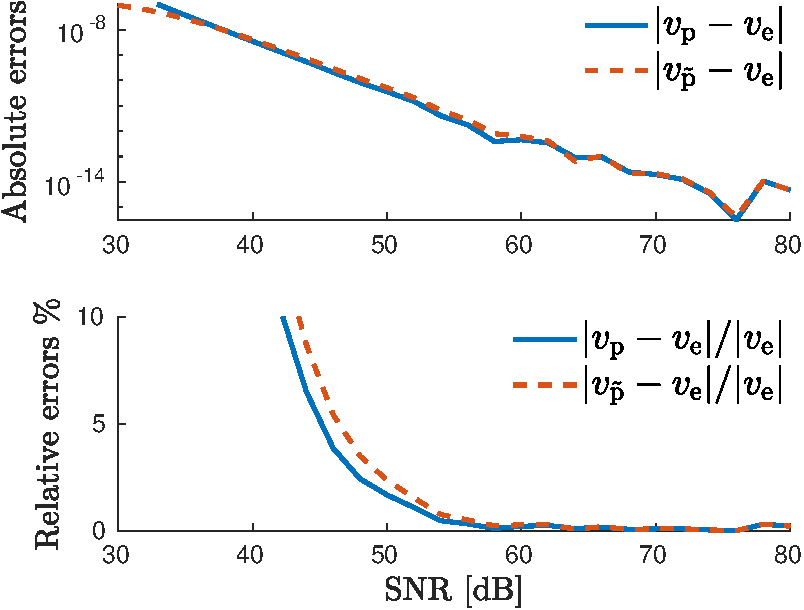
\includegraphics[width=1\columnwidth]{./ChapterStatisticalAnalysis/fig/Fig_7.pdf} 
  \caption{ \label{fig:v_vt_abse_rele_str_e7} The MC simulation shows that when we solve a structured EIV problem with LS, the absolute errors (top) between the predicted and the empirical variance are proportional to the perturbation variance, and the relative errors (bottom) between the predicted and the empirical variance are smaller than 5\% for SNR above 45 dB. }
\end{figure}

\begin{figure}[htb!]
  \centering
  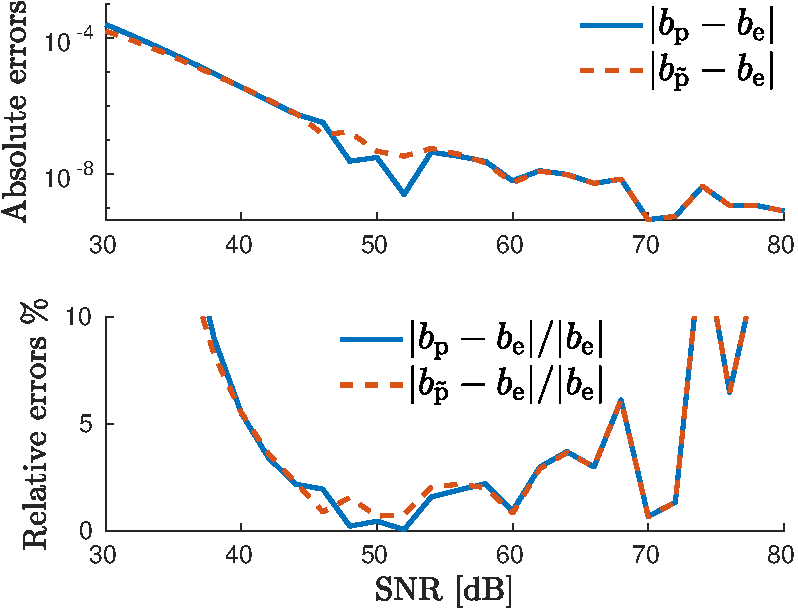
\includegraphics[width=1\columnwidth]{./ChapterStatisticalAnalysis/fig/Fig_8.pdf} 
  \caption{ \label{fig:bv_btvt_abse_rele_str_e7} The MC simulation shows that when we solve a structured EIV problem with LS, the absolute errors (top) between the predictions computed from observed data and those from exact data are proportional to the perturbation noise variance. According to the relative errors (bottom), the substitution is valid for SNR higher than 45 dB. } 
\end{figure}

The simulation results show that the LS solution of the structured and correlated EIV problem is more sensitive to the perturbation.
This represents a low limit in the SNR interval imposed by the noise level.
In practical applications it is common to have SNRs of 40 dB and the user needs to be aware of the prediction error that the method has.
We measure this prediction error with the mean squared error (MSE), defined as
\begin{equation} \mathrm{MSE} = \sigma^2 + b^2. \end{equation}
 By comparing the different MSEs to the CRLB of the structured EIV problem,
Figure \ref{fig:MSE_CRLB} shows that the MSEs has the same proportionality as the CRLB with respect to the disturbing noise variance.
The MSEs are three times larger than the CRLB.
Since the difference between $\mathrm{MSE}_{\widetilde{\mathrm{p}}}$ and the CRLB is lower than one order of magnitude, 
the LS estimation of the structured EIV problem produces results that are comparable to the ML estimation.
The $\mathrm{MSE}_{\widetilde{\mathrm{p}}}$ computed from observed data approaches the CRLB for SNR below 40 dB.
This is due to the constraint violation of the Taylor series expansion.


\begin{figure}[!htpb]
  \centering
  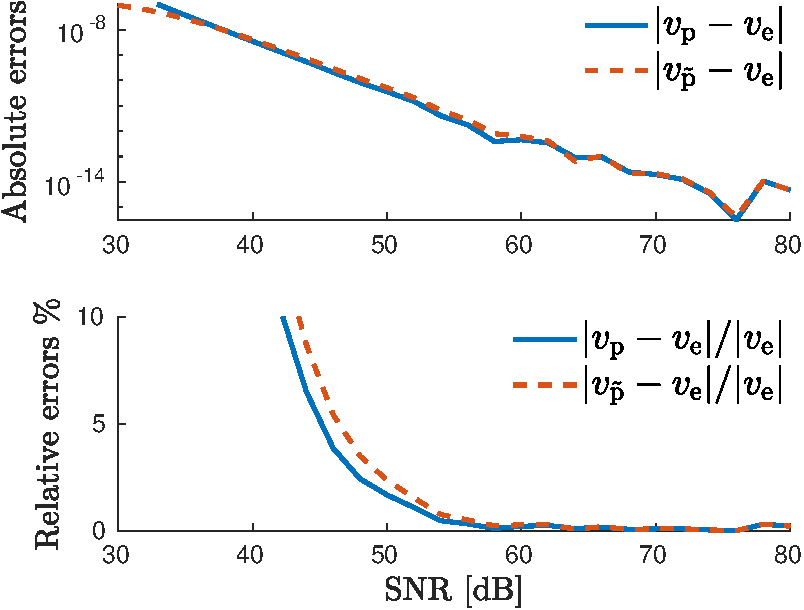
\includegraphics[width=1\columnwidth]{./ChapterStatisticalAnalysis/fig/Fig_9.pdf}
  \caption{\label{fig:MSE_CRLB}
The mean squared errors of the LS estimate are close to the Cram\'er-Rao lower bound. This is a positive indication of the goodness of the LS estimator for the structured EIV problem. The mean squared error of the empirical estimates is represented by $\mathrm{MSE}_{\mathrm{e}}$, and those of the predictions are $\mathrm{MSE}_{\mathrm{p}}$ and $\mathrm{MSE}_{\widetilde{\mathrm{p}}}$. The $\mathrm{MSE}_{\widetilde{\mathrm{p}}}$ is smaller than CRLB below 40 dB of SNR because of the introduced bias error, but the difference between $\mathrm{MSE}_{\widetilde{\mathrm{p}}}$ and the CRLB is lower than one order of magnitude.}
\end{figure}


\section{Conclusions}

 We conducted a statistical analysis of a structured errors-in-variables (EIV) estimation problem with correlation to find the first and second moments of its least-squares solution.
This estimation problem occurs in metrology when we estimate the value of a measurand directly from the sensor transient response.
The data-driven estimation of the physical quantity is formulated as a structured EIV problem with correlation that uses the observed transient response to construct both the regression matrix and the regressor.
The real-time implementation of the method uses a recursive least squares algorithm that is simple and has low computational complexity.
The assessment of the uncertainty is done using the estimate bias and variance.

The conducted statistical analysis produced expressions that predict the estimate bias and variance for given sample size and perturbation level of the observed response.
The Monte Carlo simulation validated the predictions.
We compared the results of solving an unstructured and uncorrelated EIV problem with a structured and correlated EIV problem to understand how the structure and the correlation impacts in the estimation.
We found that the predictions in the structured case are more susceptible to perturbations.
This is due to the two approximations involved, a second-order Taylor series expansion of the estimate, and the substitution of perturbed data on the prediction expressions.
The relative error results indicate that the estimate bias, and variance are predicted using the derived expressions, and the observed data.
The mean squared error of the estimate is close to the results of the maximum likelihood estimate given by the Cram\'er-Rao lower bound.

The bias and variance can be accurately predicted, provided that the Taylor series expansion is valid.
This constraint has to be taken into account to ensure the effectiveness of the method in practical applications.
In the example, it was observed that when the SNR lies outside the validity region, the bias and variance estimation was at most three times larger than the empirical values.

The methodology presented in this paper can be applied to estimate the uncertainty of the solutions to other structured EIV problems.
The bias and variance expressions obtained after the statistical analysis depend on each specific structure.



\begin{comment}

\section{STATISTICAL ANALYSIS - Ramp input}


\subsubsection{Statistical analysis of the subspace method}

To obtain the first and second moments of the step input estimate $\widehat{u}$, we need to study the solution
\begin{equation} \widehat{\mathbf{x}} = ( \mathbf{K}^\top \mathbf{W} \mathbf{K}  )^{-1} \mathbf{K}^\top \mathbf{W} \mathbf{y} , \label{eqn:xhat} \end{equation}
of the overdetermined structured errors-in-variables EIV problem (\ref{eqn:min_ewrls}).
Using a second order Taylor series expansion of the inverse matrix we can approximate the LS solution as
\begin{equation} \widehat{\mathbf{x}} \approx \left( \mathbf{I} - \mathbf{M} + \mathbf{M}^2 \right) \mathbf{C}^{-1} (\widebar{\mathbf{K}} + \mathbf{E})^\top \mathbf{W} (\widebar{\mathbf{y}} + \bm{\epsilon}). \label{eqn:xhatexp} \end{equation} 
where 
\begin{equation} \widebar{\mathbf{C}} = \widebar{\mathbf{K}}^\top \mathbf{W} \widebar{\mathbf{K}}, \quad \text{and} \quad \mathbf{M} = \widebar{\mathbf{C}}^{-1} ( \widebar{\mathbf{K}}^\top \mathbf{W} \mathbf{E} + \mathbf{E}^\top \mathbf{W} \widebar{\mathbf{K}} + \mathbf{E}^\top \mathbf{W} \mathbf{E} ). \end{equation} 

The Taylor series approximation of $\widehat{\mathbf{x}}$ enables the calculation of the estimate bias and covariance since the measurement noise $\bm{\epsilon}$ and $\mathbf{E}$ are no more subject to matrix inversion. 
The bias and the covariance of the estimate $\widehat{\mathbf{x}}$ are obtained from
\begin{equation}  \mathbf{b} \left(\widehat{\mathbf{x}} \right) = \mathbf{\mu} - \widebar{\mathbf{x}}, \label{eqn:biasdef} \end{equation}
\begin{equation} \begin{aligned} \mathrm{\mathbf{Cov}} \left( \widehat{\mathbf{x}} \right) & = \mathbb{E} \left\{ \left( \widehat{\mathbf{x}} - \mathbf{\mu} \right)  \left( \widehat{\mathbf{x}} - \mathbf{\mu} \right)^\top \right\} . \end{aligned} \label{eqn:covdef} \end{equation} 
where $\mathbf{\mu} = \mathbb{E} \left\{ \widehat{\mathbf{x}} \right\}$ is the expected value of the estimate and $\widebar{\mathbf{x}}$ is the true value. 
Considering the structure of the EIV problem, the bias and the covariance of the estimate approximation (\ref{eqn:xhatexp}) can be expressed as
\begin{equation} \begin{aligned} \widebar{\mathbf{b}}_{\mathrm{p}} \left( \widehat{x} \right) & \approx \widebar{\mathbf{C}}^{-1} \left(  \left( \widebar{\mathbf{K}}^\top \mathbf{W} \widebar{\mathbf{B}}_1 - \widebar{\mathbf{B}}_2 \right) \mathbf{x} - \left( \widebar{\mathbf{K}}^\top \mathbf{W} \widebar{\mathbf{B}}_3 - \widebar{\mathbf{B}}_4 \right) \right), \end{aligned} \label{eqn:biasE} \end{equation}
\begin{equation} \begin{aligned} \widebar{\mathrm{\mathbf{Cov}}}_{\mathrm{p}} \left( \widehat{\mathbf{x}} \right) & \approx \widebar{\mathbf{K}}^\dagger \mathbf{W} \left( \sigma_{\epsilon}^2 \mathbf{I}_{T-n} + \widebar{\mathbf{C}}_1 - \widebar{\mathbf{C}}_2 - \widebar{\mathbf{C}}_2^\top \right) \mathbf{W} \widebar{\mathbf{K}}^{\dagger \top}  - \widebar{\mathbf{b}}_{\mathrm{p}} \left( \widehat{x} \right) \widebar{\mathbf{b}}_{\mathrm{p}}^\top \left( \widehat{x} \right), \end{aligned} \label{eqn:varE} \end{equation}
where $\widebar{\mathbf{B}}_1 = \mathbb{E} \Big\{ \mathbf{E} \widebar{\mathbf{K}}^\dagger \mathbf{W} \mathbf{E} \Big\}$, $\widebar{\mathbf{B}}_2 = \mathbb{E} \Big\{ \mathbf{E}^\top \mathbf{W} \widebar{\mathbf{P}}_\perp \mathbf{E} \Big\}$, $\widebar{\mathbf{B}}_3 = \mathbb{E} \Big\{ \mathbf{E} \widebar{\mathbf{K}}^\dagger \mathbf{W} \bm{\epsilon} \Big\}$, $\widebar{\mathbf{B}}_4 = \mathbb{E} \Big\{ \mathbf{E}^\top \mathbf{W} \widebar{\mathbf{P}}_\perp \bm{\epsilon} \Big\}$, $\widebar{\mathbf{C}}_1 = \mathbb{E} \Big\{ \mathbf{E} \mathbf{x} \mathbf{x}^\top \mathbf{E}^\top \Big\}$, \linebreak $\widebar{\mathbf{C}}_2 = \mathbb{E} \Big\{ \mathbf{E} \mathbf{x} \bm{\epsilon}^\top \Big\}$, $\widebar{\mathbf{P}}_\perp = \mathbf{I} - \widebar{\mathbf{K}} \widebar{\mathbf{K}}^\dagger \mathbf{W}$, and $\mathbf{K}^\dagger$ is the pseudo-inverse matrix of $\mathbf{K}$. 

The bias and covariance given by expressions (\ref{eqn:biasE}) and (\ref{eqn:varE}) depend on the unobservable true values $\widebar{\mathbf{x}}$ and $\widebar{\mathbf{K}}$.
The measured observations are in the sensor step response $\mathbf{y}$, and from its observations we construct $\mathbf{K}$ and compute $\widehat{\mathbf{x}}$.
The substitution of the measured data in the expressions gives an approximation of the estimate bias and covariance. 
We have then
\begin{equation} \begin{aligned} \mathbf{b}_{\mathrm{p}} \left( \widehat{\mathbf{x}} \right) & \approx \mathbf{C}^{-1} \left(  \left( \mathbf{K}^\top \mathbf{W} \mathbf{B}_1 - \mathbf{B}_2 \right) \widehat{\mathbf{x}} - \left( \mathbf{K}^\top \mathbf{W} \mathbf{B}_3 - \mathbf{B}_4 \right) \right), \end{aligned} \label{eqn:biasST} \end{equation}
  \begin{equation} \begin{aligned} {\mathrm{\mathbf{Cov}}}_{\mathrm{p}} \left( \widehat{\mathbf{x}} \right) & \approx \mathbf{K}^\dagger \mathbf{W} \left( \sigma_{\epsilon}^2 \mathbf{I}_{T-n} + \mathbf{C}_1 - \mathbf{C}_2 - \mathbf{C}_2^\top \right) \mathbf{W} \mathbf{K}^{\dagger \top} - \mathbf{b}_{\mathrm{p}} \left( \widehat{x} \right) \mathbf{b}_{\mathrm{p}}^\top \left( \widehat{x} \right), \end{aligned} \label{eqn:varST} \end{equation}
  where $\mathbf{B}_1 = \mathbb{E} \Big\{ \mathbf{E} \mathbf{K}^\dagger \mathbf{W} \mathbf{E} \Big\}$, $\mathbf{B}_2 = \mathbb{E} \Big\{ \mathbf{E}^\top \mathbf{W} \mathbf{P}_\perp \mathbf{E} \Big\}$, $\mathbf{B}_3 = \mathbb{E} \Big\{ \mathbf{E} \mathbf{K}^\dagger \mathbf{W} \bm{\epsilon} \Big\}$, $\mathbf{B}_4 = \mathbb{E} \Big\{ \mathbf{E}^\top \mathbf{W} \mathbf{P}_\perp \bm{\epsilon} \Big\}$, $\mathbf{C}_1 = \mathbb{E} \Big\{ \mathbf{E} \widehat{\mathbf{x}} \widehat{\mathbf{x}}^\top \mathbf{E}^\top \Big\}$, $\mathbf{C}_2 = \mathbb{E} \Big\{ \mathbf{E} \widehat{\mathbf{x}} \bm{\epsilon}^\top \Big\}$, and $\mathbf{P}_\perp = \mathbf{I} - \mathbf{K} \mathbf{K}^\dagger \mathbf{W}$. 

  The results of the expected values $\mathbf{B}_1$, $\mathbf{B}_2$, $\mathbf{B}_3$, $\mathbf{B}_4$, $\mathbf{C}_1$, and $\mathbf{C}_2$, were described by the authors of this paper in \citep{Quintana19}.
The bias and covariance were obtained to extend previous analysis conducted on EIV estimation problems without an imposed structure \citep{Vaccaro94, Stewart90SPT}.
It was shown that the bias and variance expressions (\ref{eqn:biasST}) and (\ref{eqn:varST}) are valid predictions of the first and second moments of the LS estimate of a Hankel structured EIV problem.
The problem formulated by the step input estimation method belongs to this type of structured EIV problems and can use the derived expressions to find the bias and variance of the input estimate $\widehat{u}$.
The bias of the estimate $\widehat{u}$ is the fist element of $\mathbf{b}_{\mathrm{p}} \left( \widehat{\mathbf{x}} \right)$ and the variance of $\widehat{u}$ is the first element in the main diagonal of $\mathrm{\mathbf{Cov}}_{\mathrm{p}} \left( \widehat{\mathbf{x}} \right)$.


\subsubsection{Cram\'er-Rao lower bound of the structured EIV problem}

To find the Cram\'er-Rao lower bound (CRLB) of the structured EIV estimation problem (\ref{eqn:min_ls}), we consider that this structured and correlated estimation problem can be expressed as a linear in the measurements problem \citep{Pintelon12Book}
\begin{equation} e (\widehat{\mathbf{x}}, \mathbf{z}) = \mathbf{M}_1( \widehat{\mathbf{x}} ) \ \mathbf{z} = \underbrace{\begin{bmatrix} \mathbf{I}_{T-n} & - \widehat{\mathbf{x}}^T \otimes \mathbf{I}_{T-n} \end{bmatrix}}_{\mathbf{M}_1( \widehat{\mathbf{x}} )} \underbrace{\begin{bmatrix} \mathbf{y} \\ \mathrm{vec} ( \mathbf{K} ) \end{bmatrix}}_{\mathbf{z}} = 0 . \label{eqn:M1vecyK} \end{equation}
where $\mathbf{z} = \widebar{\mathbf{z}} + \bm{\epsilon}_{\mathbf{z}}$.
To have the CRLB, it is necessary the existence of the true model $\mathbf{M}_1( \mathbf{x} ) \ \mathbf{z} = 0$.
The measurement perturbation $\bm{\epsilon}_{\mathbf{z}}$ is assumed to be normally distributed with covariance matrix $\mathbf{C}_{\mathbf{z}}$, and then, the loglikelihood function of the structured and correlated EIV problem is
\begin{equation} \ln{ l(\mathbf{z}, \widehat{\mathbf{z}}, \widehat{\mathbf{x}}) } = - \frac{1}{2} \left( \mathbf{z} - \widehat{\mathbf{z}} \right)^\top \mathbf{C}_{\mathbf{z}}^{-1} \left( \mathbf{z} - \widehat{\mathbf{z}} \right) + \mathrm{constant}, \end{equation}
where the elements of $\widehat{\mathbf{z}}$ are the estimated parameters of the measurements $\mathbf{z}$,  that satisfy $\mathbf{M}_1(\widehat{\mathbf{x}}) \ \widehat{\mathbf{z}} = 0$.
The size of the Fisher information matrix $\mathbf{Fi}(\mathbf{x}, \mathbf{z})$ depends on the number of unknowns in $\widehat{\mathbf{z}}$ and grows with the sample size.
However, the Fisher information matrix $\mathbf{Fi}(\mathbf{x})$ is obtained from $\mathbf{Fi}(\mathbf{x}, \mathbf{z})$, by doing inversion by parts \citep{Pintelon12Book} \S 19, and can be expressed as  
\begin{equation} \mathbf{Fi}(\mathbf{x}) = \left( \frac{\partial e (\widehat{\mathbf{x}}, \mathbf{z}) }{\partial \mathbf{x} } \right)^\top \left( \mathbf{M}_1( \mathbf{x} ) \mathbf{C}_{\mathbf{z}}  \mathbf{M}_1^\top( \mathbf{x} ) \right)^{-1}  \left( \frac{\partial e (\widehat{\mathbf{x}}, \mathbf{z}) }{\partial \mathbf{x} } \right) .
 \label{eqn:FIM}   \end{equation} 
The partial derivatives are evaluated at the true values $\mathbf{x}$. 
Thus, the covariance matrix of the measurements is

\begin{equation} \mathbf{C}_{\mathbf{z}} = \sigma_{\epsilon}^2 \begin{bmatrix} \mathbf{I}_{T-n} & \mathbf{0}_{T-n} & \mathbf{D}_1 \\ \mathbf{0}_{T-n} & \mathbf{0}_{T-n} & \mathbf{0}_{T-n \times n \left( T-n \right)}  \\  \mathbf{D}_1^\top & \mathbf{0}_{n \left( T-n \right) \times T-n} & \mathbf{D}_2  \end{bmatrix}  \label{eqn:Cz} \end{equation} 
where
\begin{equation*} \begin{aligned} \mathbf{D}_1 &= \begin{bmatrix}\mathbf{D}_{T-n \times T-n}^{1,n} & \mathbf{D}_{T-n \times T-n}^{1,n-1} & \cdots  & \mathbf{D}_{T-n \times T-n}^{1,1}\end{bmatrix}, \\ 
 \mathbf{D}_2 &= \begin{bmatrix} \mathbf{D}_{T-n \times T-n}^{2,1} & \mathbf{D}_{T-n \times T-n}^{2,0} & \cdots & \mathbf{D}_{T-n \times T-n}^{2,2-n} \\ \mathbf{D}_{T-n \times T-n}^{2,2} & \mathbf{D}_{T-n \times T-n}^{2,1} & \cdots & \mathbf{D}_{T-n \times T-n}^{2,3-n} \\ \vdots & \vdots & & \vdots \\ \mathbf{D}_{T-n \times T-n}^{2,n} & \mathbf{D}_{T-n \times T-n}^{2,n-1} & \cdots & \mathbf{D}_{T-n \times T-n}^{2,1} \end{bmatrix} , \end{aligned}  \end{equation*} 
and the matrices
$\mathbf{D}_{r \times c}^{1,k}$ and $\mathbf{D}_{r \times c}^{2,k}$  are the first and second order finite differences matricial operators of dimensions $r \times c$  starting from the subdiagonal $k$, for example \begin{equation*} 
\mathbf{D}_{2 \times 3}^{1,1} = \begin{bmatrix} 1 & -1 & 0 \\ 0 & 1 & -1 \end{bmatrix}, \ \mathrm{and} \quad \mathbf{D}_{3 \times 3}^{2,0} = \begin{bmatrix}-1 & 0 & 0 \\ 2 & -1 & 0 \\ - 1 & 2 & -1  \end{bmatrix} . \end{equation*}
 
The Cram\'er-Rao lower bound for a biased estimator of the minimization problem (\ref{eqn:min_ls}) is 
\begin{equation} \mathrm{CRLB}_{\mathrm{b}}(\mathbf{x}) = \left( \mathbf{I}_{n+1} + \frac{\partial \mathbf{b} \left( \widehat{\mathbf{x}} \right) }{\partial \mathbf{x} } \right)^\top \mathbf{Fi}^{-1}(\mathbf{x}) \left( \mathbf{I}_{n+1} + \frac{\partial \mathbf{b} \left( \widehat{\mathbf{x}} \right) }{\partial \mathbf{x} } \right), \label{eqn:CRB_EIV} \end{equation} 
whereas for an unbiased estimator, it is $\mathrm{CRLB}_{\mathrm{ub}}(\mathbf{x}) = \mathbf{Fi}^{-1}(\mathbf{x})$.





\section{STATISTICAL ANALYSIS - Experimental validation}

To obtain the first and second moments of the step input estimate $\widehat{u}$, we need to study the least-squares (LS) solution 
\begin{equation} \widehat{\mathbf{x}} = \widetilde{\mathbf{K}}^\dagger \widetilde{\mathbf{y}} = ( \widetilde{\mathbf{K}}^\top \widetilde{\mathbf{K}}  )^{-1} \widetilde{\mathbf{K}}^\top \widetilde{\mathbf{y}} , \label{eqn:xhat} \end{equation}
of the overdetermined structured errors-in-variables EIV problem (\ref{eqn:min_ls}), 
where $\widetilde{\mathbf{K}}^\dagger$ is the pseudo-inverse matrix of $\widetilde{\mathbf{K}}$.
Using a second order Taylor series expansion of the inverse matrix we can approximate the LS solution as
\begin{equation} \widehat{\mathbf{x}} \approx \left( \mathbf{I} - \mathbf{M} + \mathbf{M}^2 \right) \mathbf{Q}^{-1} (\mathbf{K}+\mathbf{E})^\top (\mathbf{y}+\bm{\epsilon}). \label{eqn:xhatexp} \end{equation} 
where 
\begin{equation} \mathbf{Q} = \mathbf{K}^\top \mathbf{K}, \quad \text{and} \quad \mathbf{M} = \mathbf{Q}^{-1} ( \mathbf{K}^\top \mathbf{E} + \mathbf{E}^\top \mathbf{K} + \mathbf{E}^\top \mathbf{E} ). \end{equation} 

The Taylor series approximation of $\widehat{\mathbf{x}}$ enables the calculation of the bias and covariance of $\widehat{\mathbf{x}}$ since the measurement noise $\bm{\epsilon}$ and $\mathbf{E}$ are no more subject to matrix inversion. 
The bias and the covariance of the estimate $\widehat{\mathbf{x}}$ are obtained from
\begin{equation}  \mathbf{b} \left(\widehat{\mathbf{x}} \right) = \mathbf{\mu} - \mathbf{x}, \label{eqn:biasdef} \end{equation}
\begin{equation} \begin{aligned} \mathrm{\mathbf{C}} \left( \widehat{\mathbf{\mathbf{x}}} \right) & = \mathbb{E} \left\{ \left( \widehat{\mathbf{x}} - \mathbf{\mu} \right)  \left( \widehat{\mathbf{x}} - \mathbf{\mu} \right)^\top \right\} . \end{aligned} \label{eqn:covdef} \end{equation} 
where $\mathbf{\mu} = \mathbb{E} \left\{ \widehat{\mathbf{x}} \right\}$, and $\mathbf{x} = \mathbf{K}^\dagger \mathbf{y}$ is the true value. 
Considering the structure of the EIV problem, the bias and the covariance of the approximation (\ref{eqn:xhatexp}) can be expressed as
\begin{equation} \begin{aligned} \mathbf{b}_{\mathrm{p}} \left( \widehat{\mathbf{x}} \right) & \approx \mathbf{Q}^{-1} \left(  \left( \mathbf{K}^\top \mathbf{B}_1 - \mathbf{B}_2 \right) \mathbf{x} - \left( \mathbf{K}^\top \mathbf{B}_3 - \mathbf{B}_4 \right) \right), \end{aligned} \label{eqn:biasE} \end{equation}
\begin{equation} \begin{aligned} \mathrm{\mathbf{C}}_{\mathrm{p}} \left( \widehat{\mathbf{x}} \right) & \approx \mathbf{K}^\dagger \left( \sigma_{\bm{\epsilon}}^2 \mathbf{I}_{T-n} + \mathbf{C}_1 - \mathbf{C}_2 - \mathbf{C}_2^\top \right) \mathbf{K}^{\dagger \top}, \end{aligned} \label{eqn:varE} \end{equation}
where $\mathbf{B}_1 = \mathbb{E} \Big\{ \mathbf{E} \mathbf{K}^\dagger \mathbf{E} \Big\}$, $\mathbf{B}_2 = \mathbb{E} \Big\{ \mathbf{E}^\top \mathbf{P}_\perp \mathbf{E} \Big\}$, $\mathbf{B}_3 = \mathbb{E} \Big\{ \mathbf{E} \mathbf{K}^\dagger \bm{\epsilon} \Big\}$, $\mathbf{B}_4 = \mathbb{E} \Big\{ \mathbf{E}^\top \mathbf{P}_\perp \bm{\epsilon} \Big\}$, $\mathbf{C}_1 = \mathbb{E} \Big\{ \mathbf{E} \mathbf{x} \mathbf{x}^\top \mathbf{E}^\top \Big\}$, \linebreak $\mathbf{C}_2 = \mathbb{E} \Big\{ \mathbf{E} \mathbf{x} \bm{\epsilon}^\top \Big\}$, and $\mathbf{P}_\perp = \mathbf{I} - \mathbf{K} \mathbf{K}^\dagger$. 

The expected values $\mathbf{B}_1$, $\mathbf{B}_2$, $\mathbf{B}_3$, $\mathbf{B}_4$, $\mathbf{C}_1$, and $\mathbf{C}_2$, were studied in \citep{Quintana19} and their results are described in Lemma \ref{lem:lemma1}:


% \normalsize % \small
%   <how to set font size here to 10 px ? />

\begin{lem}
Let $\mathbf{E}$ be the matrix defined in (\ref{eqn:matrixE}),
constructed from samples of the i.i.d. normally distributed random variable $\bm{\epsilon} \sim \mathcal{N}(0, \sigma_\epsilon^2)$.
For a compatible deterministic matrix $\mathbf{H}$, or vector $\mathbf{h}$, we have
\begin{equation*} \begin{aligned} 
& \mathbb{E} \left\{ \mathbf{E} \mathbf{H} \mathbf{E} \right\} = \sigma_{\bm{\epsilon}}^2 \mathbf{A}, \
\text{where} \ a_{ij} = \mathrm{tr} \left( \mathbf{H} \begin{bmatrix} 0_{T-n} & \mathbf{D}_{T-n \times n}^{2, j-i} \end{bmatrix} \right), \\
& \ \ \text{for}  \ i = 1, \cdots, T-n, \ \text{and} \ j = 2, \cdots, n+1, \ \text{and} \ a_{i1} = 0. \\
& \mathbb{E} \left\{ \mathbf{E}^\top \mathbf{H} \mathbf{E} \right\} = \sigma_{\bm{\epsilon}}^2 \mathbf{A}, \ 
\text{where} \ a_{ij} = \mathrm{tr} \left( \mathbf{H} \ \mathbf{D}_{T-n \times T-n}^{2, j-i+1} \right)  , \\
& \ \ \text{for} \ i = 2, \cdots, n+1, \ \text{and} \ j=2, \cdots, n+1 , \ \text{and} \   a_{1j} = a_{i1} = 0,  \\ 
& \mathbb{E} \left\{ \mathbf{E} \mathbf{H} \mathbf{E}^\top \right\} = \sigma_{\bm{\epsilon}}^2 \mathbf{A}, \
\text{where} \ a_{ij} = \mathrm{tr} \left( \mathbf{H} \begin{bmatrix} 0 & 0_{n}^\top \\ 0_{n} & \mathbf{D}_{n \times n}^{2, j-i+1} \end{bmatrix} \right), \\
& \ \ \text{for} \ i = 1,\cdots,T-n, \ \text{and} \ j=1,\cdots,T-n. \\ 
& \mathbb{E} \left\{ \mathbf{E} \mathbf{H} \bm{\epsilon} \right\} = \sigma_{\bm{\epsilon}}^2 \mathbf{a} , \
\text{where} \ a_i = \mathrm{tr} \left( \mathbf{H} \begin{bmatrix} 0_{T-n} & \mathbf{D}_{T-n \times n}^{1,n+1-i} \end{bmatrix} \right) , \\
& \ \ \text{for} \ i = 1,\cdots,T-n . \\
& \mathbb{E} \left\{ \mathbf{E}^\top \mathbf{H} \bm{\epsilon} \right\} = \sigma_{\bm{\epsilon}}^2 \mathbf{a}, \
\text{where} \ a_i = \ \mathrm{tr} \left( \mathbf{H} \ \mathbf{D}_{T-n \times T-n}^{1, n+2-i} \right), \\ & \ \ \text{for} \ i = 2,\cdots,n+1  , \ \text{and} \ a_1 = 0,   \\
& \mathbb{E} \left\{ \mathbf{E} \mathbf{h} \bm{\epsilon}^\top \right\} = \sigma_{\bm{\epsilon}}^2 \mathbf{Z}, \
\text{where} \ \mathbf{Z}_{j} = -\mathbf{D}_{T-n \times n+1}^{1,-j} \begin{bmatrix} & \mathbf{R}_n \\ 0 \end{bmatrix} \mathbf{h} ,  \\ 
& \ \ \text{for} \ j = 1,\cdots,T-n ,\\
\end{aligned} \end{equation*} 
where $\mathbf{R}_n$ is a reversal matrix, and the matrices
$\mathbf{D}_{r \times c}^{1,k}$ and $\mathbf{D}_{r \times c}^{2,k}$  are the first and second order finite differences matricial operators of dimensions $r \times c$  starting from the subdiagonal $k$, for example \begin{equation*} 
\mathbf{D}_{2 \times 3}^{1,1} = \begin{bmatrix} 1 & -1 & 0 \\ 0 & 1 & -1 \end{bmatrix}, \ \text{and} \quad \mathbf{D}_{3 \times 3}^{2,0} = \begin{bmatrix}-1 & 0 & 0 \\ 2 & -1 & 0 \\ - 1 & 2 & -1  \end{bmatrix} .
\end{equation*} 
\end{lem}

\normalsize

A proof of the lemma is given in the Appendix.

The bias and covariance given by expressions (\ref{eqn:biasE}) and (\ref{eqn:varE}) depend on the unobservable true values $\mathbf{x}$, $\mathbf{K}$.
The measured variable is the sensor step response $\widetilde{\mathbf{y}}$, and from its observations we construct $\widetilde{\mathbf{K}}$ and compute $\widehat{\mathbf{x}}$.
The substitution of the measured data in the expressions gives an approximation of the bias and covariance estimation.
We have then
\begin{equation} \begin{aligned} \mathbf{b}_{\widetilde{\mathrm{p}}} \left( \widehat{\mathbf{x}} \right) & \approx \widetilde{\mathbf{Q}}^{-1} \left(  \left( \widetilde{\mathbf{K}}^\top \widetilde{\mathbf{B}}_1 - \widetilde{\mathbf{B}}_2 \right) \widehat{\mathbf{x}} - \left( \widetilde{\mathbf{K}}^\top \widetilde{\mathbf{B}}_3 - \widetilde{\mathbf{B}}_4 \right) \right), \end{aligned} \label{eqn:biasST} \end{equation}
\begin{equation} \begin{aligned} \mathrm{\mathbf{C}}_{\widetilde{\mathrm{p}}} \left( \widehat{\mathbf{x}} \right) & \approx \widetilde{\mathbf{K}}^\dagger \left( \sigma_{\epsilon}^2 \mathbf{I}_{T-n} + \widetilde{\mathbf{C}}_1 - \widetilde{\mathbf{C}}_2 - \widetilde{\mathbf{C}}_2^\top \right) \widetilde{\mathbf{K}}^{\dagger \top}, \end{aligned} \label{eqn:varST} \end{equation}
where $\widetilde{\mathbf{B}}_1 = \mathbb{E} \Big\{ \mathbf{E} \widetilde{\mathbf{K}}^\dagger \mathbf{E} \Big\}$, $\widetilde{\mathbf{B}}_2 = \mathbb{E} \Big\{ \mathbf{E}^\top \widetilde{\mathbf{P}}_\perp \mathbf{E} \Big\}$, $\widetilde{\mathbf{B}}_3 = \mathbb{E} \Big\{ \mathbf{E} \widetilde{\mathbf{K}}^\dagger \bm{\epsilon} \Big\}$, $\widetilde{\mathbf{B}}_4 = \mathbb{E} \Big\{ \mathbf{E}^\top \widetilde{\mathbf{P}}_\perp \bm{\epsilon} \Big\}$, $\widetilde{\mathbf{\mathbf{C}}}_1 = \mathbb{E} \Big\{ \mathbf{E} \widehat{\mathbf{x}} \widehat{\mathbf{x}}^\top \mathbf{E}^\top \Big\}$, $\widetilde{\mathbf{C}}_2 = \mathbb{E} \Big\{ \mathbf{E} \widehat{\mathbf{x}} \bm{\epsilon}^\top \Big\}$, and $\widetilde{\mathbf{P}}_\perp = \mathbf{I} - \widetilde{\mathbf{K}} \widetilde{\mathbf{K}}^\dagger$. 

The bias and covariance were obtained to extend previous analysis conducted on EIV estimation problems without an imposed structure \citep{Vaccaro94, Stewart90SPT}.
It was shown that the bias and variance expressions (\ref{eqn:biasST}) and (\ref{eqn:varST}) are good predictions of the first and second moments of the LS estimate of a Hankel structured EIV problem.
The problem formulated by the step input estimation method belongs to this type of structured EIV problems and the derived expressions can be used to find the bias and variance of the input estimate $\widehat{u}$.
The bias and variance predictions approximate the empirical bias and variance.

The assessment of the uncertainty of the estimate $\widehat{\mathbf{x}}$ is obtained from the covariance matrix $\mathrm{\mathbf{C}}_{\widetilde{\mathrm{p}}} \left( \widehat{\mathbf{x}} \right)$. In this way, the uncertainty of the step input estimate $\widehat{u}$ is described by the variance in the first element on the diagonal of $\mathrm{\mathbf{C}}_{\widetilde{\mathrm{p}}} \left( \widehat{\mathbf{x}} \right)$.

In the rest of this section we describe the Cram\'er-Rao lower bound (CRB) of the structured EIV estimation problem (\ref{eqn:min_ls}), that can be expressed as a linear in the measurements problem \citep{Pintelon12Book}
\begin{equation} e (\widehat{\mathbf{x}}, \widetilde{\mathbf{z}}) = \mathbf{M}_1( \widehat{\mathbf{x}} ) \ \widetilde{\mathbf{z}} = \begin{bmatrix} \mathbf{I}_{T-n} & - \widehat{\mathbf{x}}^T \otimes \mathbf{I}_{T-n} \end{bmatrix} \begin{bmatrix} \widetilde{\mathbf{y}} \\ \mathrm{vec} ( \widetilde{\mathbf{K}} ) \end{bmatrix} = 0 . \label{eqn:M1vecyK} \end{equation}
where $\widetilde{\mathbf{z}} = \mathbf{z} + \epsilon_{\mathbf{z}}$.
The CRB requires that the true model $\mathbf{M}_1( \mathbf{x} ) \ \mathbf{z} = 0$ exists.
Under the assumption of the measurement perturbation $\epsilon_{\mathbf{z}}$ being normally distributed with covariance matrix $\mathbf{C}_{\mathbf{z}}$, the loglikelihood function of the structured EIV problem is
\begin{equation} \ln{ l(\widetilde{\mathbf{z}}, \widehat{\mathbf{z}}, \widehat{\mathbf{x}}) } = - \frac{1}{2} \left( \widetilde{\mathbf{z}} - \widehat{\mathbf{z}} \right)^\top \mathbf{C}_{\mathbf{z}}^{-1} \left( \widetilde{\mathbf{z}} - \widehat{\mathbf{z}} \right) + \mathrm{constant}, \end{equation}
where $\widehat{\mathbf{z}}$ are parameters of the measurements $\widetilde{\mathbf{z}}$ that have to be estimated and satisfy $\mathbf{M}_1( \widehat{\mathbf{x}} ) \ \widehat{\mathbf{z}} = 0$.
The size of the Fisher information matrix $\mathbf{Fi}(\mathbf{x}, \mathbf{z})$ depends on the number of unknowns in $\widehat{\mathbf{z}}$ and grows with the sample size.
Moreover, in Chapter 19 of \citep{Pintelon12Book} it is shown that the Fisher information matrix $\mathbf{Fi}(\mathbf{x})$ can be obtained from $\mathbf{Fi}(\mathbf{x}, \mathbf{z})$ after doing inversion by parts, giving
\begin{equation} \mathbf{Fi}(\mathbf{x}) = \left( \frac{\partial e (\widehat{\mathbf{x}}, \mathbf{z}) }{\partial \mathbf{x} } \right)^\top \left( \mathbf{M}_1( \mathbf{x} ) \mathbf{C}_{\mathbf{z}}  \mathbf{M}_1^\top( \mathbf{x} ) \right)^{-1}  \left( \frac{\partial e (\widehat{\mathbf{x}}, \mathbf{z}) }{\partial \mathbf{x} } \right) 
 \label{eqn:FIM}   \end{equation} 
where the partial derivatives are evaluated at the true values $\mathbf{x}$, and the covariance matrix of the measurements is

\begin{equation} \mathbf{C}_{\mathbf{z}} = \sigma_{\epsilon}^2 \begin{bmatrix} \mathbf{I}_{T-n} & \mathbf{0}_{T-n} & \mathbf{D}_1 \\ \mathbf{0}_{T-n} & \mathbf{0}_{T-n} & \mathbf{0}_{T-n \times n \left( T-n \right)}  \\  \mathbf{D}_1^\top & \mathbf{0}_{n \left( T-n \right) \times T-n} & \mathbf{D}_2  \end{bmatrix}  \label{eqn:Cz} \end{equation} 
where
\begin{equation*} \begin{aligned} \mathbf{D}_1 &= \begin{bmatrix}\mathbf{D}_{T-n \times T-n}^{1,n} & \mathbf{D}_{T-n \times T-n}^{1,n-1} & \cdots  & \mathbf{D}_{T-n \times T-n}^{1,1}\end{bmatrix}, \ \mathrm{
and} \\ 
 \mathbf{D}_2 &= \begin{bmatrix} \mathbf{D}_{T-n \times T-n}^{2,1} & \mathbf{D}_{T-n \times T-n}^{2,0} & \cdots & \mathbf{D}_{T-n \times T-n}^{2,2-n} \\ \mathbf{D}_{T-n \times T-n}^{2,2} & \mathbf{D}_{T-n \times T-n}^{2,1} & \cdots & \mathbf{D}_{T-n \times T-n}^{2,3-n} \\ \vdots & \vdots & & \vdots \\ \mathbf{D}_{T-n \times T-n}^{2,n} & \mathbf{D}_{T-n \times T-n}^{2,n-1} & \cdots & \mathbf{D}_{T-n \times T-n}^{2,1} \end{bmatrix} . \end{aligned}  \end{equation*} 



The Cram\'er-Rao lower bound for an biased estimator of the minimization problem (\ref{eqn:min_ls}) is given by
\begin{equation} \mathrm{CRB}_{\mathrm{b}}(\mathbf{x}) = \left( \mathbf{I}_{n+1} + \frac{\partial \mathbf{b} \left( \widehat{\mathbf{x}} \right) }{\partial \mathbf{x} } \right)^\top \mathbf{Fi}^{-1}(\mathbf{x}) \left( \mathbf{I}_{n+1} + \frac{\partial \mathbf{b} \left( \widehat{\mathbf{x}} \right) }{\partial \mathbf{x} } \right), \label{eqn:CRB_EIV} \end{equation} 
and for an unbiased estimator it is $\mathrm{CRB}_{\mathrm{ub}}(\mathbf{x}) = \mathbf{Fi}^{-1}(\mathbf{x})$
\end{comment}



\newpage



%!TEX root = ..\Gus-thesis.tex
\glsresetall

\chapter{Experimental validation of the step input estimation method }\label{chap:ExperimentalValidation}


\begin{quote}
\vspace{-0.75cm}
\emph{The results of this chapter were published in Quintana Carapia, G., Markovsky, I. Pintelon, R., Csurcsia, P.Z., and Verbeke, D., "Experimental validation of a data-driven step input estimation method for dynamic measurements", IEEE Transactions on Instrumentation and Measurement Journal, \color{blue} vol. 69, no. 7, pp. 4843-4851, July 2020, \color{black} doi: 10.1109/TIM.2019.2951865. \nocite{QuintanaTIM} }\vfill{}
\end{quote}

%\vfill{}

% \section{Introduction}

A measurement is a dynamic process \color{blue} and a sensor is a dynamic system that is excited by the unknown and to-be-measured input.
The input application drives the sensor into a transient regime response.
The input excitation influences the sensor output, and the input has to be estimated using the sensor transient response.
If the sensor reached its steady-state, the input would be straightforwardly estimated from the sensor output making use of the sensor static gain.
As is discussed in \citet{Dienstfrey14}, the lower is the sensor bandwidth, the higher is the need for methods based on processing the sensor transient response to obtain fast input estimation.

A common approach is to filter the sensor transient response with another dynamic system that inverts the sensor dynamics, aiming to compensate the sensor transient time.
Examples of this compensation approach are the FIR filter described in \citet{Elster07}, the time-varying continuous-time filter conceived in \citet{Piskorowski08}, and the IIR filters presented in \citet{Link09} and \citet{Eichstadt10}. 
The main drawback of these approaches is that the compensator design is based on a sensor model.
The sensor model requirement implies that the uncertainty on the parameters contributes to the uncertainty budget, as it is explained in \citet{Hessling11}.
The uncertainty propagation through the compensation systems has been studied in \citet{Elster07, Link07} for the estimated model parameters, in \citet{Eichstadt16b} for a Kalman filter estimator, and in \citet{DEmilia16} considering the models of the different elements in the measurement system\color{black}.


An approach different to compensation uses digital signal processing methods that are independent of the sensor model.
\color{blue} This is especially relevant when the measurement system is inaccessible as the temperature sensor on board of a spatial probe described in \citet{Saggin01}, or when the formulation of the estimation method bypasses the model identification and estimates directly the input as in the method introduced in \citet{Markovsky15cep} that estimates the unknown level of step inputs. 
This data-driven method step input estimation method did not have a metric to describe its uncertainty, but in the previous chapter of this work a methodology is described to obtain the bias and the variance of the step input estimation.
The methodology yields expressions for the bias and variance, and the expressions are validated via Monte Carlo simulation as is suggested in the work of \citet{Cox06}. 
The estimation uncertainty is then described with the estimation first two statistical moments.
This chapter describes the experiments performed to assess the uncertainty of the data-driven step input estimation method under real life data. 
The estimation method processed step responses from a  weighing sensor experimental setup. 
The experimental results are put in perspective to the simulations and validate the data-driven step input estimation method, showing which intervals of SNR and sample size ensure the reliability of the method.

The weighing system is constructed using a load cell as the sensing element.
The load cell is a popular and versatile device that has been used in weighing systems in the works of \citet{Piskorowski08}, \citet{Boschetti13}, \citet{Kesilmis16}, and \citet{Guo18}.
Other magnitudes can also be measured with a load cell, examples of these are found in the works of \citet{Rossander15} that measure forces in the blades of a wind turbine, \citet{Hernandez06} that improve the quality of confort of bus seats measuring the forces they are subjet to, \citet{Alaziz17} and \citet{Zahradka18} that monitor the quality of sleep by sensing the body motion on the bed, \citet{Ballo16} that measure accelerations on a dummy in frontal impact tests. 


\color{black}




\begin{comment}
 In this paper we consider that a measurement is a dynamic process, where an input excites a dynamic system, the sensor, and causes a dynamic transient response that also depends on the initial conditions of the sensor.
The to-be-measured quantity is an unknown input that excites the sensor.
The consequent transient response is further processed to estimate quickly the measurand value.
The steady-state response of the sensor, that exists after the stabilization of dynamic effects, gives easy access to the measurand value but this approach is mainly exploited for calibration purposes.

A compensator is an additional dynamic system that acts on the transient response aiming to reduce the sensor transient time.
The compensation is motivated by the need of inverting the sensor dynamic effects to recreate the input.
The convolution of the compensator impulse response with the sensor transient response yields the input estimate.
Therefore, the design of a compensator is based on the sensor model and requires a deconvolution \citet{Eichstadt10}.
Examples of input estimation using compensation of the sensor transient response include a recursive estimation of the compensator parameters \citet{Shu93}, 
finite impulse response (FIR) \citet{Elster07, Niedzwiecki16b} filters and 
infinite impulse response (IIR) filters \citet{Pintelon90, Elster08}.
The filters in these works estimate in real-time the unknown input value.

An alternative to the compensation approach is to use digital signal processing methods that are independent of the sensor model.
A data-driven method that estimates the unknown level of step inputs by processing the sensor step response was introduced in \citet{Markovsky15ieee}. 
This data-driven input estimation method avoids the sensor modeling stage and estimates directly the input.
This method reduces the estimation time compared to a conventional compensator.
The step input estimation method performance was demonstrated by simulations and experiments on a digital signal processor (DSP) of low cost \citet{Markovsky15cep}.
The uncertainty of the step input estimation method has not been assessed before.

To validate the input estimation methods it is necessary to assess the uncertainty associated with their estimates \citet{daSilva12, Ferrero06}.
There are uncertainty propagation studies for model-based compensators such as the FIR and IIR filters for acceleration measurements where the uncertainty is computed in real time \citet{Elster07, Elster08, Link09}.
In these works, the uncertainty expression is based on the transfer function or state space representations of the LTI sensor and filter systems.
Another way to assess the measurement uncertainty is by observing the results of multiple practical measurements as it is described in \citet{Pietrzak14} for mass and in \citet{Ogorevc16} for temperature sensors.
A deconvolution method is implemented to estimate the input waveform in \citet{Hale09} and the uncertainty is obtained from the input estimate covariance. 
The impact that the signal processing data-driven dynamic error correction has on the uncertainty is investigated in \citet{Saggin01}. 
A statistical analysis of the data-driven step input estimation method \citet{Markovsky15cep} was investigated in \citet{Quintana19} and the method uncertainty was obtained with a Monte Carlo simulation study. 

This paper provides an uncertainty assessment of the data-driven step input estimation method in a real-life application.
The measurements were conducted in a weighing system based on a load cell sensor.
We observed that even when the whiteness assumptions of the measurement noise are not fulfilled, the step input estimation method still is able to provide a good estimation. 
We found that the mean squared error of the input estimate is near the Cram\'er-Rao lower bound of the EIV problem.
A confidence interval is provided for the input estimate in terms of the number of samples required to satisfy the accuracy specifications of the user. 

The novelty of the paper is threefold.
First, using the results of \citet{Quintana19}, that describes a statistical analysis of structured errors in variables (EIV) problems, in this paper we describe the statistical properties of a the data-driven step input estimation method in both simulation and a real-life experiments.
Second, this manuscript also presents the Cram\'er-Rao lower bound for unbiased estimators of the structured and correlated EIV problem that the step input estimation method formulates.
Using this bound we have the minimum mean-squared error (MSE) for this estimation problem that we use compare with the MSE computed from the predictions obtained after the statistical analysis.
The third novelty in this manuscript is the model order selection for the step input estimation method where we use the MSE to select the order that provides the smaller MSE with the lowest computational complexity.
\end{comment}



\section{Simulation results} 

A Monte Carlo (MC) simulation was conducted to test the bias and covariance expressions (\ref{eqn:biasST}) and (\ref{eqn:varST}).
The MC simulation performed $N_{MC} = 10^4$ runs of the data-driven step input estimation with different realizations of the measurement noise $\bm{\epsilon}$.
The MC simulation was conducted processing $\color{blue}N\color{black} = 5000$ samples of a simulated transient step response $\widehat{\mathbf{y}}$ generated by a stable linear time-invariant (LTI) system of order $n = 5$, with a sampling frequency of $f_s=4$ kHz.
This system is a state-space model obtained with the System Identification Toolbox using the measured step response of the actual sensor described in the Practical Implementation Section.
This model represents a weighing sensor, and in the simulations the sensor is excited with a mass of 138.32 g following a step input profile. 
As can be seen in Figure \ref{fig:uh_sim}, the steady state response of the weighing sensor model is practically reached after 500 samples because from there on the relative error between the transient response and the steady-state response is smaller than 0.2\%.

\begin{comment}
, see Figure \ref{fig:weighing_sensor}
\begin{figure}[htb!]
\centering

\begin{tikzpicture}[every node/.style={draw,outer sep=0pt,thick}]
\tikzstyle{spring}=[thick,decorate,decoration={zigzag,pre length=0.3cm,post length=0.3cm,segment length=6}]
\tikzstyle{damper}=[thick,decoration={markings,  
  mark connection node=dmp,
  mark=at position 0.5 with 
  {
    \node (dmp) [thick,inner sep=0pt,transform shape,rotate=-90,minimum width=15pt,minimum height=3pt,draw=none] {};
    \draw [thick] ($(dmp.north east)+(2pt,0)$) -- (dmp.south east) -- (dmp.south west) -- ($(dmp.north west)+(2pt,0)$);
    \draw [thick] ($(dmp.north)+(0,-5pt)$) -- ($(dmp.north)+(0,5pt)$);
  }
}, decorate]
\tikzstyle{ground}=[fill,pattern=north east lines,draw=none,minimum width=0.63cm,minimum height=0.3cm]

\node (M) [minimum width=2.5cm,minimum height=0.05cm] {$m$};
\node (Mu) [minimum width=2.5cm,minimum height=0.75cm,yshift=0.57cm] {$0.138 s(t)$};

\node (ground1) at (M.south) [ground,yshift=-1.5cm,xshift=-0.625cm,anchor=north] {};
\draw (ground1.north west) -- (ground1.north east);
\draw [spring] (ground1.north) -- ($(M.south east)!(ground1.north)!(M.south west)$);

\node (groundc) at (M.south) [ground,yshift=-1.5cm,anchor=north] {}; 
\draw (groundc.north west) -- (groundc.north east);

\node (ground2) at (M.south) [ground,yshift=-1.5cm,xshift=0.625cm,anchor=north] {};
\draw (ground2.north west) -- (ground2.north east);
\draw [damper] (ground2.north) -- ($(M.south east)!(ground2.north)!(M.south west)$);

\node[draw=none,fill=none] at (-0.9cm,-1cm) {$k_{\mathrm{s}}$};
\node[draw=none,fill=none] at (0.15cm,-1cm) {$k_{\mathrm{d}}$};
\node[draw=none,fill=none] at (2.0cm,1.0cm) {$y$};
\draw [-latex,thick]  ++(2.2cm,-1cm) -- +(0cm,2.25cm);

\draw [-latex,thick] (M.east) ++(0,0) -- +(1cm,0);
\draw [line width=0.25mm] (2.2cm,-1cm) -- (2.2cm,1cm);
\draw [line width=0.25mm] (2.1cm,-1cm) -- (2.3cm,-1cm);
\draw [line width=0.25mm] (2.1cm,1cm) -- (2.3cm,1cm);
\draw [line width=0.25mm] (2.1cm,-0.5cm) -- (2.3cm,-0.5cm);
\draw [line width=0.25mm] (2.1cm,0.5cm) -- (2.3cm,0.5cm);
\draw [line width=0.25mm] (2.15cm,-0.25cm) -- (2.25cm,-0.25cm);
\draw [line width=0.25mm] (2.15cm,0.25cm) -- (2.25cm,0.25cm);
\draw [line width=0.25mm] (2.15cm,-0.75cm) -- (2.25cm,-0.75cm);
\draw [line width=0.25mm] (2.15cm,0.75cm) -- (2.25cm,0.75cm);
\draw [line width=0.25mm] (2.1cm,0cm) -- (2.3cm,0cm);

\end{tikzpicture}

\caption{\label{fig:weighing_sensor} A mass-spring-damper model of 5-th order is identified using the MATLAB System Identification toolbox and the step response of a load cell sensor excited with a mass of 138.32 g in step input experiments. The identified model is used to perform simulations under different measurement noise levels to validate the data-driven step input estimation method, and the expressions that predict the bias and the variance of the step input level estimate.} 
\end{figure}
\end{comment}

\begin{figure}[!htb]
\centering
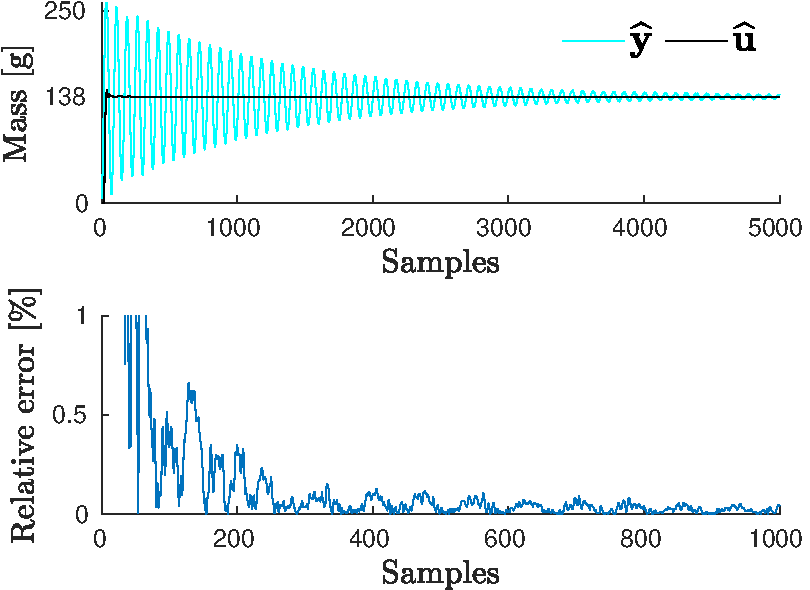
\includegraphics[width=0.69\columnwidth]{./ChapterExperimentalValidation/fig/Fig_1.pdf} 
\caption{ \label{fig:uh_sim} 
Above: example of a simulated response $\widehat{\mathbf{y}}$ and its step input estimation $\widehat{u}$ assuming measurement Gaussian noise with 50 dB of SNR. 
Below: the relative error $|\widehat{u} - u| / u$ is below 1\% after 100 samples. 
We take the estimate at 500 samples because there the relative error is smaller than 0.2\%.  }
\end{figure}

A sensor is a dynamic system, therefore, a fast measurement process must necessarily cope with the system transient response. In that respect we must distinguish between the transient response of the system under test, and the transient phase of the measurement process (i.e. before the process has settled on a final measurement outcome). Notice that the transient phase of the measurement process is considerably smaller than the settling time of the system under test, and this is a major advantage of the step input estimation method.

We are interested in the first element of $\widehat{\bm{\theta}}$, which is the input estimate $\widehat{u}$.
The measurement noise variance was selected to have a signal-to-noise ratio (SNR) in the interval [30 dB, 80 dB], according to \color{blue}(\ref{eqn:SNR})\color{black}. 

The difference between the sample mean $\widehat{\mu}_u$ of the step input estimates and the true value $u$ is the empirical bias $b_\mathrm{e}$.
\begin{equation} {b}_\mathrm{e} = \frac{1}{N_{MC}} \sum_{i=1}^{N_{MC}}{ \widehat{u}_i - u } = \widehat{\mu}_u - u.  \end{equation}

The sample variance $\widehat{\sigma}_u^2$ of the step input estimates is used to obtain the standard error of the MC simulation $\sigma_\mathrm{e}$, which decreases with respect to the square root of the number of MC runs $N_{MC}$. 
\begin{equation}  \sigma_\mathrm{e} = \frac{\widehat{\sigma}_u}{\sqrt{N_{MC}}}, \ \mathrm{where} \ \ \widehat{\sigma}_u^2 = \frac{1}{N_{MC}-1} \sum_{i=1}^{N_{MC}}{ \left( \widehat{u}_i - \widehat{\mu}_u \right)^2 } . \end{equation}

In each of the $N_{MC}$ runs, we compute the predictions of the step input estimation bias and variance from measured data using Equations (\ref{eqn:biasST}) and (\ref{eqn:varST}). 
The step input bias and variance predictions from observed data $b_{\widetilde{\mathrm{p}}}$ and $v_{\widetilde{\mathrm{p}}}$, and the associated standard error $\sigma_{\widetilde{\mathrm{p}}\mathrm{,err}}$, are obtained from
\begin{equation} \begin{aligned} & b_{\widetilde{\mathrm{p}}} = \frac{1}{N_{MC}} \sum_{i=1}^{N_{MC}}{ \mathbf{b}_{\widetilde{\mathrm{p}}}^i \left( \widehat{\bm{\theta}} \right) \big|_{\left[1\right]} }, \ v_{\widetilde{\mathrm{p}}} = \frac{1}{N_{MC}} \sum_{i=1}^{N_{MC}}{ \mathrm{\mathbf{C}}_{\widetilde{\mathrm{p}}}^i \left( \widehat{\bm{\theta}} \right) \big|_{\left[1,1\right]} },  \\ & \mathrm{and} \quad \sigma_{\widetilde{\mathrm{p}}\mathrm{,err}} = \sqrt{   \frac{ \sum_{i=1}^{N_{MC}}{ \left( \mathbf{b}_{\widetilde{\mathrm{p}}}^i \left( \widehat{\bm{\theta}} \right) \big|_{\left[1\right]} - b_{\widetilde{\mathrm{p}}} \right)^2 } }{N_{MC}\left( N_{MC}-1 \right)}  } , \end{aligned} \end{equation}
where $\widetilde{\mathbf{b}}_{\mathrm{p}}^i \left( \widehat{\bm{\theta}} \right) \big|_{\left[1\right]}$ is the first element in the bias vector and $\widetilde{\mathbf{C}}_{\mathrm{p}}^i \left( \widehat{\bm{\theta}} \right) \big|_{\left[1,1\right]}$ is the first element in the covariance matrix obtained in the $i-\mathrm{th}$ approximations.
The predicted bias and variance from exact data are obtained with one evaluation of the expressions
(\ref{eqn:biasE}) and (\ref{eqn:varE})
\begin{equation} b_{\mathrm{p}} = \frac{1}{N_{MC}} \sum_{i=1}^{N_{MC}}{ \mathbf{b}_{\mathrm{p}} \left( \widehat{\bm{\theta}} \right) \big|_{\left[1\right]} }, \ \mathrm{and} \ v_{\mathrm{p}} = \frac{1}{N_{MC}} \sum_{i=1}^{N_{MC}}{ \mathrm{\mathbf{C}}_{\mathrm{p}} \left( \widehat{\bm{\theta}} \right) \big|_{\left[1,1\right]} } . \end{equation}
The uncertainty of the step input estimate is defined as the spread of the estimates that is given by the predicted variance $v_{\mathrm{p}}$.

Figure \ref{bias_sigma_sim_unstr_str_n2} shows the empirical bias, the bias predictions and the standard errors of the MC simulation.
It can be seen that the empirical bias $b_\mathrm{e}$ and the predicted bias $b_{\widetilde{\mathrm{p}}}$ are proportional to the perturbation noise variance while the standard errors $\sigma_\mathrm{e,err}$ and $\sigma_{\widetilde{\mathrm{p}}\mathrm{,err}}$ are proportional to the perturbation noise standard deviation.
For SNR below 40 dB there is a difference of a small order of magnitude between the empirical bias $b_\mathrm{e}$ and the bias prediction $b_{\widetilde{\mathrm{p}}}$. 

The standard errors of the MC simulation $\sigma_\mathrm{e,err}$ and $\sigma_{\widetilde{\mathrm{p}}\mathrm{,err}}$ are smaller than  $b_\mathrm{e}$ and $b_{\widetilde{\mathrm{p}}}$.
The estimates are spread near the sample mean and the uncertainty is smaller than the bias. 
Therefore, the empirical bias of the MC simulation is meaningful.

\begin{figure}[!htb]
\centering
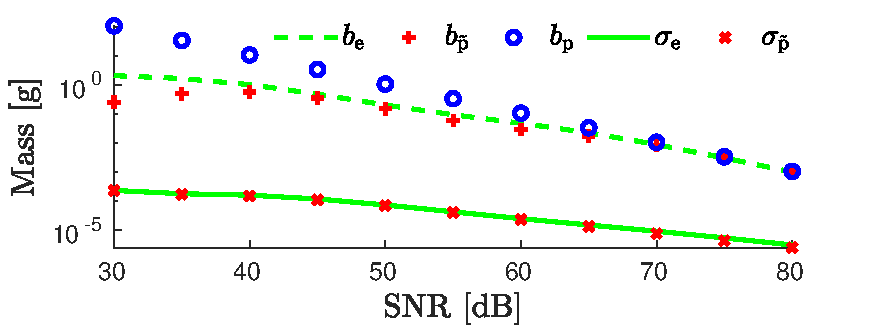
\includegraphics[width=0.69\columnwidth]{./ChapterExperimentalValidation/fig/Fig_2.pdf} 
\caption{ \label{bias_sigma_sim_unstr_str_n2} 
The results of the Monte Carlo simulation of the step input estimation method are the empirical bias $b_{\mathrm{e}}$, the predicted bias using exact data $b_{\mathrm{p}}$, the predicted bias using measured data $b_{\widetilde{\mathrm{p}}}$, the empirical standard error $\sigma_{\mathrm{e,err}}$, and the predicted standard error $\sigma_{\widetilde{\mathrm{p}}\mathrm{,err}}$. The estimation biases are proportional to the perturbation variance and the estimation standard errors are proportional to the perturbation standard deviation. Since the standard errors are smaller than the biases, the MC simulation is meaningful.  }
\end{figure}

The mean squared error (MSE) of the step input estimate, defined as
\begin{equation} \mathrm{MSE} = b^2 + v,   \end{equation}
where $b$ and $v$ are the bias and the variance of the step input estimate, can be applied to the obtained empirical and predicted results and can be compared to the Cram\'er-Rao lower bound (CRLB).
Figure \ref{fig:MSE_CRLB} shows that $\mathrm{MSE}_\mathrm{e} = b_\mathrm{e}^2 + v_\mathrm{e}$ and $\mathrm{MSE}_{\widetilde{\mathrm{p}}}  = b_{\widetilde{\mathrm{p}}}^2 + v_{\widetilde{\mathrm{p}}}$ have the same proportionality with respect to the measurement noise variance as the bound for an unbiased estimator $\mathrm{CRLB_{ub}}$.
For SNR above 35 dB, $\mathrm{MSE}_\mathrm{e}$ and $\mathrm{MSE}_{\widetilde{\mathrm{p}}}$ are equivalent, and below 35 dB the difference between them is of less than a factor of 10.

We obtained an approximation of the $\mathrm{CRLB}_{\mathrm{b}}$ for our biased estimator using the partial derivative of the bias in expression (\ref{eqn:biasST}).
Figure \label{fig:MSE_CRLB} shows that the bounds for the unbiased and biased estimators are almost equal because the partial derivatives of the bias are negligible w.r.t. 1 in Equation (\ref{eqn:CRLB_EIV}).
By adding the square of the predicted bias to the biased estimator bound $\mathrm{CRLB_{b}}$ we obtain an approximation of the minimum MSE that the biased estimator can achieve.
This minimum MSE is close to the CRLBs for large SNR but the square of the bias causes an increase of the MSE around 35 dB.
The differences between the CRLBs and $\mathrm{MSE}_\mathrm{e}$ and $\mathrm{MSE}_{\widetilde{\mathrm{p}}}$ are of one order of magnitude for large SNR and become small for SNR lower than 40 dB.
This difference is the cost of solving a structured EIV problem with a simple LS method.
%Therefore, for large measurement noise variance, the step input estimation method produces results that are comparable to maximum-likelihood estimation, since $\mathrm{MSE}_{\widetilde{\mathrm{p}}} \approx \mathrm{CRLB_{b}} + b_{\widetilde{\mathrm{p}}}^2$.


\begin{figure}[!htb]
\centering
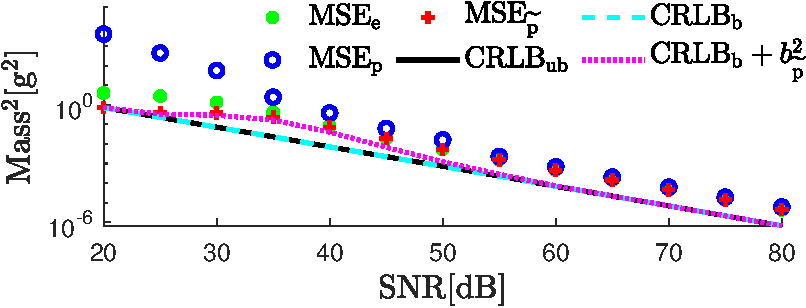
\includegraphics[width=0.69\columnwidth]{./ChapterExperimentalValidation/fig/Fig_3.pdf}
\caption{\label{fig:MSE_CRLB} The observation instant is fixed at 500 samples.
The bias and the MSEs decrease for large SNR. 
The empirical $\mathrm{MSE_e}$ and the predicted $\mathrm{MSE}_{\widetilde{\mathrm{p}}}$ of the step input estimation are one order of magnitude larger than the Cram\'er-Rao lower bound.
Adding the CRLB for a biased estimator with the predicted bias squared we have the minimum MSE, that grows in the interval [25 dB, 45 dB].
Below 35 dB the difference between $\mathrm{MSE}_{\widetilde{\mathrm{p}}}$ and the CRLB is less than a factor of 10.}
\end{figure}

There are two features of the system step response that make the CRLB small.
One is the measurement noise variance and the second is sample size.
The estimation from step response perturbed with small noise variance has lower uncertainty.
Also, using larger sample size to perform the estimation boils down to smaller estimation uncertainty.

In order to get more insight into the step input estimation method we conducted another simulation study. 
The step input estimation method assumes the order $n$ is given in (\ref{eqn:min_seiv}).
In this simulation, the step input estimation method processed the step response generated by a $5-th$ order system using different values of $n$ in the interval from 2 to 100.

The step response is perturbed with Gaussian white noise with SNR values in the interval [20 dB, 80 dB].
For each order $n$ and SNR value, 100 step input estimations are performed from independent noise realizations. 
Figure \ref{fig:msee_vs_n_sim} shows the average of the squared biases and the variances, and the MSEs of the input estimate using the first 500 samples.
It is evident that the estimation variance and MSE depend on the SNR.

Increasing the order $n$ is equivalent to adding more regressors in the regression problem.
It is well known that increasing the order $n$ causes a monotonic decrement of the estimation bias and increment of the variance.
This is the asymptotic behavior of the estimation statistical moments with respect to the number of regressors.
Nevertheless, the simulation results presented in Figure \ref{fig:msee_vs_n_sim} show that the variance first increases for small values of $n$, followed by a decrement and finally after $n \approx 40$ the variances exhibit a slow and steady increment. 
This apparent contradiction does not prove the invalidity of the estimation method since the results presented correspond to a finite sample size and the asymptotic results cannot be applied.
The theoretical explanation of the estimation statistics for finite sample sizes is out of the scope of this document.

 
There is a bias-variance tradeoff and the MSEs exhibit local minima with respect to $n$.
The principal contribution to the MSE is the squared bias for the smaller values of $n$ and the variance for the larger values of $n$. 
However, the higher orders do not produce overfitting since the MSEs do not grow fast and remain close to the minimum values. 

The optimum value of $n$ is not necessarily equal to the order of the generating system and varies for each SNR.
According to the plots in Figure \ref{fig:msee_vs_n_sim}, there are orders that provide local minima of the step input estimation MSEs.
From the right hand side of Figure \ref{fig:msee_vs_n_sim}, the orders that give the first two MSE minima were identified and those values are listed in Table \ref{Tbl:orders}.
For each SNR, there is a first minimum at a low order and a second minimum at a high order.
For SNR of 30 and 40 dB, it is recommended to use the order that gives the first minimum since the MSE at the second minimum is less than one order of magnitude smaller than at the first minimum.
Depending on the requirements, the user can choose between the simplicity of an estimation with a low order or an estimation with higher computational complexity and a smaller MSE. 
In a calibration stage, during the setup of the estimation method, the user can search and set the order that enables the estimation method to provide a required MSE.



\begin{table}[!ht]
\caption{ Orders $n$ that provide local minima for the MSE of the step input estimate. It is recommended to use the order that gives the first minimum when there is a difference of small order of magnitude with respect to the MSE at the second minimum.} 
\label{Tbl:orders} 
\centering
\begin{tabular}{c|c c c c} 
\hline
SNR [dB] & 30 & 40 & 50 & 60 \\
\hline
order at first minimum & 11 & 7 & 4 & 3 \\ 
order at second minimum & 40 & 35 & 40 & 31 \\
\hline
\end{tabular}
\end{table}

\begin{figure}[!htbp]
\centering
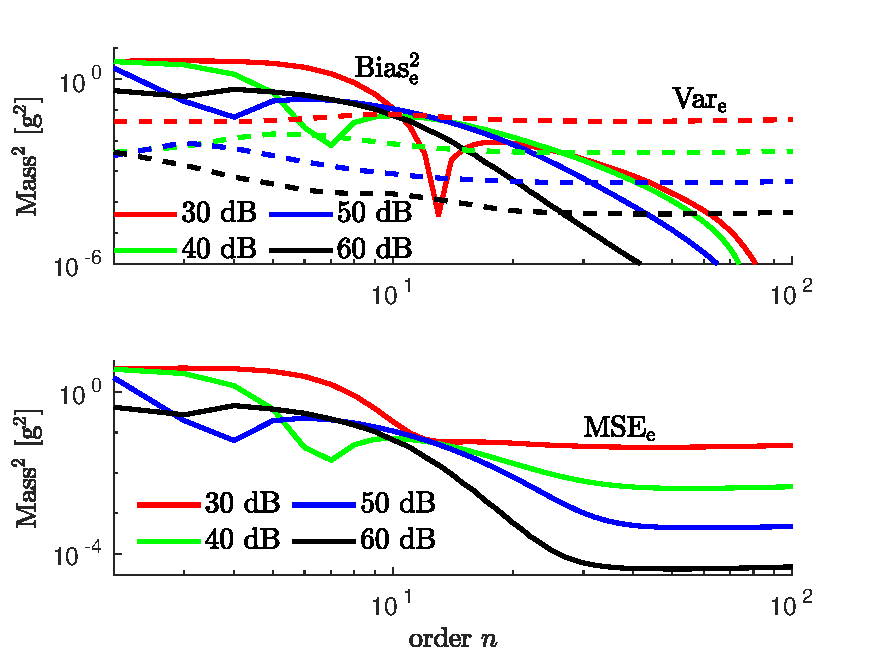
\includegraphics[width=0.69\columnwidth]{./ChapterExperimentalValidation/fig/Fig_4.pdf} 
\caption{ \label{fig:msee_vs_n_sim} 
The simulated step responses of a $\mathrm{5-}th$ order system are processed by the step input estimation method using different orders $n$ and independent noise realizations. 
The perturbation of the step responses is Gaussian white noise with SNRs of 30, 40, 50, and 60 dB.
The square of the empirical bias (solid) and the empirical variance (dashed) are shown on the left hand side and the MSE is shown on the right hand side, for $n$ between 2 and 100.
These results suggest that, during the setup of the estimation method, we have to search the order that gives the minimum MSE without increasing unnecessarily the complexity of the estimation method.  }
\end{figure}


% \begin{figure}
% \centering
% \includegraphics[width=0.5\columnwidth]{./msee_vs_n_sim.pdf} 

%\end{figure}


\section{Practical implementation} 
An experimental setup was constructed to test the step input estimation method.
The implementation is a weighing system that uses a load cell Tedea Huntleigh 1004, whose specifications are found in  \citet{tedea1004}.
The maximum rating of the load cell is 600 g.
A cylindrical aluminium object of 138.32 g of mass was used to excite the load cell.
This value was found by calibration using a balance KERN PCB 200-2 that has an uncertainty of 0.01 g.
The step input excitation was provided by a magnet that holds and releases a mass from above the load cell.
The magnet is located sufficiently far from the load cell to avoid magnetic interference in the sensor response.

\ctikzset{bipoles/resistor/height=0.075}
\ctikzset{bipoles/resistor/width=0.25}
\begin{figure}[!htb]
\centering
\begin{tikzpicture}[every node/.style={draw,outer sep=0pt,thick}]
\tikzstyle{spring}=[thick,decorate,decoration={zigzag,pre length=0.3cm,post length=0.3cm,segment length=6}]
\tikzstyle{damper}=[thick,decoration={markings,  
  mark connection node=dmp,
  mark=at position 0.5 with 
  {
    \node (dmp) [thick,inner sep=0pt,transform shape,rotate=-90,minimum width=15pt,minimum height=3pt,draw=none] {};
    \draw [thick] ($(dmp.north east)+(2pt,0)$) -- (dmp.south east) -- (dmp.south west) -- ($(dmp.north west)+(2pt,0)$);
    \draw [thick] ($(dmp.north)+(0,-5pt)$) -- ($(dmp.north)+(0,5pt)$);
  }
}, decorate]
\tikzstyle{ground}=[fill,pattern=north east lines,draw=none,minimum width=0.63cm,minimum height=0.3cm]

% load cell
\node (M1) [minimum width=1.6cm,minimum height=0.4cm, xshift=-3cm, yshift=-1cm] {};

\node (ground1) at (M1.east) [ground,yshift=0.0cm,rotate=90,xshift=0.0cm,anchor=north] {};
\draw (ground1.north east) -- (ground1.north west);

\node at (M1.north) [fill=none, xshift=-0.75cm, yshift=0.750cm] (2.0cm, 1.50cm) {\small Mass};
\draw (M1.north) [-latex,thick]  ++(-0.75cm,0.5cm) -- +(0cm,-0.5cm);
\draw (-3.3750cm,-0.935cm) arc(30:330:1.25mm);
\draw (-2.625cm,-1.05cm) arc(210:510:1.25mm);
\draw (M1.west) [thick]  ++(0.4cm, 0.0750cm) -- +(0.80cm,0.0cm);
\draw (M1.west) [thick]  ++(0.4cm,-0.0750cm) -- +(0.80cm,0.0cm);

\node at (M1.south) [align=center, draw=none,fill=none, xshift=0.0cm, yshift=-0.5cm] (2.0cm, 1.50cm) {\small load cell \\ \small Tedea 1004};

% amplifier
\draw (-1.6,-0.0) -- (-1.6,-2.0) -- (1.2,-1) -- cycle;
    \draw (-1.5,-1) to[R] (-1.1,-0.6) to[R] (-0.7,-1);
    \draw (-1.5,-1) to[R] (-1.1,-1.4) to[R] (-0.7,-1);
\draw [-latex,thick]  ++(1.2,-1) -- +(0.8,0);

\node (filter) [minimum width=0.50cm,minimum height=0.50cm, xshift=-0.0cm, yshift=-1cm] {};
\draw [thick]  ++(-0.275,-0.9) -- +(0.275,0.0);
\draw [thick]  ++(0,-0.9) -- +(0.25,-0.250);
\node at (M1.east) [draw=none, fill=none, xshift=4.0cm, yshift=0.25cm] (2.0cm, 1.50cm) {$\widetilde{y}$};
% wire
\draw plot [smooth] coordinates {(-2.3,-0.8) (-2.2,-0.5) (-1.7,-0.5) (-1.65,-0.9) (-1.6,-1)};

\node at (M1.south) [align=center, draw=none,fill=none, xshift=3.75cm, yshift=-0.750cm] (2.0cm, 1.50cm) {\small amplifier and filter};

\node (ADC) [align=center, minimum width=1.2cm,minimum height=0.9cm, xshift=2.6cm, yshift=-1cm] {\small ADC \\ \small 16 bits};

\end{tikzpicture}
\caption{Diagram of the load cell and the conditioning amplifier that provide the sensor response.} \label{lcm}
\end{figure}

A two-stage linear conditioning amplifier performs amplification and filtering of the load cell signal.
The first stage is a precision instrumentation amplifier INA114 that has high common mode rejection ratio.
The second stage is a third-order low-pass Butterworth filter with cut-off frequency of 100 Hz.
The low-pass filter prevents the aliasing noise in the measured transient response.
The signal obtained from the conditioning amplifier is considered to be the response of the sensor.
The sensor responses to step excitations were sampled with a frequency of $f_s=4$ kHz, and therefore the Nyquist frequency is 2 kHz.
The step responses were collected and stored as datasets for further analysis.
\color{blue}The datasets, and the code used to generate the results in this section \href{https://drive.google.com/drive/folders/1EfQb4nccg6x4kGcZropKRug3WkeNGX-m?usp=sharing}{\color{blue}are publicly available} in the sense of reproducible research research in the following url: \href{https://drive.google.com/drive/folders/1EfQb4nccg6x4kGcZropKRug3WkeNGX-m?usp=sharing}{https://drive.google.com/drive/folders/1EfQb4nccg6x4kGcZropKRug3WkeNGX-m?usp=sharing}\color{black}.  
The number of samples collected for each step response is $N=20000$.
For practical purposes, we consider that the last 10000 samples correspond to the steady state response.
%The datasets are available in the following repository: %[[https://www.dropbox.com/sh/0dlam0rqqiynyiq/AAAq0H9rFxpkQON4zkmPXPXXa?dl=0][dropbox folder]]. 
\begin{figure}[!htb]
\centering
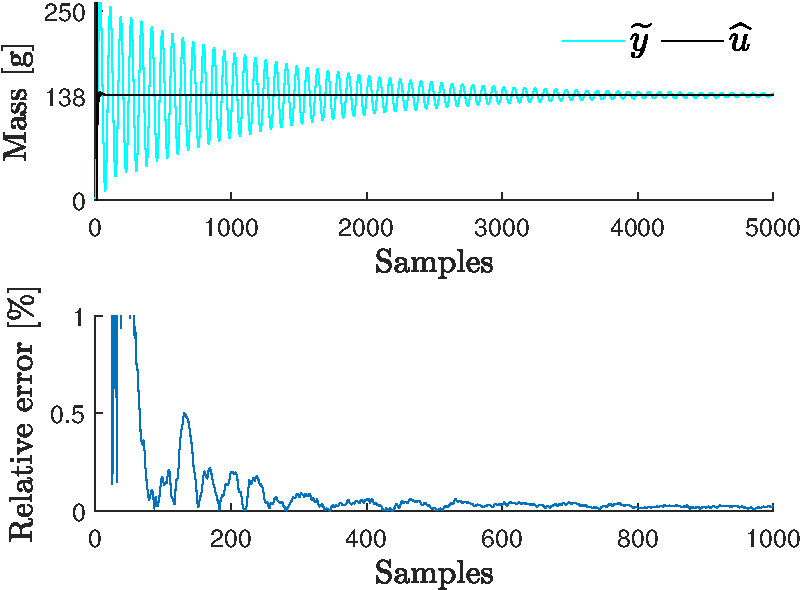
\includegraphics[width=0.69\columnwidth]{./ChapterExperimentalValidation/fig/Fig_6.pdf} 
\caption{ \label{fig:uh_exp} 
Above: a typical measured sensor transient response $\widetilde{y}$ takes more than 1.25 s (5000 samples, $f_s = 4$ kHz) to converge to the steady state response. 
Below: the relative error of the input estimate $\widehat{u}$ is smaller than 0.2\% from 300 samples.
We consider that at $500$ samples the relative error of the estimate $\widehat{u}$ is small enough to consider that $\widehat{u}$ is close to its expected value $u$.  }
\end{figure}

The step input estimation method processed 100 measured sensor step responses, assuming the sensor is of $\mathrm{7-}th$ order.
Figure \ref{fig:uh_exp} shows a typical measured transient response $\widetilde{y}$ and an example of the estimated input $\widehat{u}$.

The empirical bias $b_{\mathrm{e}}$ is the difference between the average of the 100 estimates $\widehat{u}$ and the mass calibration value $u = 138.32$ g, at each instant of time, and the standard error $\sigma_\mathrm{e,err}$ is the standard deviation of the mean estimate of the responses processed, i.e.,
\begin{equation} \begin{aligned} \widehat{\mu}_{\mathrm{e}} &= \frac{1}{100} \sum_{i=1}^{100}{ \widehat{u}_{i} }, \quad {b}_{\mathrm{e}} = \widehat{\mu}_{\mathrm{e}} - u, \quad \mathrm{and} \\  \sigma_{\mathrm{e,err}} &= \frac{\widehat{\sigma_\mathrm{e}}}{\sqrt{100}}, \quad \mathrm{where} \ \widehat{\sigma_\mathrm{e}}^2 = \frac{1}{99} \sum_{i=1}^{100}{ \left( \widehat{u}_i - \widehat{\mu}_{\mathrm{e}} \right)^2 } . \end{aligned} \end{equation}


The bias $\widetilde{b}_{\mathrm{p}}$ and variance $\widetilde{v}_{\mathrm{p}}$ predictions from the measured data were obtained by processing off-line the 100 measured sensor transient step responses with expressions (\ref{eqn:biasST}) and (\ref{eqn:varST}).
These expressions require the measurement noise variance $\sigma_\epsilon^2$ to obtain the bias and variance prediction.
One way to estimate the measurement noise variance is computing the variance of each sensor steady state response, see Figure \ref{fig:y_ss}.
Later in this section we will explore another way to estimate the measurement noise variance.
Computing the noise variance from the steady state response we observed that the SNR of the measured step responses is 55 dB in average.

\begin{figure}[!htb]
\centering
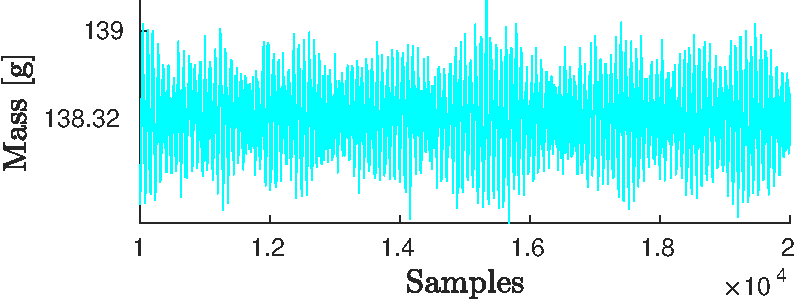
\includegraphics[width=0.69\columnwidth]{./ChapterExperimentalValidation/fig/Fig_7.pdf}
\caption{ \label{fig:y_ss} 
From the sensor steady-state response an estimation of the measurement noise variance is obtained.}
\end{figure}

Figure \ref{fig:b_sigma_exp_str} shows the empirical bias $b_{\mathrm{e}}$ and the standard error $\sigma_{\mathrm{e,err}}$ that result after processing the first $\color{blue}N\color{black}=500$ samples of the 100 measured step responses $\widetilde{\mathbf{y}}$.
The standard error is smaller than the bias.
As it was observed in the MC simulation, this is the uncertainty of the estimation method.
The oscillations observed in the bias are mainly due to the transient response and not to the measurement noise.
The measurement noise effects are partially removed since we averaged the 100 transient responses, 
which is a small number compared with the $N_{MC}$ runs averaged in the simulation section. 

It is expected that the empirical bias is large when a small number of samples is processed. 
The data-driven input estimation method is recursive and it is implemented in real-time.
The estimation errors decrease as more data is processed.

\begin{figure}[!htb]
\centering
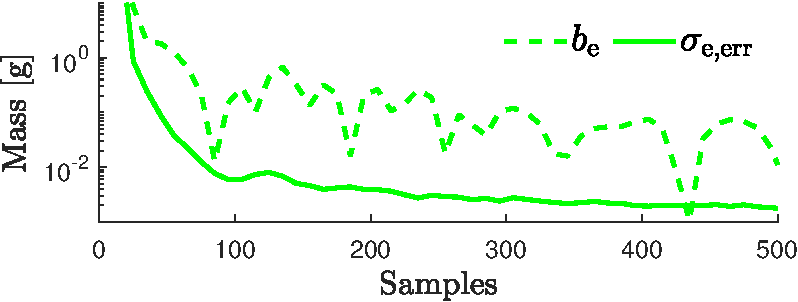
\includegraphics[width=0.69\columnwidth]{./ChapterExperimentalValidation/fig/Fig_8.pdf} 
\caption{ \label{fig:b_sigma_exp_str} 
The results of estimating the step input level after processing 100 measured step responses are the empirical bias $b_{\mathrm{e}}$ and the empirical standard error $\sigma_{\mathrm{e,err}}$. 
The estimation bias and the estimation standard error decrease as more samples are processed. 
The estimation bias is affected by the transient effects of the sensor response.  
The values of $b_{\mathrm{e}}$ and $\sigma_{\mathrm{e}}$ provide the estimate accuracy and uncertainty for a given sample size.
}
\end{figure}

The measurement noise is not white since there is evidence of frequency components in the sensor steady state response that are observed as oscillations in Fig \ref{fig:y_ss}.
To get insight into the properties of the measured sensor response $\widetilde{\mathbf{y}}$, a $\mathrm{7-}th$ order model was identified from input-output data assuming that the input is a step of level $u$.
A response $\widehat{\mathbf{y}}$ was simulated from the identified model and the residual $\mathbf{r} = \widetilde{\mathbf{y}} - \widehat{\mathbf{y}}$ was obtained. 
We can observe these signals in the frequency domain using the discrete Fourier transform, that for the signal $\widetilde{\mathbf{y}}$ is defined as 
\begin{equation} \widetilde{Y}(f) = \dfrac{1}{\sqrt{N}} \sum_{k=0}^{N-1} \widetilde{y} \left( k \right) e^{-j2\pi k f / N} \label{eqn:FFT} \end{equation}
where $f = 1, \ldots, N/2$ are the frequency lines and $N$ is the total number of samples.
The power spectrum of the signal $\widetilde{\mathbf{y}}$ is given in decibels by $\widetilde{\mathbf{Y}}_\mathrm{dB} = 20 \log_{10}{ |\widetilde{\mathbf{Y}}| } $.
Figure \ref{fig:YYhR_n7} shows the corresponding power spectra of the sensor response $\widetilde{\mathbf{Y}}_\mathrm{dB}$, the simulated response $\widehat{\mathbf{Y}}_\mathrm{dB}$, and the residual $\mathbf{R}_\mathrm{dB}$. 
There are frequency components near the main resonance peak in the magnitude spectrum of the residual.
The presence of frequency components near the main resonance peak is commonly found in mechanical devices.
The vibrations captured from the environment explain the accumulation of energy near the main resonance modes.

\begin{figure}[!htb]
\centering
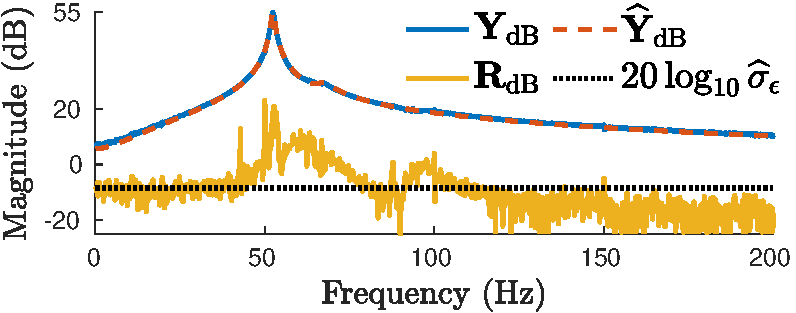
\includegraphics[width=0.69\columnwidth]{./ChapterExperimentalValidation/fig/Fig_9.pdf}
\caption{ \label{fig:YYhR_n7} 
The power spectra of a measured response $\widetilde{\mathbf{Y}}_\mathrm{dB}$, a simulated response $\widehat{\mathbf{Y}}_\mathrm{dB}$, and the residual $\mathbf{R}_\mathrm{dB}$ is not flat and then the measurement noise is not white. 
The average of the residual power spectrum provides a conservative estimate of the measurement noise variance $\widehat{\sigma}_\epsilon^2$, represented with the dotted line.}
\end{figure}

Even when the residual $\mathbf{r}$ is not white, it provides an alternative way to estimate the measurement noise variance. 
The average of the residual power spectrum approximates the measurement noise variance as follows
\begin{equation} \widehat{\sigma}_\epsilon^2 \approx \dfrac{2}{N} \sum_{f = 1}^{N/2} \left| R \left( f \right) \right|^2 . \label{eqn:P_R} \end{equation}
The dotted line in Figure \ref{fig:YYhR_n7} indicates the $10 \log_{10} \left( \widehat{\sigma}_\epsilon^2 \right)$ level of the measurement noise variance estimated from the residual.
This level is higher than the mean value of the residual power spectrum $\mathbf{R}_\mathrm{dB}$ in the frequencies above 120 Hz.

Using the residual power spectra that correspond to the measured step responses, we obtained the measurement noise variance and the SNR for each experiment.
Figure \ref{fig:meas_SNR} shows the estimated SNRs from the residual power spectra. 
The SNR mean value is 50 dB.
Therefore, we assume that the SNR of the measured transient responses is 50 dB instead of 55 dB, as it was estimated from the steady state response.

\begin{figure}[!htb]
\centering
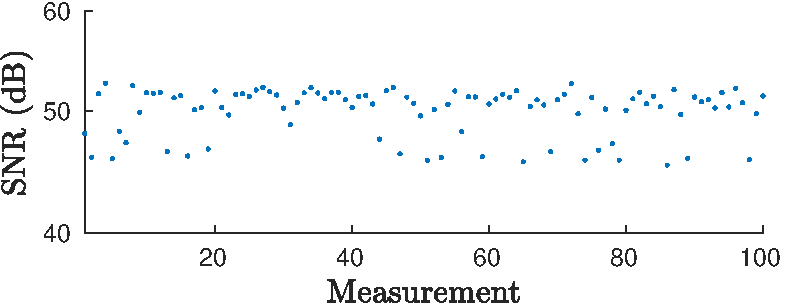
\includegraphics[width=0.69\columnwidth]{./ChapterExperimentalValidation/fig/Fig_10.pdf}
\caption{ \label{fig:meas_SNR} 
The mean value of the signal-to-noise ratios estimated from the residual power spectra is 50 dB.
We consider that this is the estimated SNR of the measured step responses.}
\end{figure}

The 5 dB difference provides a conservative bound since the bias and variance computed from 50 dB of SNR are higher than those obtained using the variance estimation from the steady-state response. 
Figure \ref{fig:b_sigma_exp_str2} shows a comparison of the results obtained with both measurement noise variance estimations after processing the first $\color{blue}N\color{black}=500$ samples of the step response $\widetilde{\mathbf{y}}$.
Using expression (\ref{eqn:biasST}), the bias prediction  $b_{\widetilde{\mathrm{p}}2}$ obtained using an SNR of 50 dB approximates more closely the empirical bias than $b_{\widetilde{\mathrm{p}}1}$ obtained using an SNR of 55dB.
In accordance, the standard error of the bias predictions $\sigma_{\widetilde{\mathrm{p}}\mathrm{,err2}}$ is larger than $\sigma_{\widetilde{\mathrm{p}}\mathrm{,err1}}$ and is a conservative measure of the input estimation uncertainty.
In conclusion, using the noise variance estimated from the residual prevents underestimating the step input estimation uncertainty.


\begin{figure}[!htb]
\centering
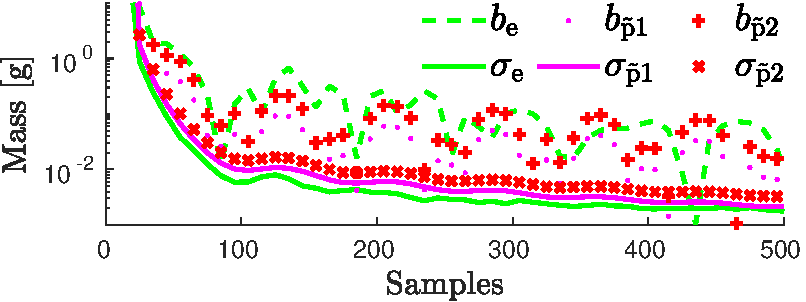
\includegraphics[width=0.69\columnwidth]{./ChapterExperimentalValidation/fig/Fig_11.pdf} 
\caption{ \label{fig:b_sigma_exp_str2} 
Comparative view of the bias prediction using two different noise variance estimations. 
Estimating the variance from the step response residual gives a bias prediction $b_{\widetilde{\mathrm{p}}2}$ and a standard error $\sigma_{\widetilde{\mathrm{p}}\mathrm{,err2}}$ that are slightly higher than $b_{\widetilde{\mathrm{p}}1}$ and $\sigma_{\widetilde{\mathrm{p}}\mathrm{,err1}}$ which correspond to computations that use the noise variance estimated from the steady state response. 
The bias prediction $b_{\widetilde{\mathrm{p}}2}$ approximates better the empirical bias. 
The standard error $\sigma_{\widetilde{\mathrm{p}}\mathrm{,err2}}$ provides a conservative value of the input estimation uncertainty. }
\end{figure}


We investigated another aspect of the step input estimation method performance when processing measured step responses.
The step input estimation method requires an assumption of the generating system order in the formulation of the estimation problem (\ref{eqn:min_seiv}).
The estimation method performance is assessed under different assumptions of the values of $n$ in the interval from 2 to 100. 
For each value of $n$, 100 step input estimations are computed from measured transient responses and the empirical MSEs are compared.
Figure \ref{fig:msee_vs_n_exp} shows that, similar to the observations made in the simulation study, the MSEs have two local minima at $n=7$ and $n=48$.
It is recommended to use $n = 7$ in the estimation method to provide a small estimation MSE without the higher computational complexity that $n=48$ implies.


\begin{figure}[!htbp]
\centering
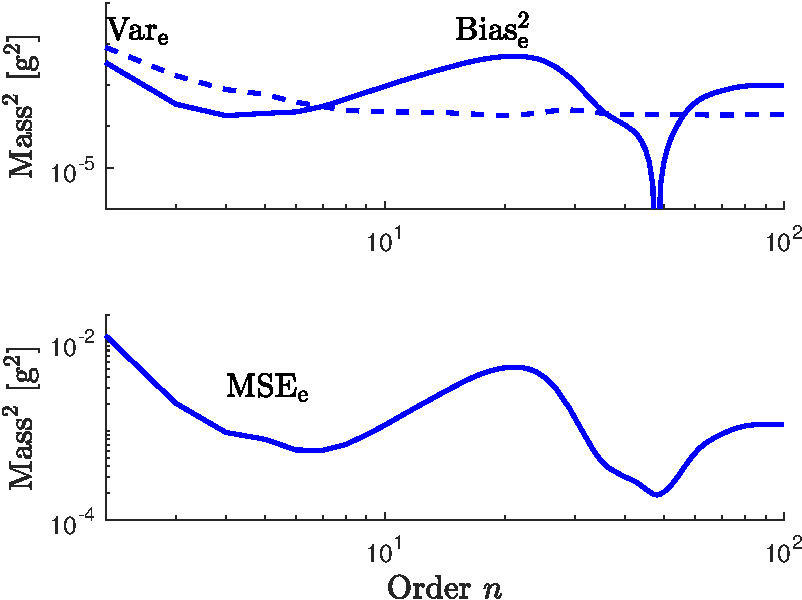
\includegraphics[width=0.69\columnwidth]{./ChapterExperimentalValidation/fig/Fig_12.pdf} 
\caption{ \label{fig:msee_vs_n_exp} 
The hundred measured sensor step responses are processed by the step input estimation method for different values of the order $n$. 
The empirical squared bias (solid) and the empirical variance (dashed) are shown on the left and the empirical MSE on the right.
The MSE has a local minimum at $n=7$ and another at $n=48$.
It is recommended to use the estimation method with $n=7$ because at $n=48$ the decrement of the MSE is not significant.  }
\end{figure}

\section{Conclusions}

In this chapter we investigated the statistical properties of a data-driven step input estimation method in a real-life application.
The step input estimation method is a structured and correlated errors-in-variables problem that is solved with recursive least-squares.
A statistical analysis was conducted using the ordinary least-squares condensed notation. 
This statistical analysis of the input estimate provides expressions that approximate the estimation bias and variance assuming that the measurement noise is Gaussian white noise. 
The variance approximation is useful to assess the uncertainty of the input estimate.
In simulation we observed that the mean squared error of the input estimate is close to the theoretical minimum that uses the Cram\'er-Rao lower bound for biased estimators.
Since the data-driven step input estimation method is not statistically efficient, there is room for improvement. This is a topic for future research.
In the practical experiments, the measurement noise is not white.
The noise variance obtained from the sensor steady state response underestimates the measurement noise variance, that was observed 5 dB larger in the power spectrum due to nonlinearities of the sensor.
Considering this difference in the measurement noise variance, we introduced a conservative bound of the measurement noise variance so that the first and second moments of the input estimate are more accurately predicted.
Using the variance approximation, we can assess the uncertainty of the input estimate with respect to the number of samples processed by the data-driven step input estimation method.
The step input estimation method is useful in practical applications where the whiteness assumption of the measurement noise is not fulfilled. 


%\newpage



\glsresetall

\chapter{Ramp input estimation method}\label{chap:RampInput}

\begin{quote}
\emph{The results of this chapter ...}\vfill{}
\end{quote}


\section{Introduction}

The goal of a measurement is to accurately estimate the input value using the sensor transient response.
The input might vary during the measurement being the simplest case the input that changes with a constant rate, described with an affine function.
The inputs that vary at a constant rate activate the sensor gradually. 
An affine input estimation method is needed to estimate the slope and the interception parameters of the affine function.

This chapter describes two signal processing methods for the estimation of affine input parameters.
These methods are a data-driven subspace method and a maximum-likelihood (ML) estimation method based on local-optimization.
The subspace is a recursive method independent of the sensor model, and the ML method iteratively minimizes a cost function using a simulated sensor response in a receding time horizon.

In this chapter, the dynamic weighing is chosen as an implementation example.
The dynamic weighing of an affine input is an interesting metrology application because the affine input turns a linear time invariant sensor model into a time-varying sensor model.
The affine input estimation methods provide an insight on the properties of the dynamic measurement of time-varying inputs.

The effectiveness and the uncertainty of the methods are evaluated with simulation studies.
The uncertainty is assessed, for the subspace method, using a Taylor expansion of the exponentially weighted recursive least squares estimate, and
for the ML method, using the derivatives of the residual error obtained from the to-be-minimized cost function.

\begin{comment}
Measurements estimate the unknown value of a physical quantity, namely the measurand.
The to-be-measured physical quantity is applied as an input signal to a sensor. 
The sensor is a dynamical system and its output changes as a consequence of the input excitation and the sensor initial conditions.
The goal of a measurement is to estimate accurately the measurand value using the sensor transient response.
The transient response of a stable sensor decays to a steady state response.
In steady state, the most accurate estimation of the input true value is simply found using the sensor static gain.
However, the steady state is reached in theory after an infinite period of time and in practice we require fast estimations.
The trade-off between accuracy and speed exists in all measurements.

The measurand can be assumed to be constant or variable during the measurement.
A dynamic measurement is present when the fluctuations of the measurand impact on the input estimation.
A typical example of a dynamic measurement problem is a low-bandwidth sensor excited with a fast changing input.
Some characteristics of the input, like the minimum or maximum or the effects of the environment on the measured quantity, occur in small periods of time.  
The detection of the input characteristics is needed in several scientific and industrial applications such as measurements of temperature \cite{Saggin01}, pressure \cite{Matthews14}, acceleration \cite{Link07}, force \cite{Vlajic16, Hessling08a} and mass \cite{Shu93, Boschetti13}.

The solution to dynamic measurement problems is non-trivial.
An approach is to add a dynamical system to compensate the sensor transient response, inverting the effects of the sensor dynamics.
The purpose of such a compensator is to reduce the transient time.
The sensor dynamics are considered in the design of finite and infinite impulse response compensation digital filters based on deconvolution \cite{Eichstadt10} or synthesized to correct dynamic errors \cite{Hessling08a}. 
The model-based deconvolution design of compensators implies that the measurand true value should be known a-priori for certain applications, such as mass determinations \cite{Boschetti13, Niedzwiecki16b}.
In the literature most of the measurements systems are assumed linear time-invariant, but the compensation digital filters can be linear \cite{Tasaki07},  nonlinear \cite{Shu93} or time-varying \cite{Pietrzak14}.

The digital signal processors enable a different approach where the input estimation can be obtained with algorithms that do not necessarily recreate the dynamics of a system.
One of the authors of this paper proposed a data-driven signal processing method that estimates the measurand true value using subspace techniques \cite{Markovsky15cep, Markovsky15ieee}.
The subspace estimation method bypasses the model identification step to estimate the unknown input directly from the response data.
This method was developed to estimate inputs modeled as step functions of unknown scaling level.
We extended the subspace input estimation method to estimate the parameters of inputs that vary at a constant rate.

The inputs that vary at a constant rate are found in applications where the measurand activates the sensor gradually. 
An example of this activation is the measurement of mass while the to-be-weighted object is transported by a conveyor belt, and the profile of the input is a saturated ramp.
Current solutions to the weighing in motion are low pass filters that estimate the mass using the saturated ramp \cite{Tasaki07, Pietrzak14}.
The signal processing affine input estimation methods are motivated by the need to obtain the mass of the object from the ramp before it reaches saturation.
The ramp is parameterized as a straight line model where the slope and the interception are the parameters of interest.

This paper describes a subspace method for the estimation of the affine input parameters.
This method is a recursive algorithm that can be implemented in real-time since it has low computational cost.
The subspace method is independent of the sensor model and, therefore, it is suitable for a variety of applications.
The dynamic weighing is one of the applications and was chosen as an implementation example.
The effectiveness of the method is evaluated in a simulation study.
The performance of the proposed method is compared to that of a maximum-likelihood (ML) estimation method based on local-optimization and a time-varying compensation filter.
%We found that the subspace method obtains the slope estimate from the sensor transient response using the same assumptions of the data-driven step input estimation method.

The ML method resembles the model predictive control approach in the sense that a cost function is minimized iteratively to optimize the parameters of a sensor model using the observed sensor response in a receding time horizon \cite{Mayne14}.
The difference is that the ML method aims to estimate the unknown value of the affine input parameters instead of identifying a model and controlling the dynamic system.
The ML method is more appropriate for off-line processing of the sensor transient response.
Nevertheless, the ML method can estimate the parameters of the affine input, the parameters of a sensor model, and the initial conditions of the sensor.

The uncertainty of the subspace method is assessed using a Taylor expansion of the estimate and Monte Carlo random sampling approach \cite{Quintana19}.
The Monte Carlo approach requires a large set of generated random samples, and for simple systems it is the recommended method.
There exists a deterministic sampling approach to study the uncertainty propagation of complex systems \cite{Hessling13a, Hessling13b}. 
Deterministic sampling aims to represent the minimal statistical information that is relevant to the uncertainty estimation in a finite set.
The uncertainty of the ML method is assessed using the derivatives of the residual error that constructs the to-be-minimized cost function.
The covariance of the optimization method estimate is found using the inverse of the Hessian matrix \cite{Pintelon12Book}.

\end{comment}




\subsection{Affine input estimation problem}

The affine input is modeled as a straight line $u = {a} t + {b}$ with parameters the slope $a$ and the interception $b$.
The affine input estimation problem is formulated as a signal processing problem as follows. 


\paragraph{Problem} 
Given the sequence of measured output observations $\mathbf{y} = \left( y(1),\ldots,y(T)\right), y(t) \in {\rm I\!R}$, of a stable linear time-invariant system of order $n$, and static gain $\gamma$, generated by an affine input $u = \widebar{a} t + \widebar{b}$, estimate the parameters of the affine input, \textit{i.e.,} find the values of the parameters $\widehat{a}, \widehat{b} \in {\rm I\!R}$ such that $\widehat{u} = \widehat{a} t + \widehat{b}$ approximates $u$.
The measured observations $\mathbf{y} = \widebar{\mathbf{y}} + \bm{\epsilon}$ are exact sensor responses $\widebar{\mathbf{y}}$ perturbed by additive noise  $\bm{\epsilon}$ assumed to be independent and normally distributed of zero mean and given variance $\sigma_{\epsilon}^2$.

\paragraph{Motivating example}
Dynamic weighing is an application example where the affine input can be observed.
The weighing of objects in a conveyor belt gives the sensor input an ideal straight line profile when the conveyor belt moves at a constant speed.
The straight line represents the mass coming gradually into the weighing scale sensor in the conveyor belt.
The mass can be estimated from the slope $a$ of the straight line model. 
The mechanical vibrations of the conveyor belt perturb the input and the sensor response is affected by measurement noise.
The interest is to estimate the mass of the object using the sensor response observations.

Consider the weighing scale modeled as a second order mass-spring-damper system, such as the one shown in the diagram of Figure \ref{fig:msd_system}.
The application of an affine input turns the linear time-invariant system into a linear time-varying system, whose
dynamics depends on the input $u(t) = \widebar{a} t + \widebar{b}$, as it is described by the differential equation:
\begin{equation} \dfrac{d}{dt} \left( \left( \widebar{a} t + \widebar{b} + m \right) \dfrac{dy}{dt} \right) + k_{\mathrm{d}} \dfrac{dy}{dt} + k_{\mathrm{s}} y = \left( \widebar{a} t + \widebar{b} + m \right) g \end{equation}
where $m$ is the mass of the scale, $k_{\mathrm{d}}$ is the damping constant, $k_{\mathrm{s}}$ is the elasticity constant, and $g = 9.81$ $\mathrm{m/s}^2$ is the gravitational acceleration. 

The weighing system admits a state space representation where the states $x_1=y$ and $x_2=\dot{y}$ are the position and the speed of the weighing scale: 
\[ \dot{\mathbf{x}} = \begin{bmatrix} 0 & 1 \\ \dfrac{-k_{\mathrm{s}}}{\widebar{a} t + \widebar{b} + m} & \dfrac{-(k_{\mathrm{d}} + \widebar{a})}{\widebar{a} t + \widebar{b} + m} \end{bmatrix} \mathbf{x} + \begin{bmatrix} 0 \\ g \end{bmatrix},  \quad y = \begin{bmatrix} 1 & 0  \end{bmatrix} \mathbf{x} . \]


\begin{figure}[htb!]
\centering

\begin{tikzpicture}[every node/.style={draw,outer sep=0pt,thick}]
\tikzstyle{spring}=[thick,decorate,decoration={zigzag,pre length=0.3cm,post length=0.3cm,segment length=6}]
\tikzstyle{damper}=[thick,decoration={markings,  
  mark connection node=dmp,
  mark=at position 0.5 with 
  {
    \node (dmp) [thick,inner sep=0pt,transform shape,rotate=-90,minimum width=15pt,minimum height=3pt,draw=none] {};
    \draw [thick] ($(dmp.north east)+(2pt,0)$) -- (dmp.south east) -- (dmp.south west) -- ($(dmp.north west)+(2pt,0)$);
    \draw [thick] ($(dmp.north)+(0,-5pt)$) -- ($(dmp.north)+(0,5pt)$);
  }
}, decorate]
\tikzstyle{ground}=[fill,pattern=north east lines,draw=none,minimum width=0.63cm,minimum height=0.3cm]

\node (M) [minimum width=2.5cm,minimum height=0.05cm] {$m$};
\node (Mu) [minimum width=2.5cm,minimum height=0.75cm,yshift=0.57cm] {$u(t)$};

\node (ground1) at (M.south) [ground,yshift=-1.5cm,xshift=-0.625cm,anchor=north] {};
\draw (ground1.north west) -- (ground1.north east);
\draw [spring] (ground1.north) -- ($(M.south east)!(ground1.north)!(M.south west)$);

\node (groundc) at (M.south) [ground,yshift=-1.5cm,anchor=north] {}; 
\draw (groundc.north west) -- (groundc.north east);

\node (ground2) at (M.south) [ground,yshift=-1.5cm,xshift=0.625cm,anchor=north] {};
\draw (ground2.north west) -- (ground2.north east);
\draw [damper] (ground2.north) -- ($(M.south east)!(ground2.north)!(M.south west)$);

\node[draw=none,fill=none] at (-0.9cm,-1cm) {$k_{\mathrm{s}}$};
\node[draw=none,fill=none] at (0.15cm,-1cm) {$k_{\mathrm{d}}$};
\node[draw=none,fill=none] at (2.0cm,1.0cm) {$y$};
\draw [-latex,thick]  ++(2.2cm,-1cm) -- +(0cm,2.25cm);

\draw [-latex,thick] (M.east) ++(0,0) -- +(1cm,0);
\draw [line width=0.25mm] (2.2cm,-1cm) -- (2.2cm,1cm);
\draw [line width=0.25mm] (2.1cm,-1cm) -- (2.3cm,-1cm);
\draw [line width=0.25mm] (2.1cm,1cm) -- (2.3cm,1cm);
\draw [line width=0.25mm] (2.1cm,-0.5cm) -- (2.3cm,-0.5cm);
\draw [line width=0.25mm] (2.1cm,0.5cm) -- (2.3cm,0.5cm);
\draw [line width=0.25mm] (2.15cm,-0.25cm) -- (2.25cm,-0.25cm);
\draw [line width=0.25mm] (2.15cm,0.25cm) -- (2.25cm,0.25cm);
\draw [line width=0.25mm] (2.15cm,-0.75cm) -- (2.25cm,-0.75cm);
\draw [line width=0.25mm] (2.15cm,0.75cm) -- (2.25cm,0.75cm);
\draw [line width=0.25mm] (2.1cm,0cm) -- (2.3cm,0cm);

\end{tikzpicture}

\caption{\label{fig:msd_system} A second order mass-spring-damper model represents the dynamic weighing system. The dynamics of the system depend on the affine input. The weighing system is time-varying when the applied input changes with respect to time.} 
\end{figure}

In this paper we use the dynamic weighing example to illustrate the implementation of the affine input estimation methods.



\section{Solution methods}

In this section we describe the proposed subspace method to solve the affine input estimation problem.
The method is motivated by the step input estimation method that is formulated as a structured errors-in-variables (EIV) problem and is solved using recursive least squares (RLS).
The exponentially weighted recursive least squares (EWRLS) is a generalization of RLS that allows the extension of the estimation method to reconstruct the affine input.

A maximum-likelihood (ML) method that performs simultaneous system identification and input estimation is described and its results are used as reference to compare the subspace method results.

An example of the subspace method is illustrated with a weighing system.
An existing time-varying (TV) compensation filter that was designed for weighing applications is described briefly.
This TV filter is also used to compare the results of the proposed subspace method.


\subsection{Subspace method}

RLS is a special case of the EWRLS that can solve the minimization problem (\ref{eqn:min_ls}).
The minimization problem is a structured EIV problem and its EWRLS solution is equivalent to 
\begin{equation} \widehat{\mathbf{x}} = \underset{\mathbf{x}}{\mathrm{argmin}} \ \left\Vert \mathbf{W}^{1/2} \left( \mathbf{y} - \mathbf{K} \mathbf{x} \right) \right\Vert^2_2 . \label{eqn:min_ewrls} \end{equation}
where $\mathbf{y}$, $\widehat{\mathbf{x}}$, and $\mathbf{K}$ are defined in (\ref{eqn:min_ls}) and (\ref{eqn:matrix}) and
$\mathbf{W} \in \mathbb{R}^{(T-n) \times (T-n)}$ is a diagonal matrix of descending powers of the weight $\lambda \in [0, 1)$, \textit{i.e.}, $W = \mathrm{diag}\left(\lambda^{T-n}, \ldots, \lambda^2, \lambda^1 \right)$.
The weight $\lambda$ is a data selection forgetting factor since it enables to apply different weights to the residuals $\mathbf{y} - \mathbf{K} \mathbf{x}$.
When $\lambda=1$, we have the same solution as RLS.
When $\lambda<1$, the older residuals are weighted with lower values than the residuals of recent observations.
In this way, the solution of the minimization problem depends more on new data. 

The profile of an affine input excitation can be reconstructed by solving the structured errors-in-variables problem  (\ref{eqn:min_ewrls}) where $y$ is the corresponding response of a stable dynamic system, $\mathbf{K}$ is constructed from the output observations, and $\lambda<1$.

After the affine input $\widehat{u}$ has been estimated, the affine input parameters $a$ and $b$ are estimated by fitting $\widehat{u}$ to the straight line $\widehat{u} = a t + b$ using linear regression, as follows
\begin{equation} 
  \begin{bmatrix} 1 & 1  \\ \vdots & \vdots \\ T-\tau+1 & 1 \end{bmatrix} 
  \begin{bmatrix} \widehat{a} \\ \widehat{b}  \end{bmatrix} = 
  \begin{bmatrix} \widehat{u}(\tau) \\ \vdots \\ \widehat{u}(T) \end{bmatrix} \label{eqn:LS}
\end{equation}
where $\tau$ is a number of samples used as a tuning parameter that counteracts the time delay that exists when a LTI system is excited with an affine input $u$.
The subspace method can process online the sensor response to the affine excitation.
For each new observation $y(t)$, the estimation $\widehat{u}$ is updated followed by the update of the slope $\widehat{a}$ and the interception $\widehat{b}$.
The values of the tuning parameters $\lambda$ and $\tau$ can be obtained in the calibration of the method using the response of the sensor.

The subspace method estimates the input applied to a dynamic system directly from the caused transient response.
This is a recursive method that can be implemented in real time to estimate the input  using low cost digital signal processors.
The method is a model-free approach and can be used in a variety of physical measurements.
The method  tracks any arbitrary time-varying input and can estimate the parameters of the input when it is associated to a particular input model.



\subsection{Maximum-likelihood method}
Using a model of the sensor, the ML method estimates the sensor initial conditions and the parameters of the applied affine input.
The affine input parameters $a$ and $b$ are the slope and the interception of the straight line model $u = at + b$.

Algorithm \ref{Alg1} lists the steps of the proposed ML method.
This is an iterative minimization method that uses the Jacobian of the residual error function $\mathbf{r} = \widehat{\mathbf{y}} - \mathbf{y}$ to search the direction that minimizes the difference between the measured sensor response $\mathbf{y}$ and the simulated response $\widehat{\mathbf{y}}$.

\begin{algorithm}
\caption{ML Affine input estimation.}\label{Alg1}
\begin{algorithmic}
  \REQUIRE{$\mathbf{y}$, and sensor model parameters}{}
  \STATE {Initialize $\mathbf{\theta} = (a, b, \mathbf{x}_{\text{ini}})$}{}
  \FOR{each $N$ observations of $\mathbf{y}$}{}
  \STATE {Simulate model response $\widehat{\mathbf{y}}(\mathbf{\theta})$}{}
  \STATE {Compute error $\mathbf{r}(\mathbf{\theta}) = \mathbf{y} - \widehat{\mathbf{y}}(\mathbf{\theta})$}{}
  \STATE {Minimize $\mathbf{r}^\top \mathbf{r}$ over $\mathbf{\theta}$}{}
  \STATE {\hspace{0.5cm}  using analytic Jacobian $\partial \mathbf{r} / \partial \mathbf{\theta}$}{}
  \STATE {Update $\mathbf{\theta}$}{}
\ENDFOR
\ENSURE {Optimized parameters $\widehat{a}, \widehat{b}$, and $\widehat{\mathbf{x}}_{\text{ini}}$}{}

\end{algorithmic}
\end{algorithm}

To initialize the optimization variables $a$, $b$, and $\mathbf{x}_{\text{ini}}$,
we use the subspace estimation method using at least the first $2n+2$ samples.
With the initial affine input parameters we simulate a sensor excitation and, since we are using few samples, we have an approximation of the initial conditions.
The optimization variables updates are computed every $N$ new observations.
The minimization can be done using the Levenberg-Marquardt algorithm \cite{Nocedal06}. 


\subsubsection{Covariance of the ML method estimates}

The ML method simulates a dynamic system, and computes the Jacobian of the residual error in each iteration.
The analytic formulation of the Jacobian benefits the estimation method in two ways: it speeds up the minimization and gives direct access to the variance of the estimates.
The covariance matrix of the ML estimates can be expressed as \cite{Pintelon12Book}
\begin{equation} \mathbf{Cov} \left( \widehat{x} \right) = \left( \left( \dfrac{\partial \mathbf{r} }{ \partial \mathbf{\theta} } \right)^\top \left( \dfrac{\partial \mathbf{r} }{ \partial \mathbf{\theta} } \right) \right)^{-1}. \label{eqn:covOpt} \end{equation}


\subsubsection{ML affine input estimation example}
We use the previously described dynamic weighing system to illustrate the ML method.
In this case, the formulation of the problem is: 
 \begin{equation} \begin{aligned}
     & \text{Minimize} \quad \text{over} \ a, b, \mathbf{x}_{\text{ini}} \quad \mathbf{r}^T \mathbf{r} \text{, subject to:} \\ & \ \dot{\mathbf{x}} = \begin{bmatrix} 0 & 1 \\ \frac{-k_{\mathrm{s}}}{a t + b + m} & \frac{-(a + k_{\mathrm{d}})}{a t + b + m} \end{bmatrix} \mathbf{x} + \begin{bmatrix} 0 & \frac{x_{\text{ini,1}}}{a t + b + m} \\ g & \frac{x_{\text{ini,2}}}{a t + b + m}  \end{bmatrix} \begin{bmatrix} 1 \\ \delta(t)  \end{bmatrix}, \\ & \ \widehat{y} = \begin{bmatrix} 1 & 0  \end{bmatrix} \mathbf{x} .  
 \end{aligned} \end{equation}
where $a$, $b$ are the affine input parameters, $m$, $k_{\mathrm{d}}$, and $k_{\mathrm{s}}$ are the model parameters, the model states $\mathbf{x}$ are the position and the speed of the weighing scale, the difference between the sensor response $\mathbf{y}$ and the simulated response $\widehat{\mathbf{y}}$ is the residual $\mathbf{r} = \widehat{\mathbf{y}} - \mathbf{y}$.  
The model initial conditions $\mathbf{x}_{\text{ini}}$ are considered optimization variables
and appear in the augmented column of the input matrix. 

The analytic Jacobian for the weighing system example is described in the appendix.

\subsection{Time-varying compensation filter}
The time-varying (TV) filter described in \cite{Pietrzak14} was designed to compensate the measured responses of a conveyor weighing system, considering they are modeled as a saturated ramp.
The TV filter consists of three low-pass infinite impulse response (IIR) filters in cascade, where the $i-\mathrm{th}$ IIR filter is given by
\begin{equation} \widehat{y}_i(t) + k_1(t) \widehat{y}_i(t-1) = k_2(t) \left( \widehat{y}_{i-1}(t) + \widehat{y}_{i-1}(t-1) \right) \end{equation}
for $i = 1,\ldots,3$ and $t=0,\ldots,T$.
The sensor response is fed to the filter, then $\widehat{y}_0(t) = y(t)$, and the output of the TV filter $\widehat{u}_\mathrm{ltv}(t) = \widehat{y}_3(t)$ is an estimation of the affine input.
Since in our case we are processing only the ramp without the saturation, the estimates $\widehat{a}_\mathrm{ltv}$ and $\widehat{b}_\mathrm{ltv}$ of the input parameters are obtained by fitting a straight line to the estimated input $\widehat{u}_\mathrm{ltv}$ using linear regression.

The time-varying coefficients $k_1(t)$ and $k_2(t)$ are computed from
\begin{equation} k_1(t) = \frac{f_c(t) - \frac{k_3}{\pi T_s}}{f_c(t) + \frac{k_3}{\pi T_s}}, \quad k_2(t) = \frac{1 + k_1(t)}{2} , \quad k_3 = \sqrt{ \sqrt[3]{2}  - 1} \end{equation}
where $T_s$ is the sampling time and $f_c(t)$ is a heuristic "cutoff" frequency
\begin{equation} f_c(t) = f_u + \left( f_l - f_u \right) \beta^{\left( t-1 \right) /  \alpha \left( T-1 \right) } \end{equation}
that changes between the lower $f_l$ and upper $f_u$ limits, where the coefficient $\beta$ is lower than one, and $\alpha$ is the decay rate. 
The lower frequency value $f_l$ and the coefficient $\beta$ are fixed and the variables $f_u$ and $\alpha$ are optimized off-line by solving the minimization problem 
\begin{equation} \mathrm{minimize} \ \quad \ \mathrm{over} \ f_u, \alpha \ \quad \ \mathrm{max} \left( \dfrac{\mu_{\widetilde{a}_{\mathrm{ltv}}}}{\mu_{\mathrm{spec}}}, \dfrac{\mu_{\widetilde{b}_{\mathrm{ltv}}}}{\mu_{\mathrm{spec}}}, \dfrac{\sigma_{\widetilde{a}_{\mathrm{ltv}}}}{\sigma_{\mathrm{spec}}}, \dfrac{\sigma_{\widetilde{b}_{\mathrm{ltv}}}}{\sigma_{\mathrm{spec}}} \right) + \mathrm{max} \left( \dfrac{\eta_{i}}{T} \right) \label{eqn:tv_optim} \end{equation}
where $\mu_{\widetilde{a}_\mathrm{ltv}}$, $\mu_{\widetilde{b}_\mathrm{ltv}}$, $\sigma_{\widetilde{a}_\mathrm{ltv}}$ and $\sigma_{\widetilde{b}_\mathrm{ltv}}$ are the mean values and the standard deviations of the estimation errors $\widetilde{a}_\mathrm{ltv} = \widehat{a}_\mathrm{ltv} - \widebar{a}$, and $\widetilde{a}_\mathrm{ltv} = \widehat{b}_\mathrm{ltv} - \widebar{b}$, and where $\widebar{a}$ and $\widebar{b}$ are the true values of the input parameters.
The values $\mu_{\mathrm{spec}}$ and $\sigma_{\mathrm{spec}}$ are specified in the OIML recommendation R51 \cite{OIML_R51_1} for mass measurements that use a conveyor belt.

\section{Simulation results}
The results of the affine input parameters estimation are discussed in this section.
We performed a simulation study using the weighing system presented as an example.
We compared the performance of the proposed subspace method to a conventional time-varying (TV) filter, that was conceived for weighing applications, and to the maximum-likelihood (ML) method.

A second order weighing system was excited with an affine input to get the transient response.
The parameters of the weighing system are $m = 15$ g, $d = 5.5$ Ns/m and $k = 10250$ N/m.
The applied affine input $u = 100 t + 10$ represents a mass that changes from $10$ g to $110$ g, at a constant rate, in a time interval of $0.1$ s.
This change of mass represents one example of the weighing input in a conveyor weighing system when an object of 100 g is measured while it is moving at constant speed.
The sensor response is acquired using sampling time $T_s = 0.1$ ms.
In Figure \ref{fig:sensor_weight} the input $u$ is represented with the dotted line, the oscillatory curve is the corresponding sensor ramp response $y$, and $\widehat{u}_{\mathrm{}}$ is a typical input estimate obtained with the subspace method.


\begin{figure}[!htbp]
\centering
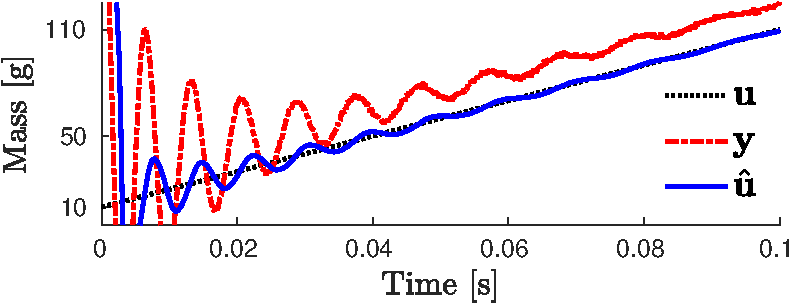
\includegraphics[width=1\columnwidth]{./ChapterRampInput/fig/Fig_2.pdf} 
\caption{ \label{fig:sensor_weight} The sensor transient response $y$ to an affine input excitation $u = at+b$ is processed by the estimation methods to estimate the parameters $a$ and $b$. In the figure we observe an example of the input estimate $\widehat{u}$ obtained with the subspace method. The input parameters are calculated from $\widehat{u}$ using linear regression.}
\end{figure}

In each simulation, the sensor response was perturbed with an independent realization of additive normally distributed measurement noise.
The added perturbation noise has signal-to-noise ratios (SNR) in the interval [20 dB, 60 dB], values that are realistic in practical applications.
The SNR is defined as the ratio of signal power to the noise power, that is equivalent to the root-mean-square value of the true signal to the variance of the perturbation noise, and in dB is given as

\begin{equation} \mathrm{SNR} = 20 \log_{10}{\dfrac{\dfrac{1}{T}\int\limits_0^T{\widebar{y}(t)^2 d t}}{\sigma_{\bm{\epsilon}}}} \end{equation}  


\subsection{Results of the subspace method}


The subspace method processed online the sensor transient response.
The first estimation was obtained with $2n+1$ samples.
The method updated recursively the value of the estimated parameters for each new collected sample, using the forgetting factor $\lambda$ listed in Table \ref{table:lambdas}.
In Figure \ref{fig:rele_dd_40dB_s1} we observe the relative errors of the estimates $\widehat{a}$ and $\widehat{b}$ obtained when SNR = 40 dB. 
The relative errors are smaller than 5 \% after 400 and 500 samples are processed, i.e., 0.04 s and 0.05 s, respectively.
As more samples are collected, the parameter estimation improves.
Figure \ref{fig:rele_SNR_dd_10000} shows the final value of the relative errors, found at $t=0.1$ s, for the different SNR values considered.
The relative errors are smaller than 2 \% regardless of the measurement noise level.

\begin{table}[h!]
\centering
\caption{The values of the forgetting factor $\lambda$ and the samples shift $\tau$ that configure the subspace method for the different values of SNR. These values were obtained after calibration of the method and fixed during the simulation study.}
\begin{tabular}{c| c c c c c} 
 \hline
 SNR \ [dB] & 20 & 30 & 40 & 50 & 60 \\ [0.5ex] 
 \hline
 $\lambda$ & 0.939 & 0.940 & 0.955 & 0.959 & 0.959 \\ % forgetting factor
 $\tau$ \  & 15 & 15 & 17 & 14 & 20 \\ [0.5ex] % [\mathrm{samples}]
 \hline
\end{tabular}
\label{table:lambdas}
\end{table}


\begin{figure}[!htbp]
\centering
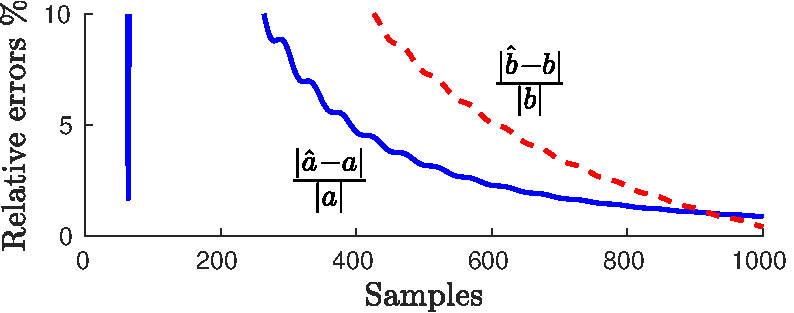
\includegraphics[width=1\columnwidth]{./ChapterRampInput/fig/Fig_3.pdf} 
\caption{ \label{fig:rele_dd_40dB_s1} The relative errors of the affine input parameters estimation decrease as the subspace method processes more samples. The relative errors of the estimates $\widehat{a}$ and $\widehat{b}$ are smaller than 5 \% after 400 and 500 samples, respectively ($T_s = 0.1$ ms). }
\end{figure}


\begin{figure}[!htbp]
\centering
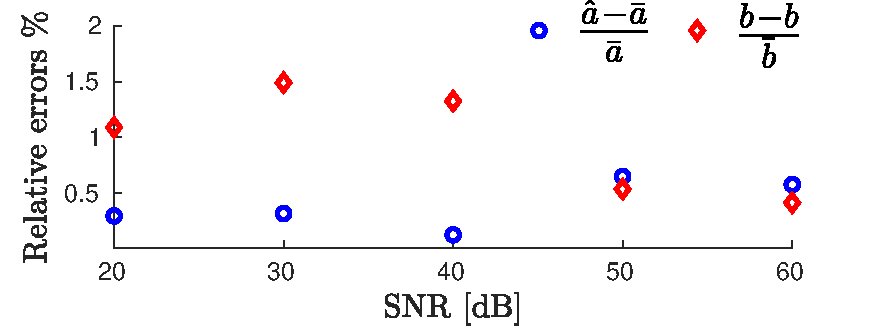
\includegraphics[width=1\columnwidth]{./ChapterRampInput/fig/Fig_4.pdf} 
\caption{ \label{fig:rele_SNR_dd_10000} The minimum value of the estimation relative errors obtained with the subspace method is less than 2  \% regardless of the SNR between 20 dB and 60 dB. }
\end{figure}

The Cram\'er-Rao lower bound (CRLB) of the errors-in-variables problem formulated by the subspace method was numerically computed for different sample size using Equation (\ref{eqn:FIM}).
The CRLB is the minimum variance that the estimates $\widehat{a}$ and $\widehat{b}$ can have.
The average of $10^4$ runs with independent noise realizations allows to find the empirical mean squared error (MSE) of the estimates, defined as
\begin{equation} \mathrm{MSE}_{\widehat{a}} = \left(b_{\mathrm{p}}\left( \widehat{a} \right) \right)^2 + v_{\mathrm{p}} \left( \widehat{a} \right), \quad \text{and} \quad  \mathrm{MSE}_{\widehat{b}} = ( b_{\mathrm{p}} ( \widehat{b} ) )^2 + v_{\mathrm{p}} ( \widehat{b} ), \end{equation}
where $b_{\mathrm{p}} \left( \widehat{a} \right)$ and $b_{\mathrm{p}} ( \widehat{b} )$ are the bias, and $v_{\mathrm{p}} \left( \widehat{a} \right)$ and $v_{\mathrm{p}} ( \widehat{b} )$ are the variances of the input parameters.
Figure \ref{fig:CRLB_MSE_ab_dd_40dB_MC_10000} shows that the mean squared errors $\mathrm{MSE}_{\hat{a}}$ and $\mathrm{MSE}_{\hat{b}}$ are near to their theoretical minimum $\mathrm{CRLB}_{a}$ and $\mathrm{CRLB}_{b}$ within two orders of magnitude, when SNR = 40 dB.
Figure \ref{fig:CRLB_MSE_SNR_ab_dd_MC_10000} shows the final value of the Cram\'er-Rao lower bounds and the empirical mean-squared errors, found at $t=0.1$ s, for the different SNR values considered.
Both $\mathrm{MSE}_{\hat{a}}$ and $\mathrm{MSE}_{\hat{b}}$ are less than one order of magnitude near to $\mathrm{CRLB}_a$ and $\mathrm{CRLB}_{b}$, respectively, for SNR $\leq 30$ dB.
The difference increases for larger SNR but the maximum is two orders of magnitude for SNR = 60 dB.

Table \ref{table:differentmasses} shows a comparative view of the estimation mean-squared-errors maximum values when the ramp that excites the sensor corresponds to different masses and time durations. 
For each mass and duration, the sensor responses were perturbed with measurement noise of SNR in the interval [20 dB, 60 dB].
The sensor parameters and sampling frequency are fixed and are the same described in the first paragraph of this section.
The maximum values of the MSE are mainly found at low SNR values between 20 and 40 dB.
The higher levels of noise increase the uncertainty of the estimation defined in terms of the MSE.
For fast ramp excitations, the MSE's increase considerably.
The used sampling frequency constrains the estimation method effectiveness for the ramp input duration of 0.05 s or shorter and there it is recommended to use  a higher sampling frequency that will reduce the estimation MSE.


\begin{figure}[!htbp]
\centering
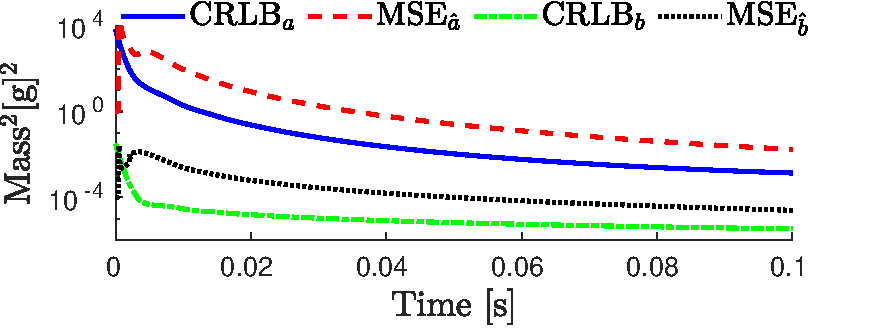
\includegraphics[width=1\columnwidth]{./ChapterRampInput/fig/Fig_5.pdf} 
\caption{ \label{fig:CRLB_MSE_ab_dd_40dB_MC_10000} When the SNR of the sensor response is 40 dB, the mean squared errors of the slope estimate $\widehat{a}$ and the interception estimate $\widehat{b}$, obtained by the subspace method, are two orders of magnitude above the theoretical minimum variance given by the Cram\'er-Rao lower bound.}
\end{figure}


\begin{figure}[!htbp]
\centering
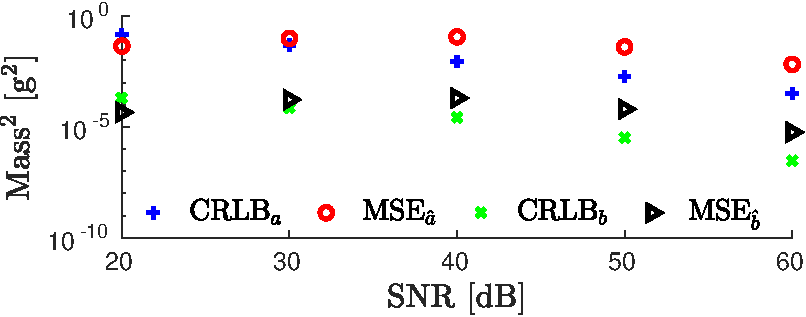
\includegraphics[width=1\columnwidth]{./ChapterRampInput/fig/Fig_6.pdf} 
\caption{ \label{fig:CRLB_MSE_SNR_ab_dd_MC_10000} The Cram\'er-Rao lower bounds of the estimates $\mathrm{CRLB}_a$ and $\mathrm{CRLB}_b$ determine the minimum uncertainty that can be achieved and increases with the measurement noise. 
The empirical mean squared errors $\mathrm{MSE}_{\hat{a}}$ and $\mathrm{MSE}_{\hat{b}}$ are near to the Cram\'er-Rao lower bounds within one order of magnitude for SNR smaller than 30 dB, and within two orders of magnitude for SNR between 40 dB and 60 dB. }
\end{figure}



\begin{table}[h!]
\centering
\caption{ The maximum values of the estimation mean squared errors observed when the subspace method processed the sensor transient responses caused by ramp excitations of masses 0.1, 0.3, 0.5, and 1.0 kg, that last 0.05, 0.1 and 0.5 s, with signal to noise ratios in the interval [20 dB, 60 dB] occur mainly at 40 dB and for lower SNR. There is an increment in the MSE values when the ramp excitation is faster.}
 
\begin{tabular}{L|L L L L} 
 \hline
 & \mathrm{Mass} & \\ [0.5ex] 
 \mathrm{Time} & 0.1 \ kg & 0.3 \ kg & 0.5 \ kg & 1.0 \ kg \\ 
 \hline
\multicolumn{1}{l|}{0.05 \ s} & \\
 \multicolumn{1}{r|}{\hspace{1mm} \mathrm{MSE}_{\hat{a}} \ [g^2]} & 3.5\mathrm{x}10^{0}_{(@40 \ \mathrm{dB})} & 13.5\mathrm{x}10^{0}_{(@50 \ \mathrm{dB})} & 3.8\mathrm{x}10^{0}_{(@20 \ \mathrm{dB})} & 8.3\mathrm{x}10^{0}_{(@50 \ \mathrm{dB})} \\ 
\multicolumn{1}{r|}{\hspace{1mm}\mathrm{MSE}_{\hat{b}} \ [g^2]} &  3.1\mathrm{x}10^{-3}_{(@40 \ \mathrm{dB})}  & 1.1\mathrm{x}10^{-2}_{(@40 \ \mathrm{dB})} & 1.1\mathrm{x}10^{-2}_{(@40 \ \mathrm{dB})} & 1.9\mathrm{x}10^{-2}_{(@60 \ \mathrm{dB})} \\
\multicolumn{1}{l|}{0.1 \ s} & \\
 \multicolumn{1}{r|}{\hspace{1mm}\mathrm{MSE}_{\hat{a}} \ [g^2]} & 3.1\mathrm{x}10^{-2}_{(@30 \ \mathrm{dB})} & 1.1\mathrm{x}10^{0}_{(@40 \ \mathrm{dB})} & 8.3\mathrm{x}10^{-1}_{(@60 \ \mathrm{dB})} & 1.3\mathrm{x}10^{0}_{(@50 \ \mathrm{dB})} \\
\multicolumn{1}{r|}{\hspace{1mm} \mathrm{MSE}_{\hat{b}} \ [g^2]} & 6.0\mathrm{x}10^{-5}_{(@30 \ \mathrm{dB})} & 1.2\mathrm{x}10^{-1}_{(@50 \ \mathrm{dB})} & 2.1\mathrm{x}10^{-2}_{(@40 \ \mathrm{dB})} & 3.7\mathrm{x}10^{-2}_{(@40 \ \mathrm{dB})} \\
\multicolumn{1}{l|}{0.5 \ s} & \\
 \multicolumn{1}{r|}{\hspace{1mm} \mathrm{MSE}_{\hat{a}} \ [g^2]} & 3.0\mathrm{x}10^{-2}_{(@20 \ \mathrm{dB})} & 3.0\mathrm{x}10^{-1}_{(@20 \ \mathrm{dB})} & 3.2\mathrm{x}10^{0}_{(@20 \ \mathrm{dB})} & 8.6\mathrm{x}10^{-2}_{(@20 \ \mathrm{dB})} \\
\multicolumn{1}{r|}{\hspace{1mm} \mathrm{MSE}_{\hat{b}} \ [g^2]} & 3.1\mathrm{x}10^{-5}_{(@50 \ \mathrm{dB})} & 9.8\mathrm{x}10^{-4}_{(@40 \ \mathrm{dB})} & 2.0\mathrm{x}10^{-5}_{(@50 \ \mathrm{dB})} & 1.7\mathrm{x}10^{-5}_{(@20 \ \mathrm{dB})} \\ [0.5ex] % [\mathrm{samples}]
 \hline
\end{tabular}
\
\label{table:differentmasses}
\end{table}


A numerical sensitivity analysis of the subspace method was conducted by adding uncertainty to ramp input generation and looking into the estimation results. 
The uncertainty $\sigma_{\mathrm{s}}$ of the speed in which the ramp increases, and the uncertainties of the input parameters, represented by $\sigma_{a,b}$, were selected to be 0\%, 5\% and 10\% of their true values.
A Monte Carlo simulation with $10^4$ runs was performed for each SNR and the maximum values of the estimation uncertainty are shown in Table \ref{table:dd_sensitivity}. 
According to these results, the input parameters uncertainties $\sigma_{a,b}$ affect more the uncertainty of the estimation than the speed uncertainty $\sigma_{\mathrm{s}}$. 
The parameter that is more affected by the input parameters uncertainty is the interception $\widehat{b}$, since the uncertainty of the slope $\widehat{a}$ is smaller.


\begin{table}[h!]
\centering
\caption{ A sensitivity analysis of the subspace method was conducted by adding uncertainty to the ramp input. The speed $\sigma_{\mathrm{s}}$, and the input parameters $\sigma_{\mathrm{s}}$ uncertainties are 0\%, 5\%, and 10\% of their true values. The table shows the maximum values of the estimates uncertainty. The speed uncertainty causes a smaller spread of the estimates than the input parameters uncertainty.}
 
\begin{tabular}{C| C C C} 
\hline  
& \sigma_{\mathrm{s}} \\ [0.5ex] 
\sigma_{{a},{b}}  & 0\% & 5\% & 10\% \\  
 \hline
 \multicolumn{1}{l|}{0\%} \\
 \multicolumn{1}{l|}{\hspace{2mm} \widehat{a} \ [\mathrm{kg/s}]} & 1.0 \pm 9.6 \%_{(@50 \ \mathrm{dB})} &  1.0 \pm 8.2 \%_{(@20 \ \mathrm{dB})} & 1.0 \pm 8.2 \%_{(@50 \ \mathrm{dB})} \\ 
 \multicolumn{1}{l|}{\hspace{2mm} \widehat{b} \ \mathrm{[g]}} & 10.0 \pm 10.3 \%_{(@20 \ \mathrm{dB})} & 9.9 \pm 14.2 \%_{(@30 \ \mathrm{dB})} &  10.0 \pm 21.7 \%_{(@60 \ \mathrm{dB})} \\ 
 \multicolumn{1}{l|}{5\%} \\
 \multicolumn{1}{l|}{\hspace{2mm} \widehat{a} \ [\mathrm{kg/s}]} & 1.0 \pm 9.7 \%_{(@50 \ \mathrm{dB})} & 1.0 \pm 11.3 \%_{(@20 \ \mathrm{dB})} & 1.0 \pm 8.0 \%_{(@50 \ \mathrm{dB})} \\  
 \multicolumn{1}{l|}{\hspace{2mm} \widehat{b} \ \mathrm{[g]}} & 10.0 \pm 22.4 \%_{(@50 \ \mathrm{dB})} & 10.0 \pm 33.2 \%_{(@30 \ \mathrm{dB})} & 9.9 \pm 16.6 \%_{(@50 \ \mathrm{dB})} \\ 
\multicolumn{1}{l|}{10\%} \\
\multicolumn{1}{l|}{\hspace{2mm} \widehat{a} \ [\mathrm{kg/s}]} & 1.0 \pm 20.3 \%_{(@40 \ \mathrm{dB})} & 1.0 \pm 22.0 \%_{(@50 \ \mathrm{dB})} & 1.0 \pm 17.7 \%_{(@40 \ \mathrm{dB})} \\    
 \multicolumn{1}{l|}{\hspace{2mm} \widehat{b} \ \mathrm{[g]}} & 9.9 \pm 46.8 \%_{(@40 \ \mathrm{dB})} & 9.8 \pm 58.8 \%_{(@50 \ \mathrm{dB})} & 9.9 \pm 41.6 \%_{(@40 \ \mathrm{dB})} \\ [0.5ex] 
\hline
\end{tabular}
\
\label{table:dd_sensitivity}
\end{table}



\subsection{Results of the maximum-likelihood method}
The maximum-likelihood (ML) method processed off-line the sensor transient response.
The ML method used the first 50 samples to initialize the optimization variables and updated the variables every $N = 1$ sample.
In Figure \ref{fig:rele_dd_40dB_s1} are shown the relative errors of the estimates $\widehat{a}$, $\widehat{b}$, $\widehat{x}_{\mathrm{ini,1}}$, and $\widehat{x}_{\mathrm{ini,2}}$.
The convergence of the ML estimates gives relative errors below 5 \% after three iterations.
The largest relative error observed is in the scale velocity $\widehat{x}_{\mathrm{ini,2}}$ estimate, which is more sensitive than the other optimization variables.

\begin{figure}[!htbp]
\centering
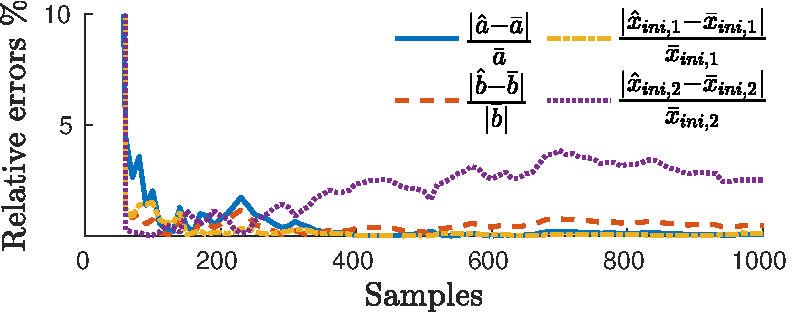
\includegraphics[width=1\columnwidth]{./ChapterRampInput/fig/Fig_7.pdf} 
\caption{ \label{fig:rele_lo_40dB_s10} The affine input parameters and the sensor initial conditions are estimated with the ML method. After three iterations the relative errors of the estimates are smaller than 5 \%.  }
\end{figure}

Using the analytic Jacobian and Equation (\ref{eqn:covOpt}), we computed the covariance of the estimate.
In Figure \ref{fig:cov_lo_40dB_s1} are shown the variances of the optimization variables taken from the diagonal of the covariance matrix. 
We can see that the variances of $\widehat{a}$ and $\widehat{b}$ decrease faster than the variances of $\widehat{x}_{\mathrm{ini,1}}$ and $\widehat{x}_{\mathrm{ini,2}}$ as more samples are processed.

\begin{figure}[!htbp]
\centering
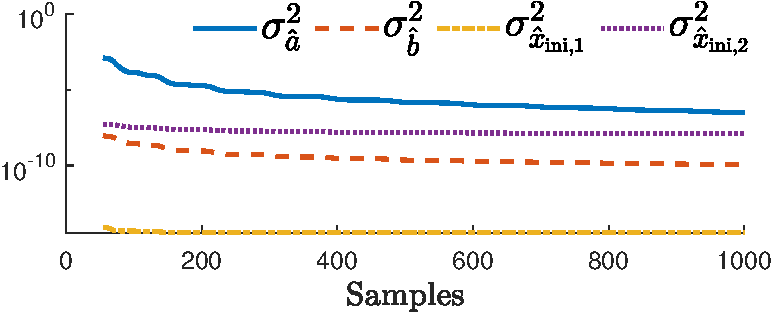
\includegraphics[width=1\columnwidth]{./ChapterRampInput/fig/Fig_8.pdf} 
\caption{ \label{fig:cov_lo_40dB_s1} The variances of the ML estimates are calculated using the information provided by the analytic Jacobian. The variances of the affine input parameters estimates decrease faster than the variances of the initial conditions estimates.  }
\end{figure}

The ML method is  computationally more expensive than the subspace method because the ML method simulates the response of a sensor model to optimize the input parameters and the sensor initial conditions.

A typical run of the ML method takes 30 s to complete.
With this execution time, the ML estimation can only be performed offline.
Nevertheless, the ML method objectives are to give the best estimation possible and to serve as a reference to assess the results of the other methods.
An efficient implementation of the ML method to make it feasible for real-time implementation is not trivial and requires additional research that is considered a topic for future research.

A numerical sensitivity analysis of the ML method was conducted by adding uncertainty to the ramp input, and to the parameters of the time-varying model. 
The ramp input was perturbed with uncertainty of the speed in which the ramp increases $\sigma_{\mathrm{s}}$, and with uncertainty on the input parameters $\sigma_{a,b}$. 
The perturbation uncertainty of the model parameters $m$, $d$, and $k$ is represented by $\sigma_{m,d,k}$. 
The perturbation uncertainty was simulated by adding normally distributed random noise with standard deviation equal to 0\%, 5\% and 10\% of the corresponding true values of the perturbed parameters.
A Monte Carlo simulation with $10^3$ runs was conducted for each SNR in the SNR innterval of interest, and in Table \ref{table:ml_sensitivity} are shown the maximum values of the observed estimation uncertainties. 
The results show that the speed uncertainty $\sigma_{\mathrm{s}}$ has a small impact on the estimation uncertainty.
On the contrary, the input parameters uncertainties $\sigma_{a,b}$, and the uncertainties of the model parameters $\sigma_{m,d,k}$ cause a large increment in the uncertainty of the estimation.

\begin{comment}

\begin{table}[h!]
\centering
\caption{ A sensitivity analysis of the ML method was conducted by adding uncertainty to ramp input, and to the model parameters. The perturbation uncertainty was selected with standard deviation of 0\%, 5\%, and 10\% of the parameters true values. The observed maximum estimation uncertainties are shown in the table. The speed uncertainty $\sigma_{\mathrm{s}}$ affects less the input estimation, but the uncertainties of the input parameters $\sigma_{a,b}$, and the model parameters $\sigma_{m,d,k}$ cause an increase of the estimation parameters spread around their mean values.}
 
\begin{tabular}{|C| C C C C|} 
\hline  
 &  & \sigma_{\mathrm{s}} \hspace{10mm} 0\% & \hspace{15mm} 5\% & \hspace{14mm} 10\% \\ [0.5ex] 
\hline
\sigma_{{a},{b}} \hspace{5.6mm} 0\% & \widehat{a} \ [\mathrm{kg/s}] & 0.999 \pm 0.7 \% \ (@20 \ \mathrm{dB}) & 1.0 \pm 0.7 \% \ (@20 \ \mathrm{dB}) & 0.999 \pm 0.4 \% \ (@30 \ \mathrm{dB}) \\ 
& \widehat{b} \ \mathrm{[g]} & \hspace{-1.75mm} 10.0 \pm 1.1 \% \ (@20 \ \mathrm{dB}) & 9.99 \pm 1.1 \% \ (@20 \ \mathrm{dB}) & 10.0 \pm 0.5 \% \ (@30 \ \mathrm{dB}) \\
& \widehat{x}_{\mathrm{ini,1}} \ \mathrm{[g]} & \hspace{-1.75mm} 0.1 \pm 0.6 \% \ (@40 \ \mathrm{dB}) & 0.1 \pm 0.6 \% \ (@20 \ \mathrm{dB}) &  0.1 \pm 0.2 \% \ (@30 \ \mathrm{dB}) \\
& \widehat{x}_{\mathrm{ini,2}} \ \mathrm{[g/s]} & \hspace{-1.75mm} 0.1 \pm 122 \% \ (@40 \ \mathrm{dB}) & 0.1 \pm 130 \% \ (@40 \ \mathrm{dB}) &  0.09 \pm 38 \% \ (@50 \ \mathrm{dB}) \\
  
\hspace{11.375mm} 5\% & \widehat{a} \ [\mathrm{kg/s}] & 1.0 \pm 9.0 \% \ (@50 \ \mathrm{dB}) & 0.997 \pm 5.2 \% \ (@40 \ \mathrm{dB}) & 1.0 \pm 5.6 \% \ (@40 \ \mathrm{dB}) \\  
& \widehat{b} \ \mathrm{[g]} & 9.88 \pm 25.4 \% \ (@50 \ \mathrm{dB}) & 9.97 \pm 5.2 \% \ (@20 \ \mathrm{dB}) & 10.01 \pm 4.7 \% \ (@40 \ \mathrm{dB}) \\ 
& \widehat{x}_{\mathrm{ini,1}} \ \mathrm{[g]} & \hspace{-1.75mm} 0.1 \pm 0.6 \% \ (@20 \ \mathrm{dB}) & 0.1 \pm 0.57 \% \ (@20 \ \mathrm{dB}) & 0.1 \pm 6.24 \% \ (@30 \ \mathrm{dB}) \\
& \widehat{x}_{\mathrm{ini,2}} \ \mathrm{[g/s]} & \hspace{-1.75mm} 0.1 \pm 116 \% \ (@40 \ \mathrm{dB}) & 0.09 \pm 128 \% \ (@40 \ \mathrm{dB}) & 0.11 \pm 115 \% \ (@40 \ \mathrm{dB}) \\
  
\hspace{9.595mm} 10\% & \widehat{a} \ [\mathrm{kg/s}] & 1.00 \pm 10.4 \% \ (@30 \ \mathrm{dB}) & 0.995 \pm 10.3 \% \ (@20 \ \mathrm{dB}) & 0.996 \pm 10.3 \% \ (@20 \ \mathrm{dB}) \\    
& \widehat{b} \ \mathrm{[g]} & 9.94 \pm 10.5 \% \ (@20 \ \mathrm{dB}) & 9.96 \pm 10.4 \% \ (@20 \ \mathrm{dB}) & 10.0 \pm 10.5 \% \ (@20 \ \mathrm{dB}) \\
& \widehat{x}_{\mathrm{ini,1}} \ \mathrm{[g]} & \hspace{-1.75mm} 0.1 \pm 0.6 \% \ (@20 \ \mathrm{dB}) & 0.1 \pm 0.6 \% \ (@20 \ \mathrm{dB}) & 0.1 \pm 0.6 \% \ (@20 \ \mathrm{dB}) \\
& \widehat{x}_{\mathrm{ini,2}} \ \mathrm{[g/s]} & \hspace{-1.75mm} 0.11 \pm 108 \% \ (@50 \ \mathrm{dB}) & 0.11 \pm 110 \% \ (@40 \ \mathrm{dB}) & 0.1 \pm 137 \% \ (@50 \ \mathrm{dB}) \\
 
\sigma_{{m},{d},{k}}  \hspace{2mm} 0\% & \widehat{a} \ [\mathrm{kg/s}] & 0.999 \pm 0.7 \% \ (@20 \ \mathrm{dB}) & 1.0 \pm 0.69 \% \ (@20 \ \mathrm{dB}) & 1.0 \pm 0.33 \% \ (@30 \ \mathrm{dB}) \\ 
& \widehat{b} \ \mathrm{[g]} & \hspace{-1.75mm} 10.0 \pm 1.1 \% \ (@20 \ \mathrm{dB}) & 10.0 \pm 1.13 \% \ (@20 \ \mathrm{dB}) &  10.0 \pm 0.46 \% \ (@30 \ \mathrm{dB}) \\
& \widehat{x}_{\mathrm{ini,1}} \ \mathrm{[g]} & \hspace{-1.75mm} 0.1 \pm 0.6 \% \ (@40 \ \mathrm{dB}) & 0.1 \pm 0.19 \% \ (@30 \ \mathrm{dB}) &  0.1 \pm 0.18 \% \ (@30 \ \mathrm{dB}) \\
& \widehat{x}_{\mathrm{ini,2}} \ \mathrm{[g/s]} & \hspace{-1.75mm} 0.1 \pm 122 \% \ (@40 \ \mathrm{dB}) & 0.1 \pm 130 \% \ (@40 \ \mathrm{dB}) & 0.09 \pm 38 \% \ (@50 \ \mathrm{dB}) \\
  
\hspace{11.375mm} 5\% & \widehat{a} \ [\mathrm{kg/s}] & 0.994 \pm 15.3 \% \ (@20g \ \mathrm{dB}) & 1.0 \pm 0.7 \% \ (@20 \ \mathrm{dB}) & 1.01 \pm 21.5 \% \ (@20 \ \mathrm{dB}) \\  
& \widehat{b} \ \mathrm{[g]} & 10.3 \pm 79.4 \% \ (@20 \ \mathrm{dB}) & 10.0 \pm 1.2 \% \ (@20 \ \mathrm{dB}) & 9.91 \pm 19.0 \% \ (@20 \ \mathrm{dB}) \\ 
& \widehat{x}_{\mathrm{ini,1}} \ \mathrm{[g]} & \hspace{-1.75mm} 0.1 \pm 0.2 \% \ (@30 \ \mathrm{dB}) & 0.1 \pm 0.6 \% \ (@20 \ \mathrm{dB}) & 0.1 \pm 0.19 \% \ (@20 \ \mathrm{dB}) \\
& \widehat{x}_{\mathrm{ini,2}} \ \mathrm{[g/s]} & \hspace{-1.75mm} 0.10 \pm 113 \% \ (@40 \ \mathrm{dB}) & 0.1 \pm 119 \% \ (@40 \ \mathrm{dB}) & 0.11 \pm 323 \% \ (@30 \ \mathrm{dB}) \\
  
\hspace{9.595mm} 10\% & \widehat{a} \ [\mathrm{kg/s}] & 1.01 \pm 22 \% \ (@30 \ \mathrm{dB}) & 1.01 \pm 16.0 \% \ (@30 \ \mathrm{dB}) & 0.987 \pm 28 \% \ (@50 \ \mathrm{dB}) \\    
& \widehat{b} \ \mathrm{[g]} & 0.1 \pm 26 \% \ (@30 \ \mathrm{dB}) & 9.93 \pm 14.8 \% \ (@30 \ \mathrm{dB}) & 10.4 \pm 93 \% \ (@50 \ \mathrm{dB}) \\ 
& \widehat{x}_{\mathrm{ini,1}} \ \mathrm{[g]} & \hspace{-1.75mm} 0.1 \pm 0.6 \% \ (@20 \ \mathrm{dB}) & 0.1 \pm 0.6 \% \ (@20 \ \mathrm{dB}) &  0.1 \pm 0.6 \% \ (@20 \ \mathrm{dB}) \\
& \widehat{x}_{\mathrm{ini,2}} \ \mathrm{[g/s]} & \hspace{-1.75mm} 0.1 \pm 121 \% \ (@40 \ \mathrm{dB}) & 0.09 \pm 136 \% \ (@40 \ \mathrm{dB}) & 0.11 \pm 111 \% \ (@40 \ \mathrm{dB}) \\
[0.5ex] 
\hline
\end{tabular}
\
\label{table:ml_sensitivity}
\end{table}

\end{comment}



\subsection{Results of the time-varying filter}

We fixed the frequency lower value $f_l=0.01$ Hz and the base $\beta = 0.01$. 
The upper value $f_u$ and the decay rate $\alpha$ were found using optimization (\ref{eqn:tv_optim}). 
We chose the values $\mu_{\mathrm{spec}}=0.5$ and $\sigma_{\mathrm{spec}}=0.24$ as they are specified in the OIML recommendation \cite{OIML_R51_1} for a mass of 100 g measured in a conveyor belt.
The optimized values of the frequency upper value and the decay rate, using a dataset of 100 transient responses, were $f_u = 26.94$ Hz and $\alpha = 5.71$.

Figure \ref{fig:rele_tv_40dB_s1} shows the relative errors of the estimates $\widehat{a}$ and $\widehat{b}$ computed with the TV filter after processing the sensor transient response.
The relative error of the slope estimate is below 5 \% after 300 samples but the relative error of the interception estimate is near 10 \%.
The convergence rate of the estimate $\widehat{a}$ was similar to that of the subspace method.

\begin{figure}[!htbp]
\centering
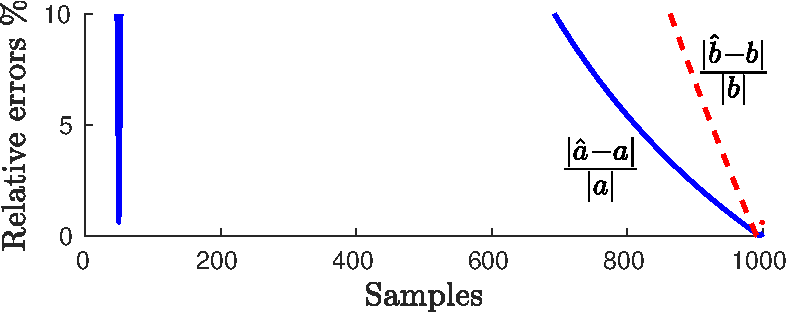
\includegraphics[width=1\columnwidth]{./ChapterRampInput/fig/Fig_9.pdf} 
\caption{ \label{fig:rele_tv_40dB_s1} The relative errors of the time-varying filter estimation converge slower than with the subspace method. 
The relative errors of $\widehat{a}$ and $\widehat{b}$ are smaller than 5 \% only after 800 and 950 samples, respectively.
With the subspace method the relative errors are below 5 \% after 400 and 500 samples. }
\end{figure}



\subsection{Discussion of the observed results}

The subspace method obtains an estimation of the affine input parameters with a recursive least squares solution of a structured errors-in-variables problem.
Updating the parameter estimates without matrix inversion simplifies the method implementation on digital signal processors of low cost.
The price we pay by computing the least squares solution of an errors-in-variables problem is an increase in the bias of the estimates.
Nevertheless, the empirical mean squared errors of the estimates are at most two orders of magnitude larger than the Cram\'er-Rao lower bound, meaning that the estimates uncertainty is low, even when the SNR is lower than 40 dB.


The proposed subspace method is a general method that can be used in different applications, with realistic signal-to-noise ratios. 
It is suitable not only for mass measurements.
The weighing example shows that the subspace method can be used even when the measurement system is linear time-varying.

It was shown that the time-varying (TV) compensation filter can be modified to estimate the mass only from the increasing section of the saturated ramp, without the need of processing the saturation part.
The modified TV filter can be implemented in real-time as the subspace method after a previous off-line coefficients optimization stage with sensor measured data.
Nevertheless, the estimation results of the subspace method are better than the TV filter since they are twice as fast and one order of magnitude more acurate.

The subspace method can estimate the affine input parameters from the sensor response using few parameters, the sensor order $n$, the sensor static gain $\gamma$, and the RLS forgetting factor $\lambda$.
The subspace method does not necessarily requires optimization of $\lambda$ using a dataset of measured sensor responses.
It is required to tune $\lambda$ online during the calibration of the system and later $\lambda$ remains fixed during the measurements.

The results of the sensitivity analysis show how the uncertainty of the subspace method estimates is affected when the ramp input is subject to perturbation.
The impact on the uncertainty on the slope $\widehat{a}$ and the interception $\widehat{b}$ parameters is different.
The ramp speed uncertainty $\sigma_{\mathrm{s}}$ is added to the uncertainty of the parameter $\widehat{b}$, but does not contribute to the uncertainty of the parameter $\widehat{a}$.
On the other hand, the ramp parameters uncertainty ramp speed uncertainty $\sigma_{a,b}$ is added to the uncertainty of the estimates of both parameters $\widehat{a}$ and $\widehat{b}$.
This is not surprising since the estimation parameters are linked to the ramp input parameters.

The maximum-likelihood (ML) method is an approach that requires larger computational resources.
This is an iterative method and in each iteration computes a simulation of a dynamic system followed by the evaluation of the residual error Jacobian matrix.
The advantage of the ML method is that we can estimate simultaneously sensor parameters and the initial conditions of the sensor.
In the weighing case presented as an illustrative example it was not possible to incorporate other parameters of the sensor because they are not identifiable.
According to the estimation relative errors, that are lower than 0.01 after 100 samples, from there on the ML method estimates are near to the true values and we may not require to run the method along all the measurement period.
With only the first 100 samples we have an accurate parameter estimation and variance assessment.

However, the main drawback of the ML method that prevents online implementations is the required computational power to iteratively simulate the response of a sensor model.
It takes an average of 30 s to complete an estimation with the ML method, and this time is too large for fast changing inputs.
The development of an efficient ML method, suitable for real-time implementation, is not straightforward, and is proposed for future research.

The results of the sensitivity analysis of the ML method show that the uncertainty of the ramp input speed $\sigma_{\mathrm{s}}$ does not have an impact on the estimates uncertainty.
Similar to the subspace case, the uncertainty of the ramp input parameters $\sigma_{a,b}$ is additive to the uncertainty of the estimated parameters $\widehat{a}$ and $\widehat{b}$, but does not contribute to the uncertainty of the first element of the initial conditions.
On the other hand, the estimates uncertainty is affected by the perturbation on the model parameters $\sigma_{m,d,k}$.
It is observed that the uncertainty of the estimated parameters $\widehat{a}$ and $\widehat{b}$ increases two and three times the uncertainty of the model parameters.
This implies that we need to have an accurate model of the dynamic system to have a small uncertainty on the estimated input parameters.
Unfortunately, the uncertainty of the second element of the inital conditions is always very high and this is not because of the perturbation of the ramp speed or the model parameters. 
This issue requires more investigation to see if it is due the identifiability of the parameter in the particular example we have.


\section{Conclusions}

An adaptive subspace method was proposed for the estimation of affine input parameters given the measurement of the caused sensor transient response. 
The subspace estimation method is a recursive method that allows online implementation.
This method tracks the input of a system, using exponential forgetting, to process the system response.
The subspace method is model-free and estimates directly the input parameters without identifying a sensor model.
Therefore, it can be applied to the measurement of different physical magnitudes.
In the specific weighing example described in the manuscript, the input is an affine function.
The method is also applicable when the sensor is time-varying.
The subspace method is computationally cheap, simple and suitable for implementation on digital signal processor of low computational power. 

A maximum-likelihood estimator based on local optimization was designed to obtain a comparative reference for the other methods.
The maximum-likelihood method estimates the affine input parameters and also model parameters and the sensor's initial conditions.
This method simulates, in a receding horizon scheme, the response of a sensor model to estimate the input and minimizes the sum of the squares of the residual between the measured and the estimated responses.
The main drawback of the maximum-likelihood method is its computational cost and efficient implementation of the method is left for future work.

A linear time-invariant weighing system is used as an test example for the estimation methods.
The weighing system becomes time-varying when an affine input excites the system.
The estimation methods are compared in a simulation study where the time-varying sensor response is perturbed by measurement noise, that is assumed white of zero mean and known variance.
The subspace method results are also compared to those of an existing digital time-varying filter.
The coefficients of the time-varying filter require offline optimization.
The estimation results obtained with the subspace method converges two times faster and is one order of magnitude smaller than those obtained with the time-varying filter.
The empirical mean squared errors of the subspace method estimation is two orders of magnitude larger than the theoretical minimum given by the Cram\'er-Rao Lower bound.

Future work of this research is the practical implementation of the subspace method for real-time measurements.

\newpage


%\part{Figures of merit for~characterizing nonlinear~devices}\label{part:PA}


\addtocontents{toc}{\vspace{2em}} %!TEX root = ..\Thesis.tex
\glsresetall

\chapter[Conclusions and future work]{Conclusions and \linebreak future work} \label{chap:concl}

\vfill{}

%In this final chapter, I first summarize the contributions made in the thesis. Then, I propose some possible further improvements to extend this work in future research.

%\newpage
%\section*{Conclusions}

In this thesis is described a process to validate a signal processing method for practical applications.
The signal processing method takes the transient step response of a linear time-invariant sensor and provides an estimation of the level of the originating step input.
The signal processing method is a subspace data-driven estimation method and constitutes an alternative to the common sensor response processing approaches based in compensation filters.
Contrary to the compensation filters, this data-driven estimation method is model independent, and improves the estimation time because the model parameters do not have to be estimated neither previously nor simultaneously to the input estimation.
The improvement in speed estimation makes the data-driven method suitable for online applications, such as real-time measurements.


In order to convince the metrology community of the benefits and effectiveness of the data-driven method, is was pending to quantify the uncertainty of is resulting estimation.
The uncertainty of the this method remained unknown because is not straightforward to determine the statistical propertines of its input estimate.
The data-driven method formulates a minimization problem that is a structured and correlated errors-in-variables (EIV) problem.
In order to facilitate the practical online applications, the solution to the minimization problem is proposed in terms of the recursive least-squares (LS) estimator.
The structure and the correlation made necessary to conduct research towards the the first and second moments statistical moments of the LS solution.


The first part of the research reported in this thesis deals with the determination of the mean value and the covariance that the LS estimator has when it solves a structured and correlated EIV problem.
The Taylor series expansion of the LS solution permits the study of the expected value of the LS estimate.
The series expansion considers the structure of the regression matrix and the correlation between the regression matrix and the regressor.
It was found that the element-wise treatment is not a strict requisite for the statistical analysis, since a matrix form treatment is possible.
As a result, the statistical analysis yielded expressions that approximate the bias and the covariance of the LS estimate, for different amount of samples and perturbation levels.
These expressions also help to understand the impact that the different matrix structures and the correlation bring into EIV problems and their solutions.



The LS bias and covariance predictions were validated first by Monte Carlo simulations. 
In the simulations, the empirical statistical moments of the LS estimation were compared to the predictions.
The simulations were performed with an extensive set of values in the workspace of the sample size of the step response observations, and the perturbation levels.
The learning obtained from the simulation results are the operating conditions in which the estimation method is effective.
The operation conditions were the data-driven estimation method was found to be effective include a region of signal-to-noise (SNR) near to 40 dB, were many real-life applications are currently used.
This is a positive indication for the usability of the method in metrology.
Another encouraging result is that the mean squared error of the data-driven method estimate is considerably near to the minimal theoretical variance that is defined by the Cram\'er-Rao lower bound of the formulated EIV problem.




Experimental research in a series of experimental measurements completes the validation of the data-driven step input estimation method.
The temperature and mass measurements are adequate for testing the implementation of the method.
These two physical magnitudes are demanded applications in scientific and industrial fields.
The mass measurement demands more effort from the step input estimation method in a real-life application.
Mass measurement sensors are easily perturbed by vibrations of the environment.
Furthermore, the mechanical constructions of the weighing sensors increase the order complexity of the sensor model.
A non-surprising observation in the experimental mass measurements implementation is that the measurement noise collected from the weighing sensor is not Gaussian white noise.
Moreover, the weighing sensor used, a load cell sensor, has a high order, in theory infinite. 
Nevertheless, the data-driven step input estimation method performed very well under these conditions. 
The estimation method showed robustness against non-white noise and provided acceptable results for system orders selected between 5 and 7. 




A third aspect of the conducted research included the exploration for the estimation of other input models with signal processing methods. 
The affine input is one input model that is one complexity level higher than the step input and then it was selected to be considered for further study.
The recursive LS estimator is a specific case of the exponentially weighted recursive LS (EWRLS), that is able to process the affine input response to estimate the actual input.
To do this, the EWRLS estimator uses a tuning parameter that selects the data samples.
During the study of the data-driven method adaptation for the affine input, it was observed that the affine input applied to a weighing sensor turns the LTI sensor into a time-varying (TV) sensor. 
Thus, the estimation problem became more interesting.
The adaptive affine input estimation method was simulated under different assumptions and showed robustness when processing time-varying sensor responses.
To compare the results of this adaptive method, a maximum-likelihood (ML) estimator based on local optimization, and a previously reported digital time-varying filter were implemented.
The adaptive affine input estimation method outperformed the time-varying filter by presenting lower estimation time, and the ML method by requiring less computational effort. 


\section*{Future work}

The use of model independent signal processing methods is a research field that surely will produce interesting results in the near future. 
With the increasing power of digital signal processors, the design of new methods is an opportunity that cannot be disregarded.

The data-driven method studied in this thesis is one example of an alternative to dynamic measurements under a different paradigm.
With respect to this method, one conclusion of the analysis presented can be that the data-driven step input estimation method is not statistically efficient because the estimation shows bias.
A topic for future research is the efficiency increase, perhaps by designing fast and optimal estimators for structured and correlated EIV problems. 

On the other hand, for model-based estimation methods, such as the described ML method that has a high computational cost, there is a need also for efficient implementations to enable online optimization in receding-horizon schemes. 
With such efficient methods, the practical implementation of the ML methods can become feasible for real-time measurements.


\newpage


\begin{comment}
\section{Conclusions - Statistical analysis}

 We conducted a statistical analysis of a structured errors-in-variables (EIV) estimation problem with correlation to find the first and second moments of its least-squares solution.
This estimation problem occurs in metrology when we estimate the value of a measurand directly from the sensor transient response.
The data-driven estimation of the physical quantity is formulated as a structured EIV problem with correlation that uses the observed transient response to construct both the regression matrix and the regressor.
The real-time implementation of the method uses a recursive least-squares algorithm that is simple and has low computational complexity.
The assessment of the uncertainty is done using the estimate bias and variance.

The conducted statistical analysis produced expressions that predict the estimate bias and variance for given sample size and perturbation level of the observed response.
The Monte Carlo simulation validated the predictions.
We compared the results of solving an unstructured and uncorrelated EIV problem with a structured and correlated EIV problem to understand how the structure and the correlation impacts in the estimation.
We found that the predictions in the structured case are more susceptible to perturbations.
This is due to the two approximations involved, a second-order Taylor series expansion of the estimate, and the substitution of perturbed data on the prediction expressions.
The relative error results indicate that the estimate bias, and variance are predicted using the derived expressions, and the observed data.
The mean squared error of the estimate is close to the results of the maximum likelihood estimate given by the Cram\'er-Rao lower bound.

The bias and variance can be accurately predicted, provided that the Taylor series expansion is valid.
This constraint has to be taken into account to ensure the effectiveness of the method in practical applications.
In the example, it was observed that when the SNR lies outside the validity region, the bias and variance estimation was at most three times larger than the empirical values.

The methodology presented in this paper can be applied to estimate the uncertainty of the solutions to other structured EIV problems.
The bias and variance expressions obtained after the statistical analysis depend on each specific structure.


\section{Conclusions - Experimental validation}

In this paper we investigated the statistical properties of a data-driven step input estimation method in a real-life application.
The step input estimation method is a structured and correlated errors-in-variables problem that is solved with recursive least-squares.
A statistical analysis was conducted using the ordinary least-squares condensed notation. 
This statistical analysis of the input estimate provides expressions that approximate the estimation bias and variance assuming that the measurement noise is Gaussian white noise. 
The variance approximation is useful to assess the uncertainty of the input estimate.
In simulation we observed that the mean squared error of the input estimate is close to the theoretical minimum that uses the Cram\'er-Rao lower bound for biased estimators.
Since the data-driven step input estimation method is not statistically efficient, there is room for improvement. This is a topic for future research.
In the practical experiments, the measurement noise is not white.
The noise variance obtained from the sensor steady state response underestimates the measurement noise variance, that was observed 5 dB larger in the power spectrum due to nonlinearities of the sensor.
Considering this difference in the measurement noise variance, we introduced a conservative bound of the measurement noise variance so that the first and second moments of the input estimate are more accurately predicted.
Using the variance approximation, we can assess the uncertainty of the input estimate with respect to the number of samples processed by the data-driven step input estimation method.
The step input estimation method is useful in practical applications where the whiteness assumption of the measurement noise is not fulfilled. 

\section{Conclusions - Ramp input}

An adaptive subspace method was proposed for the estimation of affine input parameters given the measurement of the caused sensor transient response. 
The subspace estimation method is a recursive method that allows online implementation.
This method tracks the input of a system, using exponential forgetting, to process the system response.
The subspace method is model-free and estimates directly the input parameters without identifying a sensor model.
Therefore, it can be applied to the measurement of different physical magnitudes.
In the specific weighing example described in the manuscript, the input is an affine function.
The method is also applicable when the sensor is time-varying.
The subspace method is computationally cheap, simple and suitable for implementation on digital signal processor of low computational power. 

A maximum-likelihood estimator based on local optimization was designed to obtain a comparative reference for the other methods.
The maximum-likelihood method estimates the affine input parameters and also model parameters and the sensor's initial conditions.
This method simulates, in a receding horizon scheme, the response of a sensor model to estimate the input and minimizes the sum of the squares of the residual between the measured and the estimated responses.
The main drawback of the maximum-likelihood method is its computational cost and efficient implementation of the method is left for future work.

A linear time-invariant weighing system is used as an test example for the estimation methods.
The weighing system becomes time-varying when an affine input excites the system.
The estimation methods are compared in a simulation study where the time-varying sensor response is perturbed by measurement noise, that is assumed white of zero mean and known variance.
The subspace method results are also compared to those of an existing digital time-varying filter.
The coefficients of the time-varying filter require offline optimization.
The estimation results obtained with the subspace method converges two times faster and is one order of magnitude smaller than those obtained with the time-varying filter.
The empirical mean squared errors of the subspace method estimation is two orders of magnitude larger than the theoretical minimum given by the Cram\'er-Rao Lower bound.

Future work of this research is the practical implementation of the subspace method for real-time measurements.
\end{comment}



%%%%%%%%%%%%%%%%%%%%%%%%%%%%%  Start appendix
 

\appendix
\addtocontents{toc}{\vspace{0em}} %!TEX root = ..\Thesis.tex
\glsresetall

\chapter{Appendices }\label{chap:Appendices}
% \begin{quote}
% \emph{The results of this chapter are based on the \cite{VanNechel2018}.}\vfill{}
% \end{quote}
\vfill{}


 
 
\section{Appendix - Jacobians in Ramp input ML estimation}


The entries of the Jacobian matrix are the first order partial derivatives of the residual error $\mathbf{r}$ with respect to the optimization variables.
The state space representation of the weighing model allows to find the analytical expression of the Jacobian.
The partial derivative of the residual error $\mathbf{r}$ with respect to the optimization variable $a$ is 
\begin{equation} \mathbf{J}_a=\dfrac{\partial \mathbf{r}}{\partial a} = \dfrac{\partial \widehat{y}}{\partial a} = \begin{bmatrix} 1 & 0  \end{bmatrix} \dfrac{\partial \mathbf{x}}{\partial a} = \begin{bmatrix} 1 & 0  \end{bmatrix} \mathbf{x}_a \end{equation}
where we use $\mathbf{x}_a = \partial \mathbf{x}/ \partial a$ to simplify the notation. 
Now, from the derivative of the state equation, we have
\begin{equation} \begin{aligned} 
    & \dot{\mathbf{x}}_a = \begin{bmatrix} 0 & 1 \\ \frac{-k_{\mathrm{s}}}{a t + b + m} & \frac{-(a + k_{\mathrm{d}})}{a t + b + m} \end{bmatrix} \mathbf{x}_a 
    + \begin{bmatrix} 0 & 0 \\ \frac{k_{\mathrm{s}} t}{(a t + b + m)^2} & \frac{k_{\mathrm{d}} t - b - m}{(a t + b + m)^2} \end{bmatrix} \mathbf{x} 
    - \frac{t \ \delta(t)}{(a t + b + m)^2} \mathbf{x}_{\text{ini}}   . 
\end{aligned} \end{equation}
Then, the partial derivative of the error $\mathbf{r}$ with respect to the optimization variable $a$ results in an additional dynamic system.

By repeating the procedure, we obtain the partial derivatives with respect to $b$ as follows: 
\begin{equation} \begin{aligned} 
    & \dot{\mathbf{x}}_b = \begin{bmatrix} 0 & 1 \\ \frac{-k_{\mathrm{s}}}{a t + b + m} & \frac{-(a + k_{\mathrm{d}})}{a t + b + m} \end{bmatrix} \mathbf{x}_b 
    + \begin{bmatrix} 0 & 0 \\ \frac{k_{\mathrm{s}}}{(a t + b + m)^2} & \frac{a+k_{\mathrm{d}}}{(a t + b + m)^2} \end{bmatrix} \mathbf{x} 
 - \frac{\delta(t) }{(a t + b + m)^2}  \mathbf{x}_{\text{ini}} ,
 \\ & \mathbf{J}_b = \begin{bmatrix} 1 & 0 \end{bmatrix} \mathbf{x}_b . 
\end{aligned} \end{equation}
The partial derivatives of the error $\mathbf{r}$ with respect to the initial conditions yield the following two Jacobians
\begin{equation} \begin{aligned}
    & \dot{\mathbf{x}}_{\mathbf{x}_{\text{ini,1}}} = \begin{bmatrix} 0 & 1 \\ \frac{-k_{\mathrm{s}}}{a t + b + m} & \frac{-(a + k_{\mathrm{d}})}{a t + b + m} \end{bmatrix} \mathbf{x}_{\mathbf{x}_{\text{ini,1}}} + \begin{bmatrix} \frac{\delta(t)}{a t + b + m} \\ 0 \end{bmatrix} , \\
    & \mathbf{J}_{\mathbf{x}_{\text{ini,1}}} = \begin{bmatrix} 1 & 0 \end{bmatrix} \mathbf{x}_{\mathbf{x}_{\text{ini,1}}}.
\end{aligned} \end{equation}
and
\begin{equation} \begin{aligned}
    & \dot{\mathbf{x}}_{\mathbf{x}_{\text{ini,2}}} = \begin{bmatrix} 0 & 1 \\ \frac{-k_{\mathrm{s}}}{a t + b + m} & \frac{-(a+k_{\mathrm{d}})}{a t + b + m} \end{bmatrix} \mathbf{x}_{\mathbf{x}_{\text{ini,2}}} + \begin{bmatrix} 0 \\ \frac{\delta(t)}{a t + b + m} \end{bmatrix} ,  \\
    & \mathbf{J}_{\mathbf{x}_{\text{ini,2}}}=\begin{bmatrix} 1 & 0 \end{bmatrix} \mathbf{x}_{\mathbf{x}_{\text{ini,2}}}.
\end{aligned} \end{equation}

The Jacobian matrix is constructed using the responses of the additional dynamic systems  
\begin{equation} \begin{aligned} \mathbf{J} &= \begin{bmatrix} \mathbf{J}_a & \mathbf{J}_b & \mathbf{J}_{\mathbf{x}_{\text{ini,1}}} & \mathbf{J}_{\mathbf{x}_{\text{ini,2}}} \end{bmatrix} \end{aligned} \end{equation}




\section{Appendix - Derivation of bias and covariance expressions.}

The bias and covariance of the least-squares (LS) estimate (\ref{eqn:xhatexp}) are obtained using the mathematical expectation in the definitions (\ref{eqn:biasdef}) and (\ref{eqn:covdef}).
For an unstructured and uncorrelated EIV problem, the expected value, and the covariance of $\widehat{\mathbf{x}}$ are approximated by
\begin{equation} \begin{aligned} \mathbb{E} \left\{ \widehat{\mathbf{x}} \right\} & \approx \mathbf{x}  + \mathbf{Q}^{-1} \mathbb{E} \left\{ \mathbf{K}^\top \mathbf{E} \mathbf{Q}^{-1} \mathbf{K}^\top \mathbf{E} + \mathbf{E}^\top \mathbf{K} \mathbf{Q}^{-1} \mathbf{K}^\top \mathbf{E} - \mathbf{E}^\top \mathbf{E}  \right\} \mathbf{x}, \quad \text{and}  \\ 
\mathbf{C} \left( \widehat{\mathbf{x}} \right)  & \approx \mathbf{x} \mathbf{x}^\top + \mathbf{Q}^{-1} \mathbb{E} \left\{ \mathbf{K}^\top \bm{\epsilon} \bm{\epsilon}^\top \mathbf{K} + \mathbf{K}^\top \mathbf{E} \mathbf{x} \mathbf{x}^\top \mathbf{E}^\top \mathbf{K} \right\} \mathbf{Q}^{-1} \\ 
& + \mathbf{Q}^{-1} \mathbb{E} \left\{ \mathbf{K}^\top \mathbf{E} \mathbf{Q}^{-1} \mathbf{K}^\top \mathbf{E} + \mathbf{E}^\top \mathbf{K} \mathbf{Q}^{-1} \mathbf{K}^\top \mathbf{E} - \mathbf{E}^\top \mathbf{E} \right\} \mathbf{x} \mathbf{x}^\top \\
& + \mathbf{x} \mathbf{x}^\top \mathbb{E} \left\{ \mathbf{E}^\top \mathbf{K} \mathbf{Q}^{-1} \mathbf{E}^\top \mathbf{K} + \mathbf{E}^\top \mathbf{K} \mathbf{Q}^{-1} \mathbf{K}^\top \mathbf{E} - \mathbf{E}^\top \mathbf{E} \right\} \mathbf{Q}^{-1} - \mathbb{E} \left\{ \widehat{\mathbf{x}} \right\} \mathbb{E} \left\{ \widehat{\mathbf{x}} \right\}^\top , \label{eqn:EC_Eu} \end{aligned} \end{equation} 
where we have considered the second order Taylor series approximation (\ref{eqn:TseriesExp}), and we have removed the terms of zero expected value, and the terms of order higher than 2.
After an elementwise evaluation of the corresponding expected values in (\ref{eqn:EC_Eu}), the expressions result in 
\begin{equation} \begin{aligned} \mathbb{E} \left\{ \widehat{\mathbf{x}} \right\} & \approx \mathbf{x}  + \mathbf{b}_{\mathrm{p}} \left( \widehat{\mathbf{x}} \right) = \mathbf{x}  +  \sigma_{\mathbf{E}}^2 \mathbf{Q}^{-1} \left( 2\mathbf{I} + 2n\mathbf{I} - T \mathbf{I} \right) \mathbf{x} , \quad \text{and} \\ 
\mathbf{C}_{\mathrm{p}} \left( \widehat{\mathbf{x}} \right) & \approx \sigma_{\bm{\epsilon}}^2 \ \mathbf{Q}^{-1} + \sigma_{\mathbf{E}}^2 \ \mathrm{trace} \left( \mathbf{x} \mathbf{x}^\top \right) \mathbf{Q}^{-1} - \sigma_{\mathbf{E}}^4 \left( 2 + 2n - T \right)^2 \ \mathbf{Q}^{-1} \mathbf{x} \mathbf{x}^\top \mathbf{Q}^{-1} , \end{aligned} \end{equation}
from where equations (\ref{eqn:biasEu}) and (\ref{eqn:varEu}) are obtained.

On the other hand, due to the correlation, the expressions that approximate the expected value of the LS estimate of the structured and EIV problem (\ref{eqn:min_ls}) have a different form:
\begin{equation} \begin{aligned} \mathbb{E} \left\{ \widehat{\mathbf{x}} \right\} & \approx \mathbf{x}  +  \mathbf{Q}^{-1} \mathbb{E} \left\{ \mathbf{K}^\top \mathbf{E} \mathbf{Q}^{-1} \mathbf{K}^\top \mathbf{E} + \mathbf{E}^\top \mathbf{K} \mathbf{Q}^{-1} \mathbf{K}^\top \mathbf{E} - \mathbf{E}^\top \mathbf{E}  \right\} \mathbf{x} \\ 
& + \mathbf{Q}^{-1} \mathbb{E} \left\{ \mathbf{E}^\top \bm{\epsilon} - \mathbf{K}^\top \mathbf{E} \mathbf{Q}^{-1} \mathbf{K}^\top \bm{\epsilon} - \mathbf{E}^\top \mathbf{K} \mathbf{Q}^{-1} \mathbf{K}^\top \bm{\epsilon} \right\} , \quad \text{and}  \\ 
\mathbf{C} \left( \widehat{\mathbf{x}} \right)  & \approx \mathbf{x} \mathbf{x}^\top + \mathbf{Q}^{-1} \mathbb{E} \left\{ \mathbf{K}^\top \bm{\epsilon} \bm{\epsilon}^\top \mathbf{K} + \mathbf{K}^\top \mathbf{E} \mathbf{x} \mathbf{x}^\top \mathbf{E}^\top \mathbf{K} - \mathbf{K}^\top \mathbf{E} \mathbf{x} \bm{\epsilon}^\top \mathbf{K} - \mathbf{K}^\top \bm{\epsilon} \mathbf{x}^\top \mathbf{E}^\top \mathbf{K} \right\} \mathbf{Q}^{-1}  \\
& + \mathbf{Q}^{-1} \mathbb{E} \left\{ \mathbf{K}^\top \mathbf{E} \mathbf{Q}^{-1} \mathbf{K}^\top \mathbf{E} + \mathbf{E}^\top \mathbf{K} \mathbf{Q}^{-1} \mathbf{K}^\top \mathbf{E} - \mathbf{E}^\top \mathbf{E} \right\} \mathbf{x} \mathbf{x}^\top \\
& + \mathbf{x} \mathbf{x}^\top \mathbb{E} \left\{ \mathbf{E}^\top \mathbf{K} \mathbf{Q}^{-1} \mathbf{E}^\top \mathbf{K} + \mathbf{E}^\top \mathbf{K} \mathbf{Q}^{-1} \mathbf{K}^\top \mathbf{E} - \mathbf{E}^\top \mathbf{E} \right\} \mathbf{Q}^{-1} - \mathbb{E} \left\{ \widehat{\mathbf{x}} \right\} \mathbb{E} \left\{ \widehat{\mathbf{x}} \right\}^\top \\ 
& + \mathbf{Q}^{-1} \mathbb{E} \left\{ \mathbf{E}^\top \bm{\epsilon} - \mathbf{K}^\top \mathbf{E} \mathbf{Q}^{-1} \mathbf{K}^\top \bm{\epsilon} - \mathbf{E}^\top \mathbf{K} \mathbf{Q}^{-1} \mathbf{K}^\top \bm{\epsilon} \right\} \mathbf{x}^\top \\
& + \mathbf{x} \mathbb{E} \left\{ \bm{\epsilon}^\top \mathbf{E} - \bm{\epsilon}^\top \mathbf{K} \mathbf{Q}^{-1} \mathbf{E}^\top \mathbf{K} - \bm{\epsilon}^\top \mathbf{K} \mathbf{Q}^{-1} \mathbf{K}^\top \mathbf{E} \right\} \mathbf{Q}^{-1}. \label{eqn:EC_E} \end{aligned} \end{equation} 
These expressions have the non zero expected value terms, up to the second order. 
We have then
\begin{equation} \begin{aligned} \mathbb{E} \left\{ \widehat{\mathbf{x}} \right\} & = \mathbf{x} + \mathbf{b}_{\mathrm{p}} \left( \widehat{\mathbf{x}} \right) \approx \mathbf{x}  +  \mathbf{Q}^{-1} \mathbf{K}^\top \underbrace{\mathbb{E} \left\{ \mathbf{E} \mathbf{Q}^{-1} \mathbf{K}^\top \mathbf{E} \right\}}_{\mathbf{B}_1} - \mathbf{Q}^{-1} \underbrace{\mathbb{E} \left\{ \mathbf{E}^\top \left( \mathbf{I} - \mathbf{K} \mathbf{Q}^{-1} \mathbf{K}^\top \right) \mathbf{E} \right\}}_{\mathbf{B}_2} \mathbf{x} \\ 
& - \mathbf{Q}^{-1} \mathbf{K}^\top \underbrace{\mathbb{E} \left\{ \mathbf{E} \mathbf{Q}^{-1} \mathbf{K}^\top \bm{\epsilon} \right\}}_{\mathbf{B}_3} + \mathbf{Q}^{-1} \underbrace{\mathbb{E} \left\{ \mathbf{E}^\top \left( \mathbf{I} - \mathbf{K} \mathbf{Q}^{-1} \mathbf{K}^\top \right) \bm{\epsilon} \right\}}_{\mathbf{B}_4} , \quad \text{and} \\ 
\mathbf{C} \left( \widehat{\mathbf{x}} \right)  & \approx \mathbf{Q}^{-1} \mathbf{K}^\top \left( \underbrace{\mathbb{E} \left\{ \bm{\epsilon} \bm{\epsilon}^\top \right\}}_{\sigma_{\bm{\epsilon}}^2 \mathbf{I}_{T-n}}  + \underbrace{\mathbb{E} \left\{ \mathbf{E} \mathbf{x} \mathbf{x}^\top \mathbf{E}^\top \right\}}_{\mathbf{C}_1}  - \underbrace{\mathbb{E} \left\{  \mathbf{E} \mathbf{x} \bm{\epsilon}^\top \right\}}_{\mathbf{C}_2} - \underbrace{\mathbb{E} \left\{ \bm{\epsilon} \mathbf{x}^\top \mathbf{E}^\top \right\}}_{\mathbf{C}_2^\top} \right) \mathbf{K} \mathbf{Q}^{-1}  - \mathbf{b}_{\mathrm{p}} \left( \widehat{\mathbf{x}} \right) \mathbf{b}_{\mathrm{p}}^\top \left( \widehat{\mathbf{x}} \right). \end{aligned} \end{equation} 
from where the expressions (\ref{eqn:biasE}) and (\ref{eqn:varE}) are obtained.


\section{Appendix - Proof of Lemma \ref{lem:lemma1}}

\begin{pf}
In the first case considered in the lemma, the elements of the expected value $\mathbf{Z} = \mathbb{E} \left\{ \mathbf{E} \mathbf{A} \mathbf{E} \right\}$ are
\begin{equation} z_{ij} = \mathbb{E} \left\{ \mathbf{E} \mathbf{A} \mathbf{E} \right\}_{ij} = \mathbb{E} \left\{ \mathbf{e}_i \mathbf{A} \mathbf{E}_j \right\} = \mathrm{tr} \left( \mathbf{A} \ \mathbb{E} \left\{ \mathbf{E}_j \mathbf{e}_i \right\} \right) , \end{equation}
where $\mathbf{e}_i$, and $\mathbf{E}_j$ are the $i\text{-th}$ row, and the $j\text{-th}$ column of $\mathbf{E}$, for $i = 1, \ldots, T-n$, and $j = 2, \ldots, n+1$.
The matrix $\mathbb{E} \left\{ \mathbf{E}_j \mathbf{e}_i \right\}$ is the product of $\sigma_{\bm{\epsilon}}^2$ times a matrix whose elements are 0 in the first column, 2 in the $(j-i-1) \text{-th}$ diagonal, and -1 in the $(j-i-2) \text{-th}$, and $(j-i) \text{-th}$ diagonals, with zeros elsewhere.
By using the definition of the second differential operator, we express
\begin{equation} \mathbb{E} \left\{ \mathbf{E}_j \mathbf{e}_i \right\} = \sigma_{\bm{\epsilon}}^2 \begin{bmatrix} \mathbf{0}_{T-n} & \mathbf{D}_{T-n \times n}^{2, j-i} \end{bmatrix}. \end{equation}

The proof of the other cases in the Lemma is similar. 
For the second case, the elements of the expected value $\mathbf{Z} = \mathbb{E} \left\{ \mathbf{E}^\top \mathbf{A} \mathbf{E} \right\}$ are
\begin{equation} z_{ij} = \mathbb{E} \left\{ \mathbf{E}^\top \mathbf{A} \mathbf{E} \right\}_{ij} = \mathbb{E} \left\{ \mathbf{e}_i \mathbf{A} \mathbf{E}_j \right\} = \mathrm{tr} \left( \mathbf{A} \ \mathbb{E} \left\{ \mathbf{E}_j \mathbf{e}_i \right\} \right) , \end{equation}
where now $\mathbf{e}_i$ is the $i\text{-th}$ row of $\mathbf{E}^\top$, and $\mathbf{E}_j$ is the $j\text{-th}$ column of $\mathbf{E}$, for $i = 2, \ldots, n+1$, and $j = 2, \ldots, n+1$.
The matrix $\mathbb{E} \left\{ \mathbf{E}_j \mathbf{e}_i \right\}$ is $\sigma_{\bm{\epsilon}}^2$ times a matrix whose elements are 2 in the $(j-i) \text{-th}$ diagonal, and -1 in the $(j-i-1) \text{-th}$ and $(j-i+1) \text{-th}$ diagonals, with zeros elsewhere.
Therefore we have
\begin{equation} \mathbb{E} \left\{ \mathbf{E}_j \mathbf{e}_i \right\} = \sigma_{\bm{\epsilon}}^2 \mathbf{D}_{T-n \times T-n}^{2,j-i+1}. \end{equation}

The expected values that involve the vector $\bm{\epsilon}$ are especial cases of the previous cases. 
The vector $\bm{\epsilon}$ in the expected values $\mathbb{E} \left\{ \mathbf{E} \mathbf{A} \epsilon \right\}$, $\mathbb{E} \left\{ \mathbf{E}^\top \mathbf{A} \epsilon \right\}$, and $\mathbb{E} \left\{ \mathbf{E} \mathbf{A} \bm{\epsilon}^\top \right\}$ is
\begin{equation} \bm{\epsilon} = \begin{bmatrix} \epsilon(n+1) & \epsilon(n+2) & \cdots & \epsilon(T) \end{bmatrix}^\top, \end{equation}
as it is imposed by the input estimation method formulation.
\end{pf}




\newpage



%!TEX root = ..\Thesis.tex

\addchap{List of Publications}

\subsubsection*{Journal publications}

\noindent G. Quintana-Carapia, I. Markovsky, R. Pintelon, P. Z. Csurcsia and D. Verbeke, "Bias and covariance of the least squares estimate in a structured errors-in-variables problem," \textit{Computational Statistics & Data Analysis}, Vol. 144, No. 106893, 2020, ISSN 0167-9473, doi: 10.1016/j.csda.2019.106893.

\vspace{0.1618cm}

\noindent G. Quintana-Carapia, I. Markovsky, R. Pintelon, P. Z. Csurcsia and D. Verbeke, "Experimental validation of a data-driven step input estimation method for dynamic measurements," \textit{IEEE Transactions on Instrumentation and Measurement}, Vol. x, No. x, pp. xx-xx, 2019, doi: 10.1109/TIM.2019.2951865

\vspace{0.1618cm}

\noindent G. Quintana-Carapia, I. Markovsky, "Input parameters estimation from time-varying measurements," \textit{Measurement}, Vol. 153, No. 1, pp. 107418, 2020, ISSN 0263-2241, doi: 10.1016/j.measurement.2019.107418.
 

\vspace{0.1618cm}
\subsubsection*{Conference publications}

\noindent G. Quintana-Carapia, I. Markovsky, "Data driven dynamic measurements",
In: \textit{9th International Workshop on the Analysis of Dynamic Measurements}", Berlin, Germany, 2016.

\vspace{0.1618cm}

\noindent G. Quintana-Carapia, I. Markovsky, "Data driven dynamic measurements",
In: \textit{35th Benelux Meeting on Systems and Control}", Soesterberg, The Netherlands, 2016.




%%%%%%%%%%%%%%%%%%%%%%%%%%%%%%  Bibliography

\vspace{-0.5cm}

\addcontentsline{toc}{chapter}{Bibliography}

\bibliography{Gus-thesis}

%%%%%%%%%%%%%%%%%%%%%%%%%%%%%%  Back cover
\newpage{}
\shipout\null
%\includepdf[pages={2}]{Cover}

\end{document}



